% \setcounter{section}{0}%Change the counter value of chapter
% %\numberwithin{equation}{chapter}%Equation counter belongs to section counter
% \numberwithin{equation}{section}%Equation counter belongs to section counter
% \numberwithin{figure}{section}%Figure counter belongs to section counter
% \setcounter{chapter}{8}

\chapter{\texorpdfstring{Higher order amplitudes}{9 Higher order amplitudes}} \label{cha:9}
In this chapter, we will discuss higher order amplitudes in string theory. The primary goal of the first half is to understand the finiteness and unitarity of string perturbation theory. After a detailed discussion of tree-level amplitudes, we will examine general amplitudes. 
Using the idea of factorization to relate higher order amplitudes to lower order ones, we will then discuss some ideas aimed at understanding all orders and even non-perturbative string theory.

%\section{\texorpdfstring{General tree-level amplitudes}{9.1 General tree-level amplitudes}}
\section{General tree-level amplitudes} \label{sec:9.1}

Chapter \ref{cha:6} preliminary examined the calculation of certain specific tree-level amplitudes.
It will be beneficial to open this chapter with a general analysis of a tree-level amplitude, as it will clarify some patterns that appear in higher order amplitudes. 
We will focus on oriented closed strings, as well as three-point and four-point amplitudes, which will illustrate some important features. The main topics are convergence and ``unitarity.'' The latter term is used in a broad sense. 
It refers both to the unitarity of the S-matrix $S S^{\dagger}=1$, and to the positive-definiteness of the Hilbert space. Of course, we already know from Chapter \ref{cha:4} that the BRST cohomology has a positive-definite inner product, 
which means we need to prove that the amplitudes follow BRST invariance: only BRST-invariant states can appear, and amplitudes of BRST-equivalent states are equal. 
For the latter, we gave a general discussion in Section \ref{sec:5.4}, but it can be explained more clearly here.

Before entering the general analysis, let us recall some useful results for calculations.
Suppose we have $d$ infinite flat dimensions, and the tachyon vertex operator is normalized to
\begin{equation}
	g_{\mathrm{c}, d} :\mathrel{\me^{\mi k \cdot X}}: \:. \label{9.1.1}
\end{equation}
For example, in the case of one dimension being toroidally compactified, we have $g_{\mathrm{c}, 25}=g_{\mathrm{c}}(2 \pi R)^{-1 / 2}$.
Then, for the matter part of a general OCQ vertex operator, the correct normalization can be fixed by the most singular term in the OPE:
\begin{equation}
	\mathscr{V}_{j}(k; z, \bar{z}) \overline{\mathscr{V}_{j^{\prime}}(k; 0,0)} = 
	\frac{g_{\mathrm{c}, d}^{2}}{z^{2} \bar{z}^{2}}+\ldots \:. \label{9.1.2}
\end{equation}
where the overline represents the Euclidean conjugate \eqref{6.7.28}. Since the vertex operator weight is (1,1), the singularity is $|z|^{-4}$.
Repeating the tachyon pole calculation \eqref{6.6.7} gives the normalization
\begin{align}
	& \me^{-2 \lambda} \Bigl\langle \tilde{c}(\bar{z}_{1}) c(z_{1}) \tilde{c}(\bar{z}_{2}) c(z_{2}) \tilde{c}(\bar{z}_{3}) 
	c(z_{3}) : \mathrel{\me^{\mi k \cdot X}(z, \bar{z})}:\Bigr\rangle \nonumber \\
	&\qquad \qquad \qquad \qquad =\frac{8 \pi \mi}{\alpha^{\prime} g_{\mathrm{c}, d}^{2}} 
	|z_{12} z_{13} z_{23}|^{2} (2 \pi)^{d} \delta^{d}(k) \:.
	\label{9.1.3}
\end{align}
\begin{tcolorbox}[breakable]
	\begin{remark}
		Conventions (as in Sections \ref{sec:6.2} and \ref{sec:6.6}). On the sphere the matter and ghost path integrals factorize. The ghost zero modes are saturated by three $c$ and three $\tilde c$, $\langle \tilde c c(z_1)\,\tilde c c(z_2)\,\tilde c c(z_3)\rangle = C^{\mathrm{g}}_{S_2}|z_{12}z_{13}z_{23}|^2$. The $X$ zero-mode integral gives the momentum $\delta$-function, together with a factor $\mi$ from the rotation of the $X^0$ contour, $\langle :\me^{\mi k\cdot X}:\rangle = \mi C^{X}_{S_2}(2\pi)^d\delta^d(k)$ (cf. \eqref{6.2.6}). Unitarity of the tachyon pole fixes $C_{S_2}=\me^{-2\lambda}C^X_{S_2}C^{\mathrm{g}}_{S_2}=8\pi/\alpha' g_{\mathrm{c}}^2$; with only $d$ noncompact dimensions the same argument holds with $g_{\mathrm{c}}\to g_{\mathrm{c},d}$. Then
		\begin{align*}
			&\me^{-2\lambda}\Bigl\langle \tilde c c(z_1)\,\tilde c c(z_2)\,\tilde c c(z_3)\,:\me^{\mi k\cdot X}:\Bigr\rangle\\
			&\qquad\eqs{1} \me^{-2\lambda}\bigl\langle \tilde c c\,\tilde c c\,\tilde c c\bigr\rangle_{\mathrm{g}}\,\bigl\langle :\me^{\mi k\cdot X}:\bigr\rangle_X
			\eqs{2} \me^{-2\lambda}C^{\mathrm{g}}_{S_2}|z_{12}z_{13}z_{23}|^2\cdot \mi C^X_{S_2}(2\pi)^d\delta^d(k)\\
			&\qquad\eqs{3} \frac{8\pi\mi}{\alpha' g_{\mathrm{c},d}^2}|z_{12}z_{13}z_{23}|^2(2\pi)^d\delta^d(k) .
		\end{align*}
		At (1) the ghost and matter CFTs decouple. At (2) the zero-mode results above were inserted. At (3) $C_{S_2}=8\pi/\alpha' g^2_{\mathrm{c},d}$.

		For one direction on a circle of radius $R$, the zero-mode integral over $x^{25}$ gives $\int_0^{2\pi R}\dif x^{25}\,\me^{\mi k_{25}x^{25}}=2\pi R\,\delta_{k_{25},0}$ in place of $2\pi\delta(k_{25})$. Hence
		\begin{gather*}
			\frac{(2\pi)^{26}\delta^{26}(k)}{g_{\mathrm{c}}^2}\;\longrightarrow\;\frac{2\pi R}{g_{\mathrm{c}}^2}(2\pi)^{25}\delta^{25}(k)\,\delta_{k_{25},0}
			\equiv\frac{(2\pi)^{25}\delta^{25}(k)\,\delta_{k_{25},0}}{g_{\mathrm{c},25}^2}\\
			\Longrightarrow\quad \boxed{g_{\mathrm{c},25}=g_{\mathrm{c}}(2\pi R)^{-1/2}} ,
		\end{gather*}
		which is the example quoted after \eqref{9.1.1}.
	\end{remark}
\end{tcolorbox}
All normalization constants in all S-matrices are written as $g_{\mathrm{c}, d}=\kappa_{d} / 2 \pi$.

\subsection*{Three-point amplitudes}

We first represent the tree-level amplitude in several useful forms. For a general tree-level three-point amplitude, the gauge-fixed expression of the string S-matrix \eqref{5.3.9} reduces to the path integral of three fixed vertex operators:
\begin{equation}
	S_{S_{2}}(1; 2; 3) = \me^{-2 \lambda} \Bigl\langle \hat{\mathscr{V}}_{1}^{\prime}(\infty, \infty) 
	\hat{\mathscr{V}}_{2}(1,1) \hat{\mathscr{V}}_{3}(0,0) \Bigr\rangle_{S_{2}} \:, \label{9.1.4}
\end{equation}
where the number $n$ is shorthand for the string momentum and state $(k_n, j_n)$.
The $\hat{}$ indicates that the vertex operator is in the fixed picture—that is, the integration over position does not introduce $b$ ghost insertions. 
As we discussed in Section \ref{sec:5.4}, this form naturally arises from the state-operator correspondence and, in the OCQ case, takes the following form:
\begin{equation}
	\hat{\mathscr{V}}_{j} = \tilde{c} c \mathscr{V}_{j} \:.
	\label{9.1.5}
\end{equation}
Using the results from Section \ref{sec:6.7}, the path integral on the sphere can be transformed into matrix elements; this amplitude can also be expressed as a matrix element or an operator product coefficient:
\begin{equation}
	S_{S_{2}}(1; 2; 3) = \me^{-2 \lambda}\lAngle\hat{\mathscr{V}}_{1}|\hat{\mathscr{V}}_{2}(1,1)|\hat{\mathscr{V}}_{3}\rangle
	= \me^{-2 \lambda} c_{123} \:. \label{9.1.6}
\end{equation}
This relates the amplitude in spacetime to the matrix element on the world-sheet, and further connects it to the operator product coefficients that encode the local properties of the CFT.

The first issue is the decoupling of BRST-null states, which ensures that BRST-equivalent states have the same amplitude.
Suppose $|\hat{\mathscr{V}}_{3}\rangle$ in the three-point amplitude is a null state:
\begin{equation}
	|\hat{\mathscr{V}}_{3}\rangle=Q_{\mathrm{B}}|\chi\rangle \:. \label{9.1.7}
\end{equation}
Then
\begin{align}
	\me^{2 \lambda} S_{S_{2}}(1; 2; 3) 
	&=  \lAngle \hat{\mathscr{V}}_{1} |
	[\hat{\mathscr{V}}_{2}(1,1), Q_{\mathrm{B}}] |\chi\rangle        
	+\lAngle \hat{\mathscr{V}}_{1} |
	Q_{\mathrm{B}} \hat{\mathscr{V}}_{2}(1,1) |\chi\rangle \nonumber \\
	&=0 \label{9.1.8}
\end{align}
Due to the BRST invariance of states 2 and 1, they are respectively zero. Similarly, if $\hat{\mathscr{V}}_{2}= \{Q_{\mathrm{B}}, \chi\}$ or 
$|\hat{\mathscr{V}}_{1}\rangle= Q_{\mathrm{B}}|\chi\rangle$, the amplitude is also zero. We have used the Hilbert space formalism here, 
but it is worth repeating the same discussion in the language of path integrals.
Suppose $\mathscr{V}_{3}$ is in the null space,
\begin{equation}
	\hat{\mathscr{V}}_{3}=Q_{\mathrm{B}} \cdot \mathscr{X}
\end{equation}
Expanding the contour integral on the sphere to move away from $\mathscr{X}$ until it becomes small loops around $\hat{\mathscr{V}}_{1}$ and $\hat{\mathscr{V}}_{2}$. 
They vanish due to BRST invariance, $Q_{\mathrm{B}} \cdot \hat{\mathscr{V}}_{1}=Q_{\mathrm{B}} \cdot \hat{\mathscr{V}}_{2}=0$.

Thus, to this order, the amplitude is well-defined in the physical Hilbert space, i.e., the BRST cohomology.
The decoupling of null gravitons corresponding to spacetime coordinate invariance is a special case of the decoupling of BRST-null states. 
Naturally, the question arises whether spacetime coordinate invariance is part of some larger symmetry. We will return to this question in Section \ref{sec:9.6}. 

We now examine the unitarity of the S-matrix
\begin{equation}
	\sum_{n} S_{mn} S_{pn}^{*} \questeq \delta_{mp} \:, \label{9.1.10}
\end{equation}
which is equivalent to probability conservation. Splitting the S-matrix into a constant term and a scattering term:
\begin{equation}
	S_{mn} = \delta_{mn} + \mi T_{mn} \:.
	\label{9.1.11}
\end{equation}
Then for the scattering matrix $T$, unitarity implies
\begin{equation}
	T_{mp} - T_{pm}^{*} = \mi \sum_{n} T_{mn} T_{pn}^{*} \:. \label{9.1.12}
\end{equation}
\begin{tcolorbox}[breakable]
	\begin{remark}
		Insert \eqref{9.1.11} into $SS^\dagger=1$:
		\begin{align*}
			1 &= (1+\mi T)(1-\mi T^\dagger)
			= 1+\mi\bigl(T-T^\dagger\bigr)+TT^\dagger ,\\
			&\Longrightarrow\quad
			T-T^\dagger \eqs{1} \mi\,TT^\dagger
			\quad\Longrightarrow\quad
			T_{mp}-T^{*}_{pm} \eqs{2} \mi\sum_n T_{mn}T^{*}_{pn} .
		\end{align*}
		At (1) the identity was cancelled and the equation multiplied by $-\mi$. At (2) the $mp$ matrix element was taken, using $(T^\dagger)_{mp}=T^{*}_{pm}$ and $(TT^\dagger)_{mp}=\sum_n T_{mn}(T^\dagger)_{np}=\sum_n T_{mn}T^{*}_{pn}$. The right side is quadratic in $T$, so at lowest order in the coupling (three-point, sphere) it vanishes and the condition is simply $T_{mp}=T^{*}_{pm}$.
	\end{remark}
\end{tcolorbox}

By definition, the $T$-matrix includes at least three particles, so for the three-particle amplitude on the sphere, the right side of \eqref{9.1.12} is zero.
Thus unitarity gives
\begin{equation}
	T_{S_{2}}(1; 2; 3) = T_{S_{2}}(-1; -2; -3)^{*} \:, \label{9.1.13}
\end{equation}
where the negative sign represents replacing the incoming vertex operator with the outgoing one. If the relationship between the incoming and outgoing vertex operators is
\begin{equation}
	\hat{\mathscr{V}}_{-i}=-\overline{\hat{\mathscr{V}}}_{i} \:. \label{9.1.14}
\end{equation}
Then \eqref{9.1.13} is satisfied.
This is a natural definition: conjugation transforms $\me^{\mi k \cdot X}$ into $\me^{-\mi k \cdot X}$, outgoing becomes incoming, and similarly for other quantum numbers. 
The negative sign is introduced to cancel the swap in the $\tilde{c} c$ order, which makes $\hat{\mathscr{V}}_{-i}$ simply the conjugation of all factors in the vertex operator that explicitly contain $\mi$.
Then the conjugation of the path integral gives
\begin{equation}
	\Bigl\langle \hat{\mathscr{V}}_{1}^{\prime}(\infty,\infty) \hat{\mathscr{V}}_{2}(1,1) \hat{\mathscr{V}}_{3}(0,0)\Bigr\rangle_{S_{2}}=-\Bigl\langle\hat{\mathscr{V}}_{-1}^{\prime}(\infty,\infty) \hat{\mathscr{V}}_{-2}(1,1) 
	\hat{\mathscr{V}}_{-3}(0,0)\Bigr\rangle_{S_{2}}^{*} \:, \label{9.1.15}
\end{equation}
\begin{tcolorbox}[breakable]
	\begin{remark}
		Conventions. For a vertex operator $A$, let $A^{\natural}$ denote $A$ with every explicit factor of $\mi$ complex conjugated and the order of all Grassmann factors kept. By the remark after \eqref{9.1.14}, $\hat{\mathscr V}_{-i}=\hat{\mathscr V}_i^{\natural}$: the explicit minus sign in \eqref{9.1.14} undoes the reversal $\tilde c c\to c\tilde c$ contained in the Euclidean conjugate. Write $\langle\cdots\rangle_{\mathrm E}$ for the sphere correlator before the $X^0$ contour is rotated. Its integrand is real, so $\langle A_1^\natural\cdots A_n^\natural\rangle_{\mathrm E}=\langle A_1\cdots A_n\rangle_{\mathrm E}^{*}$. The rotation of the $X^0$ zero mode multiplies every sphere correlator by one overall factor, $\langle\cdots\rangle=\mi\langle\cdots\rangle_{\mathrm E}$ (the $\mi$ of \eqref{6.2.6}). Then
		\begin{align*}
			\bigl\langle \hat{\mathscr V}'_1\hat{\mathscr V}_2\hat{\mathscr V}_3\bigr\rangle
			\eqs{1} \mi\bigl\langle \hat{\mathscr V}'_1\hat{\mathscr V}_2\hat{\mathscr V}_3\bigr\rangle_{\mathrm E}
			\eqs{2} \mi\bigl\langle \hat{\mathscr V}'_{-1}\hat{\mathscr V}_{-2}\hat{\mathscr V}_{-3}\bigr\rangle_{\mathrm E}^{*}
			\eqs{3} \mi\Bigl(-\mi\bigl\langle \hat{\mathscr V}'_{-1}\hat{\mathscr V}_{-2}\hat{\mathscr V}_{-3}\bigr\rangle\Bigr)^{*}
			= -\bigl\langle \hat{\mathscr V}'_{-1}\hat{\mathscr V}_{-2}\hat{\mathscr V}_{-3}\bigr\rangle^{*} .
		\end{align*}
		At (1) the overall $\mi$ was extracted. At (2) the reality of the Euclidean integrand was used, with $\hat{\mathscr V}_{-i}=\hat{\mathscr V}_i^\natural$. At (3) $\langle\cdots\rangle_{\mathrm E}=-\mi\langle\cdots\rangle$ was applied to the conjugated operators. This is \eqref{9.1.15}. For three particles $S=\mi T$, so with $\lambda$ real
		\begin{equation*}
			\mi T_{S_2}(1;2;3)=\me^{-2\lambda}\langle\cdots\rangle
			=-\bigl(\me^{-2\lambda}\langle\cdots\rangle_{-}\bigr)^{*}
			=-\bigl(\mi T_{S_2}(-1;-2;-3)\bigr)^{*}
			=\mi\,T_{S_2}(-1;-2;-3)^{*} ,
		\end{equation*}
		which is \eqref{9.1.13}. The same argument applies to any number of vertex operators, since only one overall $\mi$ appears: $S_{S_2}(1;\ldots;n)=-S_{S_2}(-1;\ldots;-n)^{*}$ wherever the $z$ integrals converge.
	\end{remark}
\end{tcolorbox}
which implies the unitary relation \eqref{9.1.13}. At first glance, this path integral is obviously real, and there should be no negative sign in \eqref{9.1.15}. 
However, we recall that this path integral must be defined through a specific analytic continuation, and the explicit result \eqref{6.2.6} thus acquires a total factor of $\mi$.
\subsection*{Four-point amplitudes and world-sheet duality}

The connected four-point amplitude is
\begin{equation}
	S_{S_{2}}(1; 2; 3; 4) = \me^{-2 \lambda} \int_{\mathds{C}} \dif^{2} z 
	\Bigl\langle \hat{\mathscr{V}}_{1}^{\prime}(\infty, \infty) \hat{\mathscr{V}}_{2}(1,1) \hat{\mathscr{V}}_{3}(0,0) 
	\mathscr{V}_{4}(z, \bar{z})\Bigr\rangle_{S_{2}} \:.
	\label{9.1.16}
\end{equation}
Writing this expectation value as a matrix element gives
\begin{equation}
	\lAngle\hat{\mathscr{V}}_{1}|\mathrm{T}[\hat{\mathscr{V}}_{2}(1,1) \mathscr{V}_{4}(z, \bar{z})]| 
	\hat{\mathscr{V}}_{3}\rangle \:. \label{9.1.17}
\end{equation}
For OCQ vertex operators, the ghost expectation value is constant. But to connect with the general case, it is more useful to move this ghost a bit. Using the contour discussion, the ghost insertion for the $\dif^{2} z$ integration can be written as
\begin{equation}
	\mathscr{V}_{4}(z, \bar{z})=(z \bar{z})^{-1}\bigl \{b_{0}, [\tilde{b}_{0}, \hat{\mathscr{V}}_{4}(z, \bar{z})]\bigr\} \:.
	\label{9.1.18}
\end{equation}
\begin{tcolorbox}[breakable]
	\begin{remark}
		With $b_0=\oint\frac{\dif w}{2\pi\mi}\,w\,b(w)$, the conjugate $\tilde b_0$, and $b(w)c(z)\sim 1/(w-z)$,
		\begin{equation*}
			\{b_0,c(z)\}=\oint_z\frac{\dif w}{2\pi\mi}\frac{w}{w-z}=z,\qquad \{\tilde b_0,\tilde c(\bar z)\}=\bar z,\qquad \{b_0,\tilde c\}=\{\tilde b_0,c\}=0 .
		\end{equation*}
		The operator $\hat{\mathscr V}_4=\tilde c c\,\mathscr V_4$ is Grassmann even and $\tilde b_0$ is odd, so the first bracket is a commutator and its result is odd:
		\begin{align*}
			[\tilde b_0,\tilde c c\,\mathscr V_4] &\eqs{1} \{\tilde b_0,\tilde c\}\,c\,\mathscr V_4-\tilde c\,\{\tilde b_0,c\}\,\mathscr V_4 \eqs{2} \bar z\,c\,\mathscr V_4 ,\\
			\{b_0,\bar z\,c\,\mathscr V_4\} &\eqs{3} \bar z\,\{b_0,c\}\,\mathscr V_4 = z\bar z\,\mathscr V_4 .
		\end{align*}
		At (1) the graded Leibniz rule was used; the matter factor commutes with the ghost modes. At (2) the anticommutators above were inserted. At (3) the same was done for $b_0$. Dividing by $z\bar z$ gives \eqref{9.1.18}.
	\end{remark}
\end{tcolorbox}
Using the above equation and the condition that $b_{0}$ and $\tilde{b}_{0}$ annihilate physical states \eqref{4.3.29}, the matrix element becomes
\begin{align}
	&\theta(1-|z|) \lAngle \hat{\mathscr{V}}_{1} |\hat{\mathscr{V}}_{2}(1,1) b_{0} \tilde{b}_{0} z^{L_{0}-1} \bar{z}^{\tilde{L}_{0}-1} 
	\hat{\mathscr{V}}_{4}(1,1)|
	\hat{\mathscr{V}}_{3}\rangle  \nonumber \\
	&\qquad + \theta(|z|-1) \lAngle\hat{\mathscr{V}}_{1}|\hat{\mathscr{V}}_{4}(1,1) b_{0} \tilde{b}_{0} z^{-L_{0}-1} 
	\bar{z}^{-\tilde{L}_{0}-1} \hat{\mathscr{V}}_{2}(1,1)|\hat{\mathscr{V}}_{3}\rangle \:.
	\label{9.1.19}
\end{align}
\begin{tcolorbox}[breakable]
	\begin{remark}
		Write $X(z,\bar z)\equiv\hat{\mathscr V}_4(z,\bar z)$. It has weight $(0,0)$ ($c$ has $-1$, $\mathscr V_4$ has $+1$), so the dilation generated by $L_0,\tilde L_0$ gives $X(z,\bar z)=z^{L_0}\bar z^{\tilde L_0}X(1,1)z^{-L_0}\bar z^{-\tilde L_0}$. Physical states obey $b_0|\hat{\mathscr V}\rangle=\tilde b_0|\hat{\mathscr V}\rangle=L_0|\hat{\mathscr V}\rangle=\tilde L_0|\hat{\mathscr V}\rangle=0$. The BPZ conjugates with $u=1/z$ map $b_0\to b_0$ and $L_0\to L_0$, so the same holds for $\lAngle\hat{\mathscr V}|$ acting to the right. Expanding the brackets,
		\begin{equation*}
			\{b_0,[\tilde b_0,X]\}=b_0\tilde b_0X-b_0X\tilde b_0+\tilde b_0Xb_0-X\tilde b_0b_0 .
		\end{equation*}
		For $|z|<1$ the radial ordering is $\hat{\mathscr V}_2(1,1)\mathscr V_4(z,\bar z)$:
		\begin{align*}
			\lAngle\hat{\mathscr V}_1|\hat{\mathscr V}_2(1,1)\mathscr V_4(z,\bar z)|\hat{\mathscr V}_3\rangle
			&\eqs{1} (z\bar z)^{-1}\lAngle\hat{\mathscr V}_1|\hat{\mathscr V}_2\,b_0\tilde b_0\,X(z,\bar z)|\hat{\mathscr V}_3\rangle\\
			&\eqs{2} (z\bar z)^{-1}\lAngle\hat{\mathscr V}_1|\hat{\mathscr V}_2\,b_0\tilde b_0\,z^{L_0}\bar z^{\tilde L_0}X(1,1)\,z^{-L_0}\bar z^{-\tilde L_0}|\hat{\mathscr V}_3\rangle\\
			&\eqs{3} \lAngle\hat{\mathscr V}_1|\hat{\mathscr V}_2\,b_0\tilde b_0\,z^{L_0-1}\bar z^{\tilde L_0-1}\hat{\mathscr V}_4(1,1)|\hat{\mathscr V}_3\rangle .
		\end{align*}
		At (1) \eqref{9.1.18} was used; the three terms with $b_0$ or $\tilde b_0$ on the far right annihilate $|\hat{\mathscr V}_3\rangle$. At (2) the dilation formula was used. At (3) $z^{-L_0}\bar z^{-\tilde L_0}|\hat{\mathscr V}_3\rangle=|\hat{\mathscr V}_3\rangle$. For $|z|>1$ the order is $\mathscr V_4(z,\bar z)\hat{\mathscr V}_2(1,1)$:
		\begin{align*}
			\lAngle\hat{\mathscr V}_1|\mathscr V_4(z,\bar z)\hat{\mathscr V}_2|\hat{\mathscr V}_3\rangle
			&\eqs{4} -(z\bar z)^{-1}\lAngle\hat{\mathscr V}_1|X(z,\bar z)\,\tilde b_0b_0\,\hat{\mathscr V}_2|\hat{\mathscr V}_3\rangle\\
			&= (z\bar z)^{-1}\lAngle\hat{\mathscr V}_1|z^{L_0}\bar z^{\tilde L_0}X(1,1)z^{-L_0}\bar z^{-\tilde L_0}\,b_0\tilde b_0\,\hat{\mathscr V}_2|\hat{\mathscr V}_3\rangle\\
			&\eqs{5} \lAngle\hat{\mathscr V}_1|\hat{\mathscr V}_4(1,1)\,b_0\tilde b_0\,z^{-L_0-1}\bar z^{-\tilde L_0-1}\hat{\mathscr V}_2(1,1)|\hat{\mathscr V}_3\rangle .
		\end{align*}
		At (4) the three terms with $b_0$ or $\tilde b_0$ on the far left vanish against $\lAngle\hat{\mathscr V}_1|$, and $-\tilde b_0b_0=b_0\tilde b_0$. At (5) $\lAngle\hat{\mathscr V}_1|z^{L_0}\bar z^{\tilde L_0}=\lAngle\hat{\mathscr V}_1|$, and $L_0$ commutes with $b_0,\tilde b_0$. Together these two results give \eqref{9.1.19}.

		For \eqref{9.1.20}, insert $1=\sum_{i,i'}|i\rangle\mathscr G^{ii'}\lAngle i'|$ to the right of the $z$-dependent factor, in a basis of $L_0,\tilde L_0$ eigenstates. For a closed-string state of momentum $k$ and levels $N,\tilde N$, $L_0=\frac{\alpha'}{4}k^2+N-1\equiv\frac{\alpha'}{4}(k^2+m^2)$ with $m^2=\frac{4}{\alpha'}(N-1)$, and similarly $\tilde m^2=\frac{4}{\alpha'}(\tilde N-1)$. Therefore $z^{L_0-1}\bar z^{\tilde L_0-1}|i\rangle=z^{\alpha'(k_i^2+m_i^2)/4-1}\bar z^{\alpha'(k_i^2+\tilde m_i^2)/4-1}|i\rangle$, which is the first line of \eqref{9.1.20}. The second line follows in the same way with $z\to z^{-1}$ in the exponents.
	\end{remark}
\end{tcolorbox}
We insert a complete basis of intermediate states into the matrix element:
\begin{align}
	&\quad \theta(1-|z|) \sum_{i, i^{\prime}} z^{\alpha^{\prime}(k_{i}^{2}+m_{i}^{2})/4 - 1} 
	\bar{z}^{\alpha^{\prime}(k_{i}^{2}+\tilde{m}_{i}^{2})/4 - 1} \nonumber  \\[-12pt] 
	& \qquad \qquad \qquad \qquad \times \lAngle \hat{\mathscr{V}}_{1}|\hat{\mathscr{V}}_{2}(1,1) b_{0} \tilde{b}_{0}|i\rangle 
	\mathscr{G}^{i i^{\prime}} \lAngle i^{\prime} |\hat{\mathscr{V}}_{4}(1,1)|
	\hat{\mathscr{V}}_{3}\rangle  \nonumber \\[5pt]
	&+ \theta(|z|-1) \sum_{i, i^{\prime}} z^{-\alpha^{\prime}(k_{i}^{2}+m_{i}^{2})/4 - 1} 
	\bar{z}^{-\alpha^{\prime}(k_{i}^{2}+\tilde{m}_{i}^{2})/4 - 1} \nonumber \\[-12pt] 
	& \qquad \qquad \qquad \qquad \times \lAngle \hat{\mathscr{V}}_{1} |\hat{\mathscr{V}}_{4}(1,1) b_{0} \tilde{b}_{0}|i\rangle 
	\mathscr{G}^{i i^{\prime}} \lAngle i^{\prime}|\hat{\mathscr{V}}_{2}(1,1)|\hat{\mathscr{V}}_{3}\rangle \:.
	\label{9.1.20}
\end{align}

In the latter form, the behavior of the integral as $z \rightarrow 0$ is obvious, and it is the same as the tachyon amplitude we studied in Chapter \ref{cha:6}. 
If $k_{i}^{2}+m_{i}^{2}$ and $k_{i}^{2}+\tilde{m}_{i}^{2}$ are positive for all $i$, i.e.,
\begin{equation}
	k_{i}^{2}=\left(k_{1}+k_{2}\right)^{2}>\frac{4}{\alpha^{\prime}} \:, \label{9.1.21}
\end{equation}
then the integral converges.
Elsewhere, it is defined as in \eqref{6.6.7}:
\begin{equation}
	\int_{|z|<1} \dif^{2} z \: z^{\alpha^{\prime}(k^{2}+m^{2})/4 - 1} \bar{z}^{\alpha^{\prime}(k^{2}+\tilde{m}^{2})/4 - 1}
	=\frac{8 \pi}{\alpha^{\prime}} \frac{\delta_{m^{2}, \tilde{m}^{2}}}{k^{2} + m^{2} - \mi \epsilon} \:.
	\label{9.1.22}
\end{equation}
\begin{tcolorbox}[breakable]
	\begin{remark}
		Let $a=\frac{\alpha'}{4}(k^2+m^2)$ and $\tilde a=\frac{\alpha'}{4}(k^2+\tilde m^2)$, so that $a-\tilde a=N-\tilde N\in\mathbb Z$. With $z=r\me^{\mi\theta}$ and the measure $\dif^2z=2\,\dif x\,\dif y=2r\,\dif r\,\dif\theta$,
		\begin{align*}
			\int_{|z|<1}\dif^2z\,z^{a-1}\bar z^{\tilde a-1}
			&\eqs{1} 2\int_0^1\dif r\,r^{a+\tilde a-1}\int_0^{2\pi}\dif\theta\,\me^{\mi(a-\tilde a)\theta}
			\eqs{2} 2\cdot2\pi\,\delta_{a,\tilde a}\,\frac{1}{a+\tilde a}\\
			&\eqs{3} \frac{2\pi}{a}\,\delta_{a,\tilde a}=\frac{8\pi}{\alpha'}\frac{\delta_{m^2,\tilde m^2}}{k^2+m^2} .
		\end{align*}
		At (1) $z^{a-1}\bar z^{\tilde a-1}=r^{a+\tilde a-2}\me^{\mi(a-\tilde a)\theta}$. At (2) the angular integral of an integer power of $\me^{\mi\theta}$ projects onto $a=\tilde a$, and the radial integral converges only for $\operatorname{Re}(a+\tilde a)>0$. At (3) $a=\tilde a$. The integral converges for every intermediate state if $a>0$ for the lightest one, the tachyon with $m^2=-4/\alpha'$, i.e.\ $k^2>4/\alpha'$, which is \eqref{9.1.21}. Elsewhere the right side is its analytic continuation. Continuing from large positive $k^2+m^2$ into the physical region past the pole defines the pole with the Feynman prescription $k^2+m^2-\mi\epsilon$.
	\end{remark}
\end{tcolorbox}
This can be thought of as an analytic continuation from large positive $m^{2}$ values. Similarly, the integral for $z \rightarrow \infty$ converges for $(k_{1}+k_{4})^{2}>4 / \alpha^{\prime}$, 
and is defined elsewhere by analytic continuation. If studying the limit $z \rightarrow 1$, \eqref{9.1.20} is useless. Instead, use the symmetry of the amplitude to swap vertex operators 2 and 3.
Then the integral for $z \rightarrow 1$ is defined by analytic continuation from the convergence region $(k_{1}+k_{3})^{2}>4 / \alpha^{\prime} $.

After integrating \eqref{9.1.20} as in \eqref{9.1.22}, the amplitude is expressed as a series of $s$ and $u$ poles. We know from Chapter \ref{cha:6} that this amplitude also has $t$ poles, but this is not obvious: 
they come from the divergence of the infinite sum.
A similar open string amplitude $I(s, t)$ has $s$ and $t$ poles, but it can be written as an infinite sum of $s$ or $t$. 
This property is called \emph{duality}, or \emph{world-sheet duality}. We can think of it as arising from cutting the world-sheet along different curves, which represents summing over intermediate states in different ways. 
Another example is summing over open string states to give closed string poles on the cylinder.

\subsection*{Four-point amplitude unitarity}

We now verify that four-point amplitudes are equal for equivalent states. Let $|\hat{\mathscr{V}}_{3}\rangle=Q_{\mathrm{B}}|\chi\rangle$ be a null state.
Using \eqref{9.1.19}, we swap $Q_{\mathrm{B}}$ to the left until it annihilates $\lAngle\hat{\mathscr{V}}_{1}|$. 
The BRST operator commutes with $L_{0}, \tilde{L}_{0}$ and the vertex operators, but does not commute with $b_{0}$ and $\tilde{b}_{0}$.
Non-zero commutators include
\begin{equation}
	\Bigl[b_{0} \tilde{b}_{0} z^{\pm L_{0}-1} \bar{z}^{\pm \tilde{L}_{0}-1}, Q_{\mathrm{B}}\Bigr] = 
	\pm b_{0} \partial_{\bar{z}}\Bigl(z^{\pm L_{0}-1} \bar{z}^{\pm \tilde{L}_{0}}\Bigr) \mp 
	\tilde{b}_{0} \partial_{z}\Bigl(z^{\pm L_{0}} \bar{z}^{\pm \tilde{L}_{0}-1}\Bigr) \:.
	\label{9.1.23}
\end{equation}
\begin{tcolorbox}[breakable]
	\begin{remark}
		The inputs are $\{Q_{\mathrm B},b_0\}=L_0$, $\{Q_{\mathrm B},\tilde b_0\}=\tilde L_0$, and $[Q_{\mathrm B},L_0]=[Q_{\mathrm B},\tilde L_0]=0$, so any function $F$ of $L_0,\tilde L_0$ commutes with $Q_{\mathrm B}$. Since $b_0\tilde b_0$ is even,
		\begin{align*}
			b_0\tilde b_0\,Q_{\mathrm B}
			&\eqs{1} b_0\bigl(\tilde L_0-Q_{\mathrm B}\tilde b_0\bigr)
			\eqs{1} b_0\tilde L_0-\bigl(L_0-Q_{\mathrm B}b_0\bigr)\tilde b_0
			=Q_{\mathrm B}\,b_0\tilde b_0+b_0\tilde L_0-\tilde b_0L_0 ,\\
			\bigl[b_0\tilde b_0F,Q_{\mathrm B}\bigr]
			&\eqs{2} \bigl(b_0\tilde L_0-\tilde b_0L_0\bigr)F .
		\end{align*}
		At (1) $\tilde b_0Q_{\mathrm B}=\tilde L_0-Q_{\mathrm B}\tilde b_0$ and then $b_0Q_{\mathrm B}=L_0-Q_{\mathrm B}b_0$ were used. At (2) $F$ was moved through $Q_{\mathrm B}$. Now take $F=z^{\pm L_0-1}\bar z^{\pm\tilde L_0-1}$ and use $\pm\tilde L_0\bar z^{\pm\tilde L_0-1}=\partial_{\bar z}\bar z^{\pm\tilde L_0}$ and $\pm L_0z^{\pm L_0-1}=\partial_zz^{\pm L_0}$:
		\begin{equation*}
			\bigl(b_0\tilde L_0-\tilde b_0L_0\bigr)z^{\pm L_0-1}\bar z^{\pm\tilde L_0-1}
			=\pm b_0\,\partial_{\bar z}\bigl(z^{\pm L_0-1}\bar z^{\pm\tilde L_0}\bigr)\mp\tilde b_0\,\partial_z\bigl(z^{\pm L_0}\bar z^{\pm\tilde L_0-1}\bigr) ,
		\end{equation*}
		which is \eqref{9.1.23}. Inside $\int\dif^2z$ both terms are total derivatives, so the only possible contributions come from the boundaries $z\to0,1,\infty$ of the moduli space.
	\end{remark}
\end{tcolorbox}
They are total derivatives, illustrating the general principle \eqref{5.4.6}: the coupling of a null state is proportional to the derivative on the moduli space. We saw such an example for the massless vertex operators in Section \ref{sec:6.6}. 
In that example, the integral vanished due to the cancellation of the propagator. The integral at $z \rightarrow 0$ is obtained by analytic continuation from large positive $(k_{1} + k_{2})^{2}$. 
The surface term is identically zero there, so it is zero everywhere by analyticity. The same discussion applies to other limits of the moduli space.
For the four-point amplitude on the sphere, the unitarity condition is
\begin{align}
	& T_{S_{2}}(1; 2; 3; 4) - T_{S_{2}}(-1; -2; -3; -4)^{*} \nonumber \\
	& \quad = \mi \sum_{j_{5}} \int \frac{\dif^{d-1} \mathbf{k}_{5}}{2 E_{5}(2 \pi)^{d-1}} T_{S_{2}}(1; 2; 5) T_{S_{2}}(-5; 3; 4)
	+ \text{2 permutations} \nonumber \\
	& \quad = -\mi \me^{-4 \lambda} \sum_{j_{5}} \int \frac{\dif^{d-1} \mathbf{k}_{5}}{2 E_{5}(2 \pi)^{d-1}}
	\lAngle\hat{\mathscr{V}}_{1} |\hat{\mathscr{V}}_{2}(1,1)|
	\hat{\mathscr{V}}_{5}\rangle 
	\lAngle\hat{\mathscr{V}}_{-5}|\hat{\mathscr{V}}_{3}(1,1)| \hat{\mathscr{V}}_{4}\rangle  \nonumber \\
	& \qquad + \text{2 permutations} \: .
	\label{9.1.24}
\end{align}
\begin{tcolorbox}[breakable]
	\begin{remark}
		All momenta are counted as incoming. Crossing turns $T_{mp}$, with $m=\{1,2\}$ incoming and $p$ outgoing, into $T_{S_2}(1;2;3;4)$, where $3,4$ are the conjugates of the particles in $p$. The first line is \eqref{9.1.12}, with $T_{pm}^{*}=T_{S_2}(-3;-4;-1;-2)^{*}=T_{S_2}(-1;-2;-3;-4)^{*}$ by symmetry of the amplitude. At this order the intermediate states $n$ are single on-shell strings, and a one-particle sum in relativistic normalization is $\sum_n\to\sum_{j_5}\int\frac{\dif^{d-1}\mathbf k_5}{2E_5(2\pi)^{d-1}}$, after the overall momentum $\delta$-function is stripped. Then
		\begin{align*}
			\mi\sum_nT_{mn}T^{*}_{pn}
			&\eqs{1} \mi\sum_{j_5}\int\frac{\dif^{d-1}\mathbf k_5}{2E_5(2\pi)^{d-1}}\,T_{S_2}(1;2;5)\,T_{S_2}(-5;3;4)\\
			&\eqs{2} \mi\,(-\mi)^2\me^{-4\lambda}\sum_{j_5}\int\frac{\dif^{d-1}\mathbf k_5}{2E_5(2\pi)^{d-1}}
			\lAngle\hat{\mathscr V}_1|\hat{\mathscr V}_2(1,1)|\hat{\mathscr V}_5\rangle\lAngle\hat{\mathscr V}_{-5}|\hat{\mathscr V}_3(1,1)|\hat{\mathscr V}_4\rangle ,
		\end{align*}
		which is the last line, since $\mi(-\mi)^2=-\mi$. At (1) the reality condition \eqref{9.1.13} was used, $T_{pn}^{*}=T_{S_2}(-5;3;4)$. At (2) each three-point amplitude was converted by \eqref{9.1.6} with $S=\mi T$, i.e.\ $T_{S_2}(1;2;3)=-\mi\,\me^{-2\lambda}\lAngle\hat{\mathscr V}_1|\hat{\mathscr V}_2(1,1)|\hat{\mathscr V}_3\rangle$. The two permutations are the other pairings, $13$--$24$ and $14$--$23$.
	\end{remark}
\end{tcolorbox}
Intermediate particles are on-shell, and the sum over $j_{5}$ covers all ways to split 1234 into two pairs: 12-34, 13-24, and 14-23.

\eqref{9.1.24} is what we want to prove. Using the real condition \eqref{9.1.13} in the matrix element \eqref{9.1.20}, the left side of \eqref{9.1.24} is zero within the $z$ integration convergence region.
The non-zero part comes from the $\mi \epsilon$ introduced during analytic continuation:
\begin{equation}
	\frac{1}{k^{2} + m^{2} - \mi \epsilon} - \frac{1}{k^{2}+m^{2}+ \mi \epsilon}=2 \pi \mi \delta(k^{2}+m^{2}) \:.
	\label{9.1.25}
\end{equation}
Therefore
\begin{align}
	& T_{S_{2}}(1; 2; 3; 4) - T_{S_{2}}(-1; -2; -3; -4)^{*} \nonumber \\
	&\quad =\frac{16 \pi^{2} \mi}{\alpha^{\prime} \me^{2 \lambda}} 
	\sum_{i, i^{\prime}} \delta_{m_{i}^{2}, \tilde{m}_{i}^{2}} \delta(k_{i}^{2}+m_{i}^{2})
	\lAngle\hat{\mathscr{V}}_{1}|\hat{\mathscr{V}}_{2}(1,1) b_{0} \tilde{b}_{0}|
	i\rAngle \mathscr{G}^{i i^{\prime}} 
	\lAngle i^{\prime} |\hat{\mathscr{V}}_{3}(1,1)| \hat{\mathscr{V}}_{4}\rangle \nonumber \\
	&\qquad +\text{2 permutations.} \label{9.1.26}
\end{align}
\begin{tcolorbox}[breakable]
	\begin{remark}
		First, \eqref{9.1.25}: for real $x$,
		\begin{equation*}
			\frac{1}{x-\mi\epsilon}-\frac{1}{x+\mi\epsilon}=\frac{2\mi\epsilon}{x^2+\epsilon^2}\;\xrightarrow{\;\epsilon\to0\;}\;2\pi\mi\,\delta(x),
		\end{equation*}
		since $\epsilon/(x^2+\epsilon^2)$ has unit area $\pi$ and shrinks to $x=0$.

		Now let $F(x)$, with $x=k_i^2+m_i^2$, be the analytic function that the $z$ integral defines in its convergence region. The remark after \eqref{9.1.15} gives $S=-S_{-}^{*}$ there, hence $T=-\mi S$ equals $T_{-}^{*}$. Both sides are analytic, so the identity continues everywhere. The physical amplitudes are boundary values: $T=F(x-\mi\epsilon)$, and complex conjugation reverses the prescription, $T_{-}^{*}=F(x+\mi\epsilon)$. The difference is therefore the discontinuity across the poles, which comes from the $|z|<1$ region of \eqref{9.1.20} integrated by \eqref{9.1.22} (with $\hat{\mathscr V}_{3}(1,1)|\hat{\mathscr V}_4\rangle$ and $\hat{\mathscr V}_4(1,1)|\hat{\mathscr V}_3\rangle$ equal by the M\"obius map $z\to1-z$). Writing $M_{ii'}=\lAngle\hat{\mathscr V}_1|\hat{\mathscr V}_2 b_0\tilde b_0|i\rangle\mathscr G^{ii'}\lAngle i'|\hat{\mathscr V}_3(1,1)|\hat{\mathscr V}_4\rangle$,
		\begin{align*}
			&T_{S_2}(1;2;3;4)-T_{S_2}(-1;-2;-3;-4)^{*}\\
			&\qquad\eqs{1} -\mi\,\me^{-2\lambda}\frac{8\pi}{\alpha'}\sum_{i,i'}\delta_{m_i^2,\tilde m_i^2}M_{ii'}\Bigl[\frac{1}{x_i-\mi\epsilon}-\frac{1}{x_i+\mi\epsilon}\Bigr]+\cdots\\
			&\qquad\eqs{2} -\mi\cdot2\pi\mi\,\frac{8\pi}{\alpha'}\me^{-2\lambda}\sum_{i,i'}\delta_{m_i^2,\tilde m_i^2}\delta(x_i)M_{ii'}+\cdots\\
			&\qquad=\boxed{\frac{16\pi^2}{\alpha'\me^{2\lambda}}}\sum_{i,i'}\delta_{m_i^2,\tilde m_i^2}\delta(k_i^2+m_i^2)M_{ii'}+\cdots .
		\end{align*}
		At (1) $T=-\mi S$ with $S=\me^{-2\lambda}\int\dif^2z\langle\cdots\rangle$, the pole part of the $|z|<1$ region was taken from \eqref{9.1.22}, and the dots are the two other channels. At (2) \eqref{9.1.25} was used. Note that $-\mi\cdot2\pi\mi=2\pi$ is real, so this chain gives the prefactor $16\pi^2/\alpha'\me^{2\lambda}$ without the explicit $\mi$ printed in \eqref{9.1.26}. The next box shows that this real prefactor, combined with \eqref{9.1.28}, reproduces exactly the $-\mi\me^{-4\lambda}$ of \eqref{9.1.24}. With the extra $\mi$ the two sides would differ by a factor $\mi$, so the $\mi$ in \eqref{9.1.26} should be dropped.
	\end{remark}
\end{tcolorbox}
This is very close to the desired unitarity relation \ref{9.1.24}, requiring a bit of manipulation to complete the result. The index $i$ in the sum \eqref{9.1.26} runs over the complete basis of string states, marking internal states and momenta:
\begin{equation}
	i \leftrightarrow(j, k) \:.
	\label{9.1.27}
\end{equation}
The $\delta$-function introduced in \eqref{9.1.26} along with the $b_{0} \tilde{b}_{0}$ factor projects onto the space $\hat{\mathscr{H}}$ annihilated by $L_{0}, \tilde{L}_{0}, b_{0}$ and $\tilde{b}_{0}$, which was introduced in the discussion of BRST cohomology. Therefore
\begin{align}
	&\sum_{i, i^{\prime}} \delta_{m_{i}^{2}, \tilde{m}_{i}}^{2} \delta(k_{i}^{2}+m_{i}^{2}) b_{0} \tilde{b}_{0}
	|i\rangle \mathscr{G}^{i i^{\prime}}\lAngle i^{\prime}|
	\nonumber  \\
	&\qquad =\delta_{L_{0}, \tilde{L}_{0}} \delta(4 L_{0} / \alpha^{\prime}) b_{0} \tilde{b}_{0}  \nonumber \\
	&\qquad =-\frac{\mi \alpha^{\prime}}{16 \pi^{2} \me^{2 \lambda}} \int \frac{\dif^{d-1} \mathbf{k}}{2 E(2 \pi)^{d-1}} 
	\sum_{j \in \hat{\mathscr{H}} \atop k^{0}=\pm \omega_{k}}
	|\hat{\mathscr{V}}_{j}(k)\rangle \lAngle\overline{\hat{\mathscr{V}}_{j}(k)}|
	\:. \label{9.1.28}
\end{align}
The normalization of the basis $|\mathscr{V}_{j}(k)\rangle$ can be derived from the OPE \eqref{9.1.2} and the expectation value \eqref{9.1.3}, which gives
\begin{equation}
	\lAngle\overline{\hat{\mathscr{V}}_{j}(k)}|\tilde{c}_{0} c_{0}| \hat{\mathscr{V}}_{j^{\prime}}(k^{\prime})\rangle = 
	\frac{8 \pi \mi \me^{2 \lambda}}{\alpha^{\prime}} \delta_{j j^{\prime}}(2 \pi)^{d} \delta^{d}(k-k^{\prime}) \:. \label{9.1.29}
\end{equation}
\begin{tcolorbox}[breakable]
	\begin{remark}
		Conventions. In \eqref{9.1.28} and \eqref{9.1.29} the bra $\lAngle\overline{\hat{\mathscr V}_j(k)}|$ is taken with its ghost factor in the order $\tilde c c$ used in \eqref{9.1.3}. By \eqref{9.1.14} and the remark after \eqref{9.1.15}, this is the bra of $\hat{\mathscr V}_{-j}(k)=\tilde c c\,\overline{\mathscr V_j(k)}$. This is the convention in which the printed sign of \eqref{9.1.29} follows from \eqref{9.1.3}. Reversing the ghost order flips the signs of \eqref{9.1.28} and \eqref{9.1.29} together and leaves every physical statement unchanged.

		\emph{Normalization \eqref{9.1.29}.} Between the ghost ground states only the zero modes of $c(1)=\sum_n c_n$ and $\tilde c(1)$ contribute, so $\lAngle\hat{\mathscr V}_{-j}|\tilde c_0c_0|\hat{\mathscr V}_{j'}\rangle=\lim_{z_1\to\infty}\langle\hat{\mathscr V}_{-j}(z_1)\,\tilde c c(1)\,\hat{\mathscr V}_{j'}(0)\rangle$; no conformal factor appears because $\hat{\mathscr V}$ has weight $(0,0)$. The matter two-point function is fixed by the OPE \eqref{9.1.2}, $\overline{\mathscr V_j}(z_1)\mathscr V_{j'}(z_3)\to\delta_{jj'}g_{\mathrm c,d}^2|z_{13}|^{-4}\times(\text{identity with momentum }k'-k)$. Then
		\begin{align*}
			\me^{-2\lambda}\langle\hat{\mathscr V}_{-j}(z_1)\,\tilde c c(z_2)\,\hat{\mathscr V}_{j'}(z_3)\rangle
			&\eqs{1} \delta_{jj'}\frac{g_{\mathrm c,d}^2}{|z_{13}|^4}\cdot\frac{8\pi\mi}{\alpha' g_{\mathrm c,d}^2}|z_{12}z_{13}z_{23}|^2(2\pi)^d\delta^d(k'-k)\\
			&= \frac{8\pi\mi}{\alpha'}\,\delta_{jj'}\frac{|z_{12}|^2|z_{23}|^2}{|z_{13}|^2}(2\pi)^d\delta^d(k-k')\\
			&\xrightarrow{\;z_1\to\infty,\ z_2=1,\ z_3=0\;}\;\frac{8\pi\mi}{\alpha'}\delta_{jj'}(2\pi)^d\delta^d(k-k') .
		\end{align*}
		At (1) \eqref{9.1.3} was used for the ghosts and the leftover exponential. Multiplying by $\me^{2\lambda}$ gives \eqref{9.1.29}. Call this normalization $\mathcal N=8\pi\mi\me^{2\lambda}/\alpha'$.

		\emph{Projector \eqref{9.1.28}.} For each $|v\rangle\equiv|\hat{\mathscr V}_j(k)\rangle\in\hat{\mathscr H}$ the states $|v\rangle$ and $|w\rangle=\tilde c_0c_0|v\rangle$ both appear in the complete basis. The only nonvanishing pairing of $|w\rangle$ is with the bra $\lAngle v_-|\equiv\lAngle\hat{\mathscr V}_{-j}(k)|$, namely $\mathcal N$ times the momentum $\delta$-function. Completeness therefore contains $|w\rangle\lAngle v_-|/\mathcal N$. Moreover
		\begin{gather*}
			b_0\tilde b_0\tilde c_0c_0|v\rangle\eqs{2} b_0c_0|v\rangle\eqs{2}|v\rangle ,\\
			b_0\tilde b_0|v\rangle=b_0\tilde b_0c_0|v\rangle=b_0\tilde b_0\tilde c_0|v\rangle=0 ,
		\end{gather*}
		where (2) uses $\tilde b_0\tilde c_0=1-\tilde c_0\tilde b_0$, $b_0c_0=1-c_0b_0$, and $b_0|v\rangle=\tilde b_0|v\rangle=0$. So $b_0\tilde b_0$ keeps exactly the $|w\rangle$ terms and converts them into $|v\rangle$. With $\sum_i\to\sum_j\int\frac{\dif^dk}{(2\pi)^d}$ and $\delta(k^2+m^2)=\sum_{k^0=\pm\omega_k}\delta(k^0\mp\omega_k)/2\omega_k$,
		\begin{align*}
			\sum_{i,i'}\delta_{m_i^2,\tilde m_i^2}\delta(k_i^2+m_i^2)\,b_0\tilde b_0|i\rangle\mathscr G^{ii'}\lAngle i'|
			&\eqs{3} \frac{1}{\mathcal N}\sum_{j\in\hat{\mathscr H}}\int\frac{\dif^dk}{(2\pi)^d}\,\delta(k^2+m^2)\,|\hat{\mathscr V}_j(k)\rangle\lAngle\hat{\mathscr V}_{-j}(k)|\\
			&\eqs{4} \frac{\alpha'}{8\pi\mi\,\me^{2\lambda}}\cdot\frac{1}{2\pi}\int\frac{\dif^{d-1}\mathbf k}{2E(2\pi)^{d-1}}\sum_{j,\ \pm}|\hat{\mathscr V}_j(k)\rangle\lAngle\hat{\mathscr V}_{-j}(k)|\\
			&= -\frac{\mi\alpha'}{16\pi^2\me^{2\lambda}}\int\frac{\dif^{d-1}\mathbf k}{2E(2\pi)^{d-1}}\sum_{j,\ \pm}|\hat{\mathscr V}_j(k)\rangle\lAngle\hat{\mathscr V}_{-j}(k)| ,
		\end{align*}
		At (3) the $b_0\tilde b_0$ projection just described was applied; the constraint $L_0=\tilde L_0=0$ on $\hat{\mathscr H}$ is the $\delta$-function together with $\delta_{m^2,\tilde m^2}$. At (4) the $k^0$ integral was done, $\int\dif k^0/2\pi$ against $\delta(k^2+m^2)$ giving $1/(2\pi\cdot2E)$, with $\pm$ labelling $k^0=\pm\omega_k$. This is \eqref{9.1.28}.

		\emph{Check of \eqref{9.1.24}.} Insert this into \eqref{9.1.26} with the real prefactor found in the previous box:
		\begin{equation*}
			\frac{16\pi^2}{\alpha'\me^{2\lambda}}\cdot\Bigl(-\frac{\mi\alpha'}{16\pi^2\me^{2\lambda}}\Bigr)=-\mi\,\me^{-4\lambda},
		\end{equation*}
		so the discontinuity becomes $-\mi\me^{-4\lambda}\int\frac{\dif^{d-1}\mathbf k}{2E(2\pi)^{d-1}}\sum_j\lAngle\hat{\mathscr V}_1|\hat{\mathscr V}_2|\hat{\mathscr V}_j(k)\rangle\lAngle\hat{\mathscr V}_{-j}(k)|\hat{\mathscr V}_3|\hat{\mathscr V}_4\rangle$. Only one sign of $k^0$ is allowed by momentum conservation in each channel. This is the right side of \eqref{9.1.24} with $5=(j,k)$, except that $j$ still runs over all of $\hat{\mathscr H}$ rather than over the BRST cohomology. That gap is closed below by \eqref{9.1.31}.
	\end{remark}
\end{tcolorbox}

Using \eqref{9.1.28}, one can see that the form, normalization, and unitarity condition of \eqref{9.1.26} are completely consistent with \eqref{9.1.24}, leaving only one gap.
The sum in the unitarity relation only runs over the physical state space, i.e., the BRST cohomology, whereas the final sum in \eqref{9.1.28} runs over a complete basis of $\hat{\mathscr{H}}$. 
We now prove these sums are equal. Consider the following basis of $\hat{\mathscr{H}}$. 
First, take a complete basis of ``unphysical states'' $|a\rangle_{\mathrm{U}}$, i.e., their linear combinations are not annihilated by $Q_{\mathrm{B}}$.
Second, take a complete basis of BRST-invariant states $|b\rangle_{\mathrm{P}}$, which are linearly independent, i.e., their linear combinations are not null states.
Finally, take the BRST-null states $|a\rangle_{\mathrm{N}}=Q_{\mathrm{B}}|a\rangle_{\mathrm{U}}$, and the entire basis is complete.
Define operators $\mathscr{P}$ and $\mathscr{U}$:
\begin{subequations} \label{9.1.30}
	\begin{align}
		&\mathscr{P}|b\rangle_{\mathrm{P}} = |b\rangle_{\mathrm{P}}, \quad \mathscr{P}|a\rangle_{\mathrm{U}}=0, \quad 
		\mathscr{P}|a\rangle_{\mathrm{N}} = 0 \:;
		\label{9.1.30a} \\
		&\mathscr{U}|b\rangle_{\mathrm{P}} = 0, \quad \mathscr{U}|a\rangle_{\mathrm{U}}=0, \quad 
		\mathscr{U}|a\rangle_{\mathrm{N}} = |a\rangle_{\mathrm{U}} \:. \label{9.1.30b}
	\end{align}
\end{subequations}
Then
\begin{equation}
	1=\mathscr{P}+Q_{\mathrm{B}} \mathscr{U}+\mathscr{U} Q_{\mathrm{B}} \:. \label{9.1.31}
\end{equation}
\begin{tcolorbox}[breakable]
	\begin{remark}
		Both sides are linear, so it suffices to check \eqref{9.1.31} on each of the three kinds of basis vectors. Use $Q_{\mathrm B}|b\rangle_{\mathrm P}=0$, $Q_{\mathrm B}|a\rangle_{\mathrm U}=|a\rangle_{\mathrm N}$ and $Q_{\mathrm B}|a\rangle_{\mathrm N}=Q_{\mathrm B}^2|a\rangle_{\mathrm U}=0$:
		\begin{align*}
			\bigl(\mathscr P+Q_{\mathrm B}\mathscr U+\mathscr UQ_{\mathrm B}\bigr)|b\rangle_{\mathrm P}&=|b\rangle_{\mathrm P}+Q_{\mathrm B}\cdot0+\mathscr U\cdot0=|b\rangle_{\mathrm P},\\
			\bigl(\mathscr P+Q_{\mathrm B}\mathscr U+\mathscr UQ_{\mathrm B}\bigr)|a\rangle_{\mathrm U}&=0+Q_{\mathrm B}\cdot0+\mathscr U|a\rangle_{\mathrm N}=|a\rangle_{\mathrm U},\\
			\bigl(\mathscr P+Q_{\mathrm B}\mathscr U+\mathscr UQ_{\mathrm B}\bigr)|a\rangle_{\mathrm N}&=0+Q_{\mathrm B}|a\rangle_{\mathrm U}+\mathscr U\cdot0=|a\rangle_{\mathrm N}.
		\end{align*}
		Inserting $1$ between the two three-point matrix elements in the last form of the previous box turns the sum over $\hat{\mathscr H}$ into three pieces. The $\mathscr P$ piece is the sum over the BRST cohomology, which is the physical sum in \eqref{9.1.24}. The other two pieces are $\lAngle\hat{\mathscr V}_1|\hat{\mathscr V}_2|Q_{\mathrm B}(\cdots)\rangle$ and $\lAngle(\cdots)Q_{\mathrm B}|\hat{\mathscr V}_3|\hat{\mathscr V}_4\rangle$, three-point amplitudes with one BRST-null state. They vanish by \eqref{9.1.8}.
	\end{remark}
\end{tcolorbox}
Inserting this decomposition into the factorization relation. The first term projects each state into each cohomology state, and the physical spectrum appears in the unitary sum.
The second and third terms both contain $Q_{\mathrm{B}}$, which are zero due to the previous discussion on the decoupling of null states. Thus unitarity is established.

It is noteworthy that this discussion is very similar to the discussion of amplitudes in gauge theory being both Lorentz invariant and unitary. The covariant photon propagator:
\begin{equation}
	-\mi \frac{\eta^{\mu \nu}}{k^{2}} \:, \label{9.1.32}
\end{equation}
has negative eigenvalues for its numerator, corresponding to negative-norm intermediate states.
Choose any null vector $n^{\mu}$ such that $n \cdot k=1$, and perform the decomposition:
\begin{equation}
	\eta^{\mu \nu}=(\eta^{\mu \nu}-k^{\mu} n^{\nu}-n^{\mu} k^{\nu}) + k^{\mu} n^{\nu}+n^{\mu} k^{\nu} \:. \label{9.1.33}
\end{equation}
\begin{tcolorbox}[breakable]
	\begin{remark}
		Let $\Pi^\mu{}_\nu=\delta^\mu{}_\nu-k^\mu n_\nu-n^\mu k_\nu$, with $k^2=n^2=0$ and $n\cdot k=1$. Acting on $k$, on $n$, and on any $v$ with $v\cdot k=v\cdot n=0$:
		\begin{align*}
			\Pi k&=k-k(n\cdot k)-n(k\cdot k)\eqs{1}k-k=0,\\
			\Pi n&=n-k(n\cdot n)-n(k\cdot n)\eqs{1}n-n=0,\qquad
			\Pi v=v .
		\end{align*}
		At (1) $n\cdot k=1$ and $k^2=n^2=0$ were used. So $\Pi$ is the projector onto the $(d-2)$-dimensional subspace orthogonal to both $k$ and $n$. That subspace is spacelike, since $k$ and $n$ span a $(1,1)$ plane, so $\eta^{\mu\nu}-k^\mu n^\nu-n^\mu k^\nu$ has $d-2$ eigenvalues $+1$ and two zeros. Between conserved currents, $J_1\cdot k=J_2\cdot k=0$, the remaining terms give $J_{1\mu}(k^\mu n^\nu+n^\mu k^\nu)J_{2\nu}=0$. So the residue of the pole is positive, as unitarity requires, even though $\eta^{\mu\nu}$ itself has a negative eigenvalue.
	\end{remark}
\end{tcolorbox}
When $k^{2}=0$, the first term has $d-2$ positive eigenvalues and no negative eigenvalues.
If the photon is coupled to a conserved current at both ends, the latter two terms are zero, so the unitarity relation is satisfied. 
The decomposition \eqref{9.1.31} is a generalization of \eqref{9.1.33}: $k^{\mu} \rightarrow|a\rangle_{\mathrm{N}}$ and $n^{\mu} \rightarrow|a\rangle_{\mathrm{U}}$.

We now summarize by reviewing how various general principles are illustrated in the examples. BRST-null states decouple, but after integration over the moduli space. 
Potential surface terms from the latter vanish due to the cancellation of propagator discussion. The ghost treatment giving \eqref{9.1.19} has a natural explanation in the Riemann surface picture of Chapter \ref{cha:5}. 
Consider the sphere with vertex operators at $0,1, z, \infty$.
More specifically, take $|z|>1$, as in the second term of \eqref{9.1.19}. We can think of this sphere as consisting of two disks, 
with coordinates $z_{1}$ and $z_{2}$. Place the vertex operators at $z_{1}=0,1$ and $z_{2}=0,1$, and connect the two disks with the equivalence relation $z_{1}=z / z_{2}$.
For the modulus $z$, we have
\begin{equation}
	\frac{\partial z_{1}}{\partial z}\biggr|_{z_{2}}=\frac{z_{1}}{z} \:. \label{9.1.34}
\end{equation}
\begin{tcolorbox}[breakable]
	\begin{remark}
		From $z_1=z/z_2$ at fixed $z_2$, $\partial z_1/\partial z=1/z_2=z_1/z$. The ghost insertion for a modulus $t$ is $\oint\frac{\dif z_1}{2\pi\mi}b_{z_1z_1}\frac{\partial z_1}{\partial t}$ (plus the conjugate). For $t=z$,
		\begin{equation*}
			\oint\frac{\dif z_1}{2\pi\mi}\,b(z_1)\,\frac{z_1}{z}\eqs{1}\frac{1}{z}\oint\frac{\dif z_1}{2\pi\mi}\,z_1\sum_nb_nz_1^{-n-2}\eqs{2}\frac{b_0}{z},
		\end{equation*}
		and likewise $\tilde b_0/\bar z$ for $\bar z$. At (1) the mode expansion of $b$ was inserted. At (2) only the $n=0$ term has a simple pole. The measure $\dif^2z$ therefore comes with $b_0\tilde b_0/z\bar z$, which is the $z^{-1}\bar z^{-1}$ and $b_0\tilde b_0$ in the second line of \eqref{9.1.19}.
	\end{remark}
\end{tcolorbox}
The ghost insertion for $\dif z$ \eqref{5.4.15} is $b_{0} / z$, and similarly for $\dif \bar{z}$. This is exactly what is exemplified in \eqref{9.1.19}.
\section{Higher genus Riemann surfaces} \label{sec:9.2}

There are many different representations for higher genus Riemann surfaces. For our purposes, one of the most useful is to sew low genus Riemann surfaces together to create higher genus Riemann surfaces. 
This will be discussed in the next section, but for completeness, we first describe several common constructions.

\subsection*{Schottky Groups}

Imagine removing two disks from a sphere and gluing the resulting holes together. This produces a handle, so the surface obtained in this way is a torus.
Repeating this $g$ times generates a surface of genus $g$.

We can make this a bit more refined. View the sphere as the complex $z$-plane plus the point at infinity, and consider the mapping:
\begin{equation}
	\gamma: \quad \frac{z^{\prime}-U}{z^{\prime}-V}=K \frac{z-U}{z-V} \:, \label{9.2.1}
\end{equation}
which depends on three complex parameters $U, V, K$. This is a Möbius transformation, specifically, it is holomorphic and 1-to-1.
The points $U, V$ are fixed under $\gamma$. 
Taking $|K|>1$, the plane extends from $U$ and contracts toward $V$. The fundamental domain of $\gamma$ is an annulus:
\begin{equation}
	|K|^{-1/2} < \left|\frac{z-U}{z-V}\right| < |K|^{1/2} \:.
	\label{9.2.2}
\end{equation}
\begin{tcolorbox}[breakable]
	\begin{remark}
		Use the M\"obius coordinate $w=(z-U)/(z-V)$, which sends $U\to0$ and $V\to\infty$. Then $\gamma$ is simply $w\to Kw$, and the annulus \eqref{9.2.2} is bounded by $|w|=|K|^{-1/2}$ and its image $|w|=|K|^{1/2}$. To identify the torus, set $\zeta=\ln w/2\pi\mi$:
		\begin{gather*}
			w\cong\me^{2\pi\mi}w\;\Rightarrow\;\zeta\cong\zeta+1,\qquad
			w\cong Kw\;\Rightarrow\;\zeta\cong\zeta+\frac{\ln K}{2\pi\mi},\\
			\boxed{\tau=\frac{\ln K}{2\pi\mi}},\qquad \operatorname{Im}\tau=\frac{\ln|K|}{2\pi}>0 .
		\end{gather*}
		So $\zeta$ is the flat coordinate of a torus with modular parameter $\tau$. Here $|K|$ sets $\operatorname{Im}\tau$ and $\arg K$ sets the twist $\operatorname{Re}\tau$. Counting for $g=1$: $(U,V,K)$ are 3 complex parameters and the M\"obius group has 3. The M\"obius maps that commute with $\gamma$ fix $U$ and $V$, and in the $w$ frame they are $w\to\lambda w$, 1 complex parameter. So $3-3+1=1$ complex modulus, namely $\tau$, as stated.
	\end{remark}
\end{tcolorbox}
Equating points under $\gamma$, gluing the inner and outer boundaries of the annulus \eqref{9.2.2} together, produces a torus. A group generated by $g$ elements \eqref{9.2.1} produces a surface of genus $g$, 
with constraints on the parameters to ensure the sewing circles do not overlap.

Every oriented closed Riemann surface can be obtained in this way. However, the region for the parameters is not simple, partly because the way certain moduli transformations work is very complex. 
Riemann surfaces with boundaries and non-oriented Riemann surfaces can be obtained by dividing a closed Riemann surface by one or two reflections, as we illustrated in low genus examples.

Let's see that the Schottky construction does indeed produce the expected number of moduli.
Each transformation \eqref{9.2.1} has 3 complex parameters, so the total number of complex parameters is $3g$. 
We can think of each handle as having 6 real parameters, where each hole's position requires 2 real parameters. The product of the radii of the two holes requires 1, and there is 1 more to describe the relative angle when sewing the two holes. 
Since a total Möbius transformation on the sphere gives an equivalent sphere, there is redundancy.
Subtracting the 6 real parameters of this group leaves $6g-6$, which is the same as the number of moduli for $g \geq 2$. 
When $g=1$, there are two Möbius transformations that leave the mapping invariant, so two real parameters remain.

The Schottky parametrization shows that moduli space has natural complex coordinates. Although we have not emphasized this point, the path integral has a specific holomorphy with respect to these coordinates. 
After constructing a general surface as a coset of the sphere, the Green's function can be obtained first using the method of images and then summing over all images of the sources. Functional determinants and other quantities of interest can be described in a similar way.
\subsection*{Fuchsian Groups}

For this construction, first examine the world-sheet metric. There is a theorem: through Weyl transformations, it is always possible to make the world-sheet curvature $R$ constant. Genus 0 gives the sphere, genus 1 gives the torus. 
At higher genus, it gives surfaces of constant negative curvature. For all these surfaces, their simply connected covering spaces similarly have constant curvature. There are exactly 3 such simply connected spaces—the sphere, the plane (covering space of the torus), and the upper half-plane with the following metric:
\begin{equation}
	\dif s^{2}=\frac{\dif z \dif \bar{z}}{(\operatorname{Im} z)^{2}} \:.
	\label{9.2.3}
\end{equation}
\begin{tcolorbox}[breakable]
	\begin{remark}
		\emph{Curvature.} Write $z=x+\mi y$, so $\dif s^2=\me^{2\omega}(\dif x^2+\dif y^2)$ with $\omega=-\ln y$. In two dimensions $R=-2\me^{-2\omega}(\partial_x^2+\partial_y^2)\omega$ (this gives $R=+2$ on the unit sphere). Here $(\partial_x^2+\partial_y^2)(-\ln y)=1/y^2$, so $R=-2y^2\cdot y^{-2}=-2$: the curvature is constant and negative.

		\emph{Isometries.} Take $z'=(az+b)/(cz+d)$ with $a,b,c,d$ real and $ad-bc=1$. Then
		\begin{align*}
			\dif z'&=\frac{(ad-bc)\,\dif z}{(cz+d)^2}=\frac{\dif z}{(cz+d)^2},\qquad
			\operatorname{Im}z'=\frac{z'-\bar z'}{2\mi}\eqs{1}\frac{(ad-bc)(z-\bar z)}{2\mi|cz+d|^2}=\frac{\operatorname{Im}z}{|cz+d|^2},\\
			\frac{\dif z'\dif\bar z'}{(\operatorname{Im}z')^2}&=\frac{\dif z\,\dif\bar z}{|cz+d|^4}\cdot\frac{|cz+d|^4}{(\operatorname{Im}z)^2}=\frac{\dif z\,\dif\bar z}{(\operatorname{Im}z)^2}.
		\end{align*}
		At (1) the fractions were brought over the common denominator $|cz+d|^2$, and reality of $a,b,c,d$ was used. The map preserves the upper half-plane because $\operatorname{Im}z'$ has the sign of $\operatorname{Im}z$. The matrices $\pm\begin{bmatrix}a&b\\c&d\end{bmatrix}$ give the same map, so the group is $SL(2,\mathds R)/\{\pm1\}=PSL(2,\mathds R)$. It has 3 real parameters. In the counting below \eqref{9.2.4}, the ``6 real parameters'' belong to the pair $A_i,B_i$ of each handle, so the $2g$ generators give $2g\times3=6g$. Subtracting 3 for the relation \eqref{9.2.4} and 3 for overall conjugation leaves $6g-6$.
	\end{remark}
\end{tcolorbox}
The last one is the covering space for all surfaces with genus $g \geq 2$.

Correspondingly, all surfaces of genus $g \geq 2$ can be obtained by dividing the upper half-plane by the action of some discrete group. The elements of this group must be isometries of the metric \eqref{9.2.3}; 
these isometries are Möbius transformations with real coefficients, $PSL(2, \mathds{R})$. Figure \ref{Fig9.1} shows a genus 3 surface with some closed curves on it. For each handle, there are $A$-cycles and $B$-cycles.
They are non-trivial curves, meaning they cannot be contracted to a point. If we traverse one of these curves, in the covering space we do not return to the original point but to a curve equivalent to it. 
Therefore, for each cycle, we assign an element of $PSL(2, \mathds{R})$, also denoted as $A_{i}$ or $B_{i}$.

\begin{figure}[!htbp]
	\begin{center}
		%width=0.8\textwidth,bb=0 0 1218 388
		%1px=0.75pt
		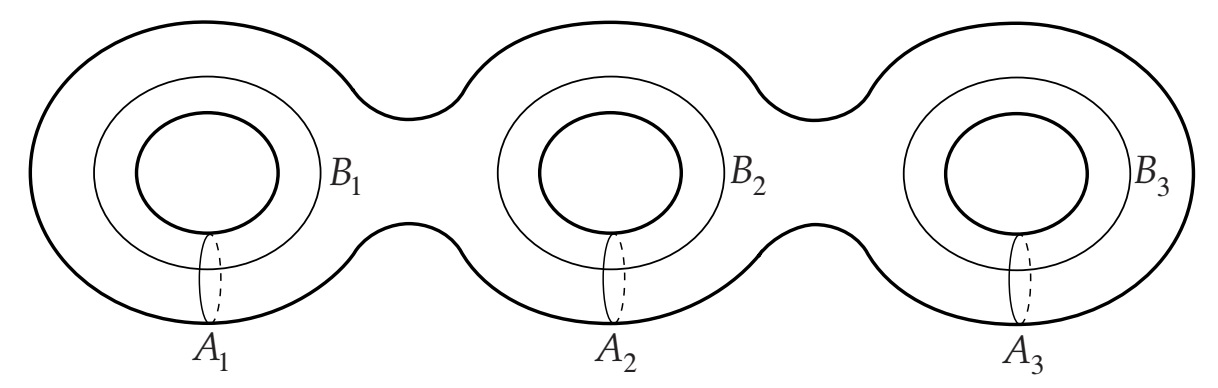
\includegraphics[width=0.8\textwidth]{figure/Fig9.1.jpg}\\
		\caption{A genus 3 surface, with $A$-cycles and $B$-cycles marked.}\label{Fig9.1}
	\end{center}
\end{figure}


The $A$-cycles and $B$-cycles are complete, in that every closed path is homotopic to a series of $A$-cycles or $B$-cycles.
In fact, they are overcomplete: the path
\begin{equation}
	(A_{1} B_{1}^{-1} A_{1}^{-1} B_{1})(A_{2} B_{2}^{-1} A_{2}^{-1} B_{2}) \ldots(A_{g} B_{g}^{-1} A_{g}^{-1} B_{g}) \label{9.2.4}
\end{equation}
can be contracted to a point, and the corresponding product must be the identity.
Counting moduli, there are 6 real parameters in each $PSL(2, \mathds{R})$ element, giving $6g$, subtracting 3 from the constraint \eqref{9.2.4}, 
and since the total $PSL(2, \mathds{R})$ gives an equivalent surface, subtract another 3, totaling $6g-6$.

Although the Schottky parametrization is similar to the Fuchsian parametrization, they have quite different properties. In particular, the complex structure of the latter is less obvious, and correspondingly, the extension to superstrings is not as simple.
\subsection*{Period Matrix}
The moduli parameter $\tau$ of the torus can be naturally generalized to a $g \times g$ matrix at genus $g$. To see this, we first need Abelian differentials or holomorphic 1-forms. 
They are world-sheet fields $\omega_{a}$ with the following properties in complex coordinates:
\begin{equation}
	\partial_{\bar{z}} \omega_{z} = 0 \:, \quad \omega_{\bar{z}} = 0 \:.
	\label{9.2.5}
\end{equation}
There are exactly $g$ such fields, and $g$ further satisfies conjugation relations. This originates from the Riemann-Roch theorem \eqref{5.3.22}. The Abelian differentials \eqref{9.2.5} and their conjugates are exactly the kernel of the operator $P_{0}^{T}$, 
for which the Riemann-Roch theorem is:
\begin{equation}
	\operatorname{dim} \operatorname{ker} P_{0}^{T}-\operatorname{dim} \operatorname{ker} P_{0}=-\chi=2 g-2 \:.
	\label{9.2.6}
\end{equation}
The operator $P_{0}$ acts on the scalar fields $c$ and $\tilde{c}$ with $h=0$, thus reducing to the ordinary gradient. There are always 2 zero modes ($c=$ constant or $\tilde{c}=$ constant), 
hence $\operatorname{dim}\operatorname{ker}P_{0}^{T}=2g$.
\begin{tcolorbox}[breakable]
	\begin{remark}
		Conventions. As in Chapter \ref{cha:5}, $P_n$ maps tensors with $n$ lower $z$ indices (and their conjugates) to $n+1$ indices, $P_n\colon t_{z\cdots z}\mapsto\nabla_{\bar z}t_{z\cdots z}$ up to normalization. Dimensions count independent solutions in the holomorphic and antiholomorphic sectors together. With this counting the Riemann--Roch theorem reads
		\begin{equation*}
			\dim\ker P_n-\dim\ker P_n^T=(2n+1)\chi ,
		\end{equation*}
		and for $n=1$ it is the familiar statement $\#\text{CKVs}-\#\text{moduli}=3\chi$. For $n=0$ the fields are the weight-zero ghosts $c,\tilde c$ of the text:
		\begin{align*}
			\ker P_0&=\{\partial_{\bar z}c=0,\ \partial_z\tilde c=0\}\eqs{1}\{c=\text{const},\ \tilde c=\text{const}\},\qquad\dim\ker P_0=2,\\
			\ker P_0^T&=\{\partial_{\bar z}\omega_z=0,\ \partial_z\omega_{\bar z}=0\},\qquad
			\dim\ker P_0^T\eqs{2}2-\chi=2g .
		\end{align*}
		At (1) a holomorphic function on a compact surface is constant. At (2) Riemann--Roch with $n=0$ was used. The kernel of $P_0^T$ consists of the holomorphic 1-forms $\omega_z\,\dif z$ and their complex conjugates, so there are exactly $g$ Abelian differentials. The same number follows from Hodge theory: the space of real harmonic 1-forms has dimension $b_1=2g$, and every harmonic form splits uniquely as $\omega+\bar\omega$ with $\omega$ holomorphic.
	\end{remark}
\end{tcolorbox}

Line integrals of 1-forms are coordinate invariants.
Then the natural basis for Abelian differentials is $\omega_{z i}, i=1, \ldots, g$, defined as:
\begin{equation}
	\oint_{A_{i}} \dif z \: \omega_{z j}=\delta_{i j} \:.
	\label{9.2.7}
\end{equation}
Then the period matrix:
\begin{equation}
	\tau_{i j}=\oint_{B_{i}} \dif z\: \omega_{z j} \label{9.2.8}
\end{equation}
characterizes the complex structure of the surface. When the genus is 1, $\omega_{z}$ is a constant, which is the usual $\tau$.

It can be proven that $\tau_{ij}$ is symmetric, so it has $\frac{1}{2} g(g+1)$ complex parameters.
When $g=1,2,3$ it equals the number of complex moduli. 
When $g \geq 4$, it will be larger, so not all period matrices correspond to Riemann surfaces.
The $\theta$-function \eqref{7.2.36} has a natural genus-$g$ generalization, 
where $\tau$ becomes the period matrix, and $\nu, n, a, b$ become $g$-component vectors.
\begin{tcolorbox}[breakable]
	\begin{proof}[Symmetry and positivity of $\tau_{ij}$]
		Cut $M$ along the cycles $A_k,B_k$ to obtain a simply connected $4g$-gon $F$ with boundary $\prod_kA_kB_kA_k^{-1}B_k^{-1}$, with the orientation for which the intersection number is $A_k\cdot B_l=\delta_{kl}$. For closed 1-forms $\alpha,\beta$, write $\alpha=\dif f$ on $F$. The values of $f$ on the two copies of an edge differ by a period of $\alpha$, which gives the Riemann bilinear relation
		\begin{equation*}
			\int_M\alpha\wedge\beta=\oint_{\partial F}f\beta=\sum_{k=1}^g\Bigl(\oint_{A_k}\alpha\oint_{B_k}\beta-\oint_{B_k}\alpha\oint_{A_k}\beta\Bigr).
		\end{equation*}
		With $\alpha=\omega_i=\omega_{zi}\dif z$ and $\beta=\omega_j$, the left side vanishes because $\dif z\wedge\dif z=0$:
		\begin{equation*}
			0\eqs{1}\sum_k\bigl(\delta_{ki}\tau_{kj}-\tau_{ki}\delta_{kj}\bigr)=\tau_{ij}-\tau_{ji} .
		\end{equation*}
		At (1) the normalization \eqref{9.2.7} and the definition \eqref{9.2.8} were used. So $\tau$ is symmetric. For positivity, take $\omega=\sum_ic_i\omega_i=f(z)\dif z$ with $c\in\mathbb C^g$ nonzero, and $\beta=\bar\omega$, whose periods are complex conjugated:
		\begin{align*}
			\int_M\omega\wedge\bar\omega&\eqs{2}\sum_k\bigl(c_k(\bar\tau\bar c)_k-(\tau c)_k\bar c_k\bigr)\eqs{3}-2\mi\,c^T(\operatorname{Im}\tau)\bar c ,\\
			\int_M\omega\wedge\bar\omega&=\int_M|f|^2\,\dif z\wedge\dif\bar z=-2\mi\int_M|f|^2\,\dif x\wedge\dif y .
		\end{align*}
		At (2) $\oint_{A_k}\omega=c_k$ and $\oint_{B_k}\omega=(\tau c)_k$. At (3) the symmetry of $\tau$ was used. Comparing the two lines, $c^T(\operatorname{Im}\tau)\bar c=\int|f|^2\,\dif x\,\dif y>0$, so $\operatorname{Im}\tau$ is positive definite. This is exactly what makes the genus-$g$ theta function $\sum_{n\in\mathbb Z^g}\exp(\pi\mi\,n\cdot\tau\cdot n+2\pi\mi\,n\cdot\nu)$ converge.

		Counting: a symmetric complex $g\times g$ matrix has $\frac12g(g+1)$ entries, compared with $3g-3$ complex moduli for $g\ge2$ (and 1 for $g=1$):
		\begin{equation*}
			g=1:\ 1=1,\qquad g=2:\ 3=3,\qquad g=3:\ 6=6,\qquad g=4:\ 10>9,
		\end{equation*}
		and for $g\ge4$ the difference $\frac12(g-2)(g-3)$ is positive. That is why only a subvariety of period matrices comes from Riemann surfaces.
	\end{proof}
\end{tcolorbox}

\subsection*{Hyperelliptic Surfaces}

There is another description that is sometimes very useful.
Consider the space $S_{2} \times S_{2}$ with coordinates $z$ and $y$. Consider the submanifold given by the following equation:
\begin{equation}
	y^{2}=\prod_{i=1}^{2 k}(z-Z_{i}) \:, \label{9.2.9}
\end{equation}
where $Z_{i}$ are complex parameters. Projected onto the $z$-coordinate, there are two surfaces connected by $k$ branch cuts.
This gives a surface with $g=k-1$ handles. When projected to $z$, the branch points are singular, 
but the entire surface \eqref{9.2.9} is not singular: $y$ is a good local coordinate.

This surface depends on $2k$ complex $Z_{i}$, but some are redundant under Möbius transformations, leaving $2k-3=2g-1$ complex parameters. When $g=1,2$, this is the same as the number of moduli;
but when $g \geq 3$, the number of moduli is larger, and only special surfaces take the form of \eqref{9.2.9}, which are called hyperelliptic surfaces.
\begin{tcolorbox}[breakable]
	\begin{remark}
		\emph{Genus.} The projection $(z,y)\mapsto z$ is a double cover of the sphere. It is branched at the $2k$ roots $Z_i$ and not at $z=\infty$, because the degree $2k$ is even: $y\approx\pm z^k$ gives two distinct points there. The Riemann--Hurwitz formula, $\chi(M)=2\chi(S_2)-\sum_{\text{branch points}}(e-1)$ with ramification index $e=2$, gives
		\begin{equation*}
			2-2g\eqs{1}2\cdot2-2k\cdot1=4-2k\quad\Longrightarrow\quad g=k-1 .
		\end{equation*}
		At (1) each branch point was counted with $e-1=1$. Near $Z_1$, $y^2\approx C(z-Z_1)$ with $C=\prod_{i\ne1}(Z_1-Z_i)\ne0$, so $z-Z_1\approx y^2/C$. Thus $y$ is a good coordinate at the branch point, while $z$ is two-to-one there.

		\emph{Parameters.} The $2k$ branch points modulo the 3 complex M\"obius parameters leave $2k-3=2(g+1)-3=2g-1$. Compared with $3g-3$ (or 1 at $g=1$): $g=1$ gives $1=1$, $g=2$ gives $3=3$, and $g=3$ gives $5<6$. The deficit $(3g-3)-(2g-1)=g-2$ grows with $g$.
	\end{remark}
\end{tcolorbox}

\section{Sewing and cutting world-sheets}  \label{sec:9.3}

A useful concept in analyzing string amplitudes is the relationship between higher genus amplitudes and lower genus amplitudes. The key element is the plumbing fixture. 
This is used to construct higher genus surfaces from lower genus ones.
Consider two world-sheets $M_{1}, M_{2}$ with coordinates $z_{1}, z_{2}$. 
We can connect them to form a new world-sheet $M$ as follows: Let $q$ be a complex parameter. Subtract a disk $|z_{1}|<(1-\epsilon)|q|^{1/2}$ from $M_{1}$, 
and subtract $|z_{2}|<(1-\epsilon)|q|^{1/2}$ from $M_{2}$, where $\epsilon$ is a small quantity.
To form a surface, identify points such that:
\begin{equation}
	z_{1} z_{2}=q \:. \label{9.3.1}
\end{equation}
As shown in Figure \ref{Fig9.2}. The disk regions:
\begin{equation}
	(1-\epsilon)^{-1}|q|^{1/2} > |z_{1}| > (1-\epsilon)|q|^{1/2} \label{9.3.2}
\end{equation}
are sewn together as shown in the figure. A representation of this construction is:
\begin{equation}
	M=M_{1} \infty M_{2}(z_{1}, z_{2}, q) \:. \label{9.3.3}
\end{equation}
This notation emphasizes that the corresponding surface depends on the choice of local coordinates.
If different local coordinates $z_{1}^{\prime}$ and $z_{2}^{\prime}$ are chosen, different circles will be cut out, and the connecting surfaces will generally be different. 
These two coordinate charts might also be located in different parts of a single surface $M_{0}$. Then the plumbing fixture construction adds a handle to the surface. This is denoted as:
\begin{equation}
	M=M_{0} 8(z_{1}, z_{2}, q)  \:. \label{9.3.4}
\end{equation}
The symbols `$\infty$' and `8' are used to distinguish the two sewing processes. The parameter $q$ is not strictly necessary—taking $z_{1}^{\prime}=z_{1} q^{-1/2}$, $z_{2}^{\prime}=z_{2} q^{-1/2}$, 
and $q^{\prime}=1$ gives an equivalent surface.
Introducing $q$ is to facilitate the discussion of the behavior as $q$ varies when the coordinate charts are fixed.

\begin{figure}[!htbp]
	\begin{center}
		%width=0.8\textwidth,bb=0 0 877 729
		%1px=0.75pt
		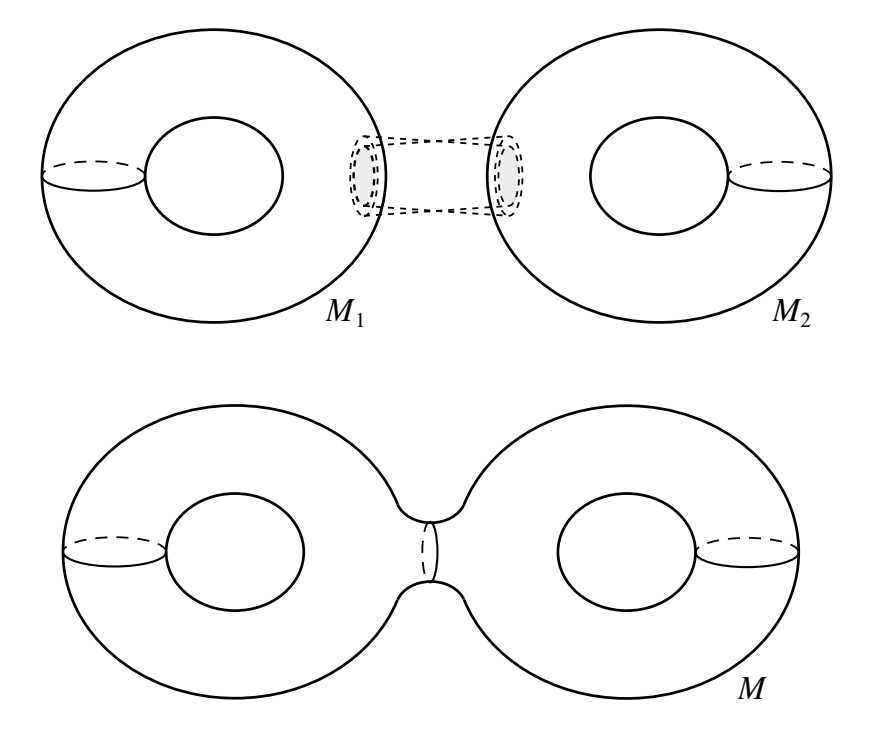
\includegraphics[width=0.8\textwidth]{figure/Fig9.2.jpg}\\
		\caption{Removing a disk from each of two world-sheets and then gluing the edges of the disks together.}\label{Fig9.2}
	\end{center}
\end{figure}

We can also reverse this construction. Given any Riemann surface $M$ and a non-intersecting curve $C$ on it, one can always find holomorphic coordinates $z_{1}=z_{2}^{-1}$ in a neighborhood of $C$ 
such that $C$ is given by $|z_{1}| = |z_{2}| = |q|^{1/2}$.
Cutting $C$ (undoing the equivalence relation $z_{1} z_{2}=q$) and gluing back disks $|z_{1}|<|q|^{1/2}$ and $|z_{2}|<|q|^{1/2}$ produces $M_{1}$ and $M_{2}$ (or $M_{0}$), 
such that $M$ can be regenerated through the sewing operation—depending on whether cutting $C$ makes the surface disconnected, we use sewing \eqref{9.3.3} or \eqref{9.3.4}, respectively.


\begin{figure}[!htbp]
	\begin{center}
		%width=0.8\textwidth,bb=0 0 994 578
		%1px=0.75pt
		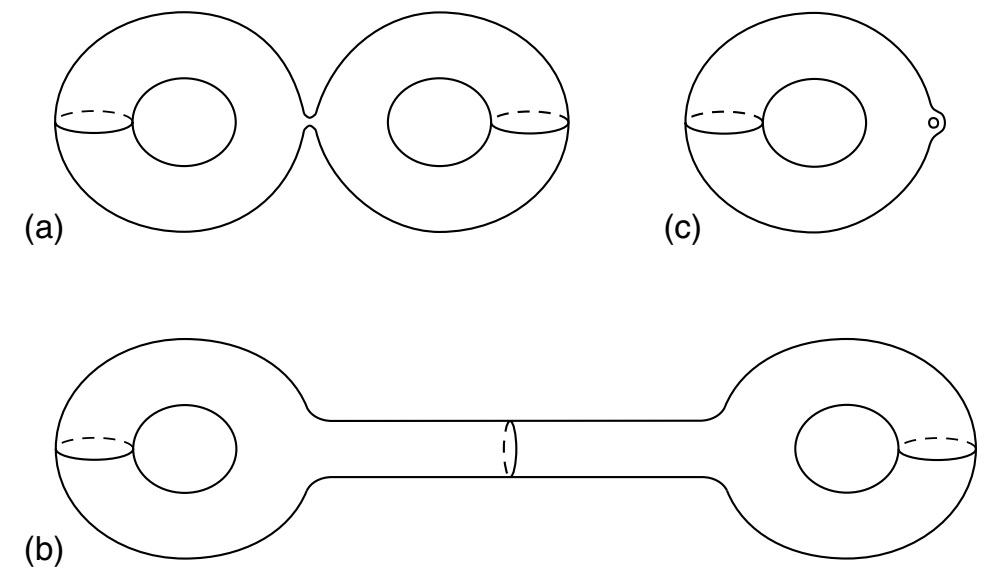
\includegraphics[width=0.8\textwidth]{figure/Fig9.3.jpg}\\
		\caption{Three representations of a genus 2 surface with degenerate circles.}\label{Fig9.3}
	\end{center}
\end{figure}

For the genus 2 example in Figure \ref{Fig9.2}, consider the case where $q \ll 1$.
Figure \ref{Fig9.3}a shows $M$ in this situation. 
In the overlapping region, we smoothly insert a metric between $\dif z_{1} \dif \bar{z}_{1}$ and $\dif z_{2} \dif \bar{z}_{2}$. 
The surface is pinched into a circle with a radius of order $|q|^{1/2} $. Through a Weyl transformation, one can always find a metric such that the radius remains of order 1, as shown in Figure \ref{Fig9.3}b.
Since the action of a Weyl transformation is isometric, its effect is that the handle's length becomes very large, of order $-\ln |q|$. The handle regions $|z_{1}|<1, |z_{2}|<1$ are equivalent to a cylinder:
\begin{equation}
	\ln |q|<\operatorname{Im} w<0 \:, \quad w \cong w+2 \pi \:.
	\label{9.3.5}
\end{equation}
where $z_{1}=\exp (-\mi w)$ and $z_{2}=q \exp (\mi w) $.
\begin{tcolorbox}[breakable]
	\begin{remark}
		The two coordinates are compatible with the sewing, since $z_1z_2=\me^{-\mi w}q\me^{\mi w}=q$. Writing $w=u+\mi v$,
		\begin{equation*}
			|z_1|=\me^{v}<1\iff v<0,\qquad |z_2|=|q|\me^{-v}<1\iff v>\ln|q| ,
		\end{equation*}
		and $w\cong w+2\pi$ because $z_1,z_2$ are single valued. The overlap of the two unit disks is therefore the cylinder \eqref{9.3.5}, with circumference $2\pi$ and length $-\ln|q|$. In the flat metric $\dif w\,\dif\bar w=\dif z_1\dif\bar z_1/|z_1|^2$, which is Weyl equivalent to $\dif z_1\dif\bar z_1$, the handle becomes a long tube as $q\to0$.
	\end{remark}
\end{tcolorbox}
\noindent Figure \ref{Fig9.3}c gives another representation of the same surface.
The disk regions $O(|q|)<|z|<O(1)$ around the small handles are conformally equivalent to the long cylinder in Figure \ref{Fig9.3}b. 
In the form of Figure \ref{Fig9.3}a, this picture can be considered as a Weyl transformation where all $M_{2}$ have been reduced.
In all these pictures, it is clear that the surface becomes special in the limit $q \rightarrow 0$. This handle is called a pinch or degenerate. This is an example of a boundary of moduli space. 
Moduli space boundaries are very important because every divergence must originate here. In fact, we will see that every boundary is in this form, where one or more handles are pinched. 
For a genus-2 surface, there is another way a single handle can degenerate if the $A$-cycle or $B$-cycle pinches.
This corresponds respectively to starting from a single torus and constructing a genus-2 torus via the `8' operation (rather than from two tori via the `$\infty$' operation) and taking $q \rightarrow 0$.

By repeatedly using the cutting operation, we will find an interesting fact: every Riemann surface will degenerate into spheres with 3 punctures. A puncture is a marked point with a specific complex coordinate near it; 
this is the data required for plumbing fixture sewing. In other words, every Riemann surface can be constructed from spheres with 3 punctures via sewing. For example, Figure \ref{Fig9.4} gives three ways to construct a genus 2 surface with 4 vertex operators. 
For each sewing operation, there is a complex modulus $q$. For each construction in Figure \ref{Fig9.4}, this gives 7 single complex moduli.
These correspond to the $3g-3=3$ complex moduli of a genus 2 surface plus the 4 positions of the vertex operators.

\begin{figure}[!htbp]
	\begin{center}
		%width=0.8\textwidth,bb=0 0 954 553
		%1px=0.75pt
		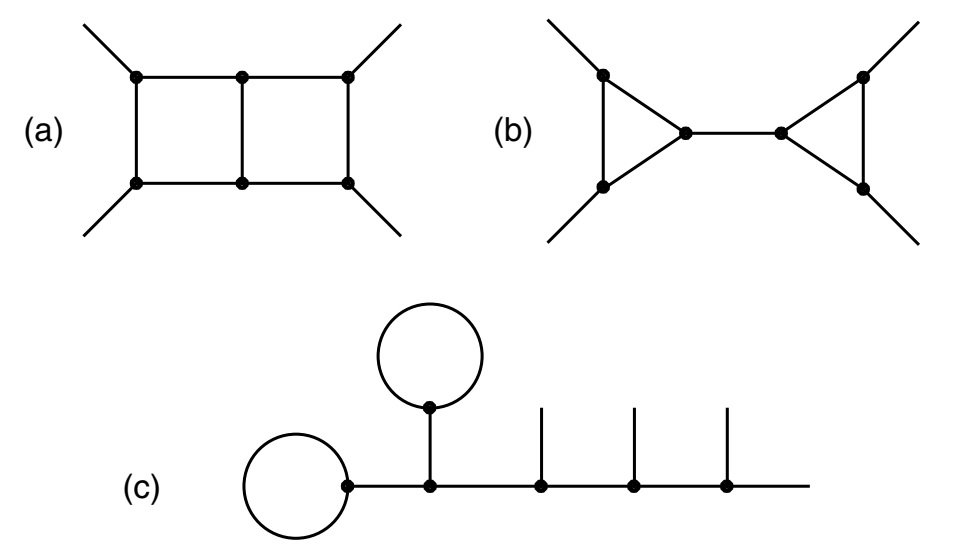
\includegraphics[width=0.8\textwidth]{figure/Fig9.4.jpg}
		\caption{Some sewing constructions for genus 2 surfaces with 4 operators. Each vertex is a sphere with three holes, each internal line represents a plumbing fixture construction, and each external line represents a vertex operator.}\label{Fig9.4}
	\end{center}
\end{figure}

\subsection*{Graph-theoretic decomposition}

Figure \ref{Fig9.4} is reminiscent of Feynman diagrams. We now describe a Feynman-like diagrammatic decomposition of the moduli space. The vertices are much more complicated than in \ref{Fig9.4}, potentially with any number of external lines and internal corrections in string loops. 
The key to this construction lies in making the properties of the moduli space boundary obvious.

The statement is: the integral over the moduli space is given by a sum over Feynman diagrams.
The internal propagator lines in the diagram represent the sewing operation, with the sewing parameter $q$ to be integrated out being in some standard region, such as $|q|<1$.  
The $n$-point vertices represent Riemann surfaces with $n$ punctures. We will see that surfaces in the vertices are to be integrated over some internal part of the moduli space and summed over genus. 
The sewing operation refers to specifying complex coordinates for each point to be sewn, so the vertex definition must include the choice made at each point. The set of surfaces of genus $g$ appearing in the $n$-point vertex is denoted as $\mathscr{V}_{g,n}$. 
External lines represent vertex operators.
\begin{figure}[!htbp]
	\begin{center}
		%width=0.8\textwidth,bb=0 0 343 313
		%1px=0.75pt
		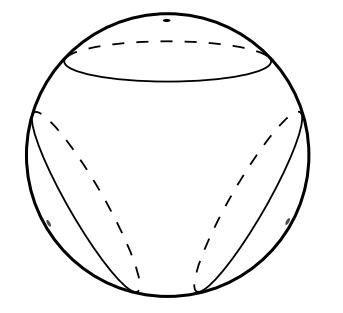
\includegraphics[width=0.8\textwidth]{figure/Fig9.5.jpg}\\
		\caption{A trilinear vertex, a sphere with three marked points and three sewing circles.}\label{Fig9.5}
	\end{center}
\end{figure}

We illustrate this construction with an example. Starting from the three-point vertex $\mathscr{V}_{0,3}$, as shown in Figure \ref{Fig9.5}, it is a sphere with 3 marked points and 3 sewing circles. 
In the complex coordinates near the corresponding points, the sewing circles are unit circles. Steps to build a sphere with four points: take two such vertices, remove the interior of one sewing circle from each, and then glue them at both ends of a cylinder; 
this is equivalent to the plumbing fixture construction. This corresponds to the Feynman diagram in Figure \ref{Fig9.6}a; the cylinder length is $-\ln |q|$ (with circumference adjusted to $2\pi$).
Integrating over $|q|<1$ 
and summing over the other two channels only gives a part of the integration region of the sphere with four points, as shown in Figure \ref{Fig9.6}b. The shaded region is covered, but the non-shaded region is missing.

\begin{figure}[!htbp]
	\begin{center}
		%width=0.8\textwidth,bb=0 0 987 482
		%1px=0.75pt
		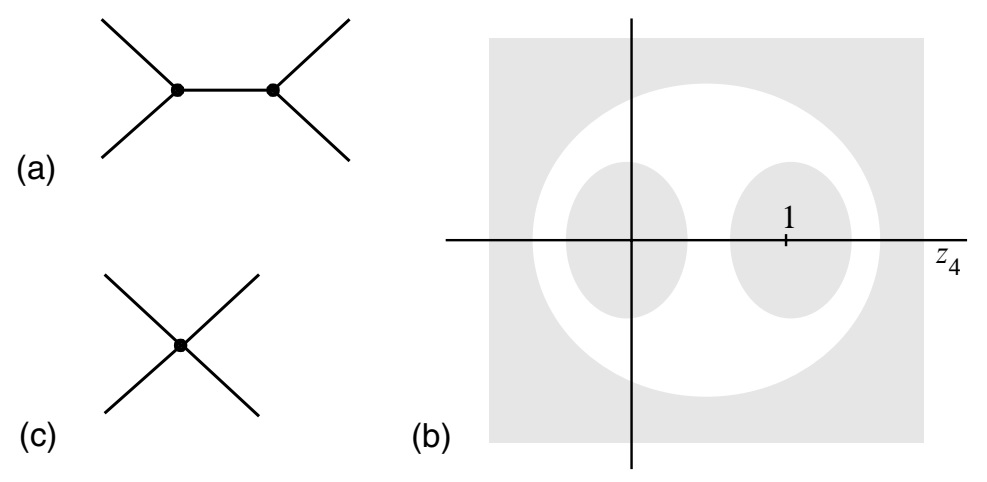
\includegraphics[width=0.8\textwidth]{figure/Fig9.6.jpg}\\
		\caption{(a) Constructing a sphere with four vertex operators. (b) The region covered by this diagram in the $z$-plane. (c) Additional vertex required to give the correct amplitude. Integration for a four-hole sphere in the non-shaded region.}\label{Fig9.6}
	\end{center}
\end{figure}

Let us provide further explanation.
For trilinear vertices, place the points at $0,1, \infty$ on the sphere, and choose coordinate systems $z^{(0)}, z^{(1)}$, $z^{(\infty)}$, 
so the three sewing circles are $|z^{(0,1, \infty)}|=1$. This choice should be invariant under the 6 Möbius transformations that permute the vertices, making the vertex symmetric.
There are multiple possible choices, for example:
\begin{equation}
	z^{(0)}=\frac{a z}{z-2}, \quad z^{(1)}=\frac{a(z-1)}{z+1}, \quad z^{(\infty)}=\frac{a}{2 z-1} \:, \label{9.3.6}
\end{equation}
where $a$ is an arbitrary constant. When $a \geq 3$, the sewing circles do not overlap, ensuring that the plumbing fixture construction gives a good surface for all $q \leq 1$.
Readers can prove that sewing the $z^{(\infty)}$ and $z^{(0)}$ coordinate charts from two spheres under parameter $q$ produces a sphere with vertex operators at $0,1, \frac{1}{2}(1+a^{2}/q)$ and $\frac{1}{2}(1-a^{2}/q)$. 
Under Möbius transformation, this is equivalent to vertex operators at $0,1, \infty$, and:
\begin{equation}
	z_{4}=(q-a^{2})^{2}/4 a^{2} q \:.
	\label{9.3.7}
\end{equation}
\begin{tcolorbox}[breakable]
	\begin{remark}
		\emph{The sewing circles.} The disk $|z^{(0)}|<1$ is $|z|<|z-2|/a$, an Apollonius disk for the points $0,2$ with ratio $1/a$. Its center is $-2/(a^2-1)$ and its radius $2a/(a^2-1)$, so on the real axis it spans $[-2/(a-1),\,2/(a+1)]$. The map $z\to1-z$ sends $z^{(0)}\to z^{(1)}$, so the disk around $1$ spans $[(a-1)/(a+1),\,(a+1)/(a-1)]$. The disk around $\infty$ is $|z^{(\infty)}|<1$, i.e.\ $|z-\frac12|>\frac a2$. Hence
		\begin{align*}
			\text{disks at }0,1\text{ disjoint}&\iff\frac{2}{a+1}\le\frac{a-1}{a+1}\iff a\ge3,\\
			\text{disk at }0\text{ inside }|z-\tfrac12|\le\tfrac a2&\iff\frac12+\frac{2}{a-1}\le\frac a2\iff(a-1)^2\ge4\iff a\ge3 .
		\end{align*}
		At $a=3$ the three circles touch pairwise, at $z=\frac12$ and $z=-1,2$. For $a>3$ they are disjoint, so the plumbing fixture is well defined for all $|q|\le1$.

		\emph{The sewn sphere.} Sew sphere $A$ with its $z^{(\infty)}$ chart to sphere $B$ (coordinate $z'$) with its $z'^{(0)}$ chart, $z^{(\infty)}z'^{(0)}=q$. The map is M\"obius, so it extends to a global identification of $B$ with $A$:
		\begin{equation*}
			\frac{a}{2z-1}=\frac{q(z'-2)}{az'}\quad\Longrightarrow\quad z=\frac12\Bigl(1+\frac{a^2}{q}\frac{z'}{z'-2}\Bigr).
		\end{equation*}
		The surviving operators of $B$ are at $z'=1$ and $z'=\infty$, where $z'/(z'-2)=-1$ and $1$. They land at $z_\mp=\frac12(1\mp a^2/q)$, while the operators of $A$ stay at $0$ and $1$. This proves the statement in the text. Now send $z_+\to\infty$ with the M\"obius map $f(z)=z(1-z_+)/(z-z_+)$, which fixes $0$ and $1$:
		\begin{equation*}
			z_4=f(z_-)=\frac{z_-(1-z_+)}{z_--z_+}\eqs{1}\frac{\frac{q-a^2}{2q}\cdot\frac{q-a^2}{2q}}{-a^2/q}=-\frac{(q-a^2)^2}{4a^2q} .
		\end{equation*}
		At (1) $z_-=1-z_+=(q-a^2)/2q$ and $z_--z_+=-a^2/q$. The other assignment, $z_-\to\infty$, gives $(q+a^2)^2/4a^2q=1-f(z_-)$ instead. All six cross-ratio values follow from $\lambda=f(z_-)$ by $\lambda\to1-\lambda$ and $\lambda\to1/\lambda$. For generic $q$ none of them equals the expression printed in \eqref{9.3.7}, which is $-f(z_-)$. With the charts \eqref{9.3.6} and $z_1z_2=q$, the correct value is therefore $z_4=-(q-a^2)^2/4a^2q$ or one of its cross-ratio images; the printed sign appears to be a typo. The statement that matters is unaffected: $|z_4|\approx a^2/4|q|\to\infty$ as $q\to0$, and $|q|\le1$ maps to a neighborhood of $z_4=\infty$ (for $|q|=1$, $|z_4|\ge(a^2-1)^2/4a^2$). This neighborhood is the outer shaded region of Figure \ref{Fig9.6}b.
	\end{remark}
\end{tcolorbox}
As $q$ runs over the unit disk, $z_{4}$ covers the outer shaded region of Figure \ref{Fig9.6}b. Permuting the vertices gives the other two regions. 
We could try to take smaller $a$, so that the shaded regions grow, but they will eventually overlap and double-count some surfaces, while other surfaces still will not be produced. 
They will never exactly cover the entire plane, so we also need to add an explicit four-point vertex $\mathscr{V}_{0,4}$, given by a sphere with 4 marked points, 
and integrate over the non-shaded region of the $z$-plane.
Since there is still a choice for each hole's coordinate for each value of $z_{4}$, this does not completely define $\mathscr{V}_{0,4}$. 
Connect the boundaries of the shaded and non-shaded regions in a smooth way. Note that the Feynman diagram in Figure \ref{Fig9.6}a contains all asymptotic regions $z_{4} \rightarrow 0,1, \infty$, 
while the four-point vertex only contains non-degenerate surfaces. Then the behavior in this limit is clearly given by the limit $q \rightarrow 0$: this is why plumbing fixture construction is useful.

As an example, sewing two circles of a single vertex at both ends of a cylinder gives a torus with one vertex operator.
This covers the $\operatorname{Im} \tau \rightarrow \infty$ limit of the torus moduli space, but the internal region is lost and must be added back through a manual vertex region $\mathscr{V}_{1,1}$.

This construction can be extended inductively. Each sewing operation always adds:
\begin{equation}
	r = 3g + n - 2  \label{9.3.8}
\end{equation}
parameters.
The original sphere with three holes, vertex $\mathscr{V}_{0,3}$, has $r=1$. The `8' operation gives $r=r_{0}+1$, while the `$\infty$' operation gives $r=r_{1}+r_{2}$. 
Thus, $\mathscr{V}_{0,4}$ and $\mathscr{V}_{1,1}$ both have $r=2$. It has been proven that $\mathscr{V}_{g, n}$ can be constructed by induction on $r$, 
thus covering the entire moduli space as claimed earlier.
\begin{tcolorbox}[breakable]
	\begin{remark}
		Note $r=(3g-3+n)+1=\dim_{\mathbb C}\mathscr M_{g,n}+1$, one more than the number of complex moduli of a genus-$g$ surface with $n$ punctures. The rules quoted follow directly:
		\begin{align*}
			\mathscr V_{0,3}:&\quad r=0+3-2=1,\\
			\text{`8'}:\ (g,n)\to(g+1,n-2):&\quad r'=3(g+1)+(n-2)-2=r+1,\\
			\text{`}\infty\text{'}:\ (g_1,n_1),(g_2,n_2)\to(g_1+g_2,n_1+n_2-2):&\quad r'=3(g_1+g_2)+n_1+n_2-4=r_1+r_2 .
		\end{align*}
		Each sewing introduces one complex parameter $q$, which matches the moduli count. Under `8', $3g-3+n$ increases by $3-2=1$. Under `$\infty$', $\dim\mathscr M_{g_1+g_2,n_1+n_2-2}=\dim\mathscr M_{g_1,n_1}+\dim\mathscr M_{g_2,n_2}+1$. For example, $\mathscr V_{0,4}$ and $\mathscr V_{1,1}$ both have $r=2$, one modulus. For Figure \ref{Fig9.4}, a graph with only cubic vertices, $V$ vertices, $E$ internal lines and $n$ external lines satisfies $3V=2E+n$ and $E-V+1=g$. Hence $E=3g-3+n$: for $g=2$, $n=4$ this gives $7$ plumbing parameters, the $3+4$ complex moduli quoted in the text.
	\end{remark}
\end{tcolorbox}
A clearer construction is given below. On any Riemann surface, there exists a unique minimum-area metric, defined as the metric with minimum area subject to the constraint that every non-trivial closed curve has a length of at least $2\pi$. 
Each point on this surface lies on at least one saturating geodesic, a non-trivial closed curve with length exactly $2\pi$. 
Saturating geodesics that can be continuously transformed into other saturating geodesics do not intersect themselves, and each set of homotopic saturating geodesics forms an annulus (topologically a torus) on the surface. 
Different annuli cover the entire surface but may overlap. The height $h$ of such an annulus is defined as the shortest distance between its two boundary geodesics. The idea of a minimum-area metric can be extended to surfaces with holes 
by treating circles around the holes as non-trivial.
The minimum-area metric near a hole is of the form $\dif z \dif \bar{z} / z \bar{z}$, a semi-infinite cylinder of radius $2\pi$. 
Thus there are two types of annuli: one internal and finite, the other gathering at holes and semi-infinite, terminating inside the surface.

We can now use this construction to describe $\mathscr{V}_{g, n}$.
Take all Riemann surfaces with $n$ holes, imposing the constraint that any internal annulus has a height less than $2\pi$ under the minimum-area metric. 
Cut the semi-infinite cylinders, leaving a stub of length $\pi$, and glue them into usual disks, inserting vertex operators at the bottom of the stubs. With these vertices, the sum of Feynman diagrams will exactly cover the moduli space once. 
It can be proven that sewing minimum-area surfaces still produces minimum-area surfaces.
Annuli with height less than $2\pi$ are clearly contained in the vertices, while annuli with height greater than $2\pi$ will be produced by the sewing operators on the stubs, 
with the corresponding height being $2\pi$ from the stubs plus $-\ln |q|$ from the plumbing fixture; as $q$ is integrated, this runs from $2\pi$ to $\infty$. The minimum length constraint and maximum height ensure that degenerate surfaces do not appear in the vertices, 
so they only appear when one or more $q$ tend to zero, which is exactly what was to be proven.
\section{Sewing and cutting CFTs} \label{sec:9.4}



\begin{figure}[!htbp]
	\begin{center}
		%width=0.8\textwidth,bb=0 0 957 668
		%1px=0.75pt
		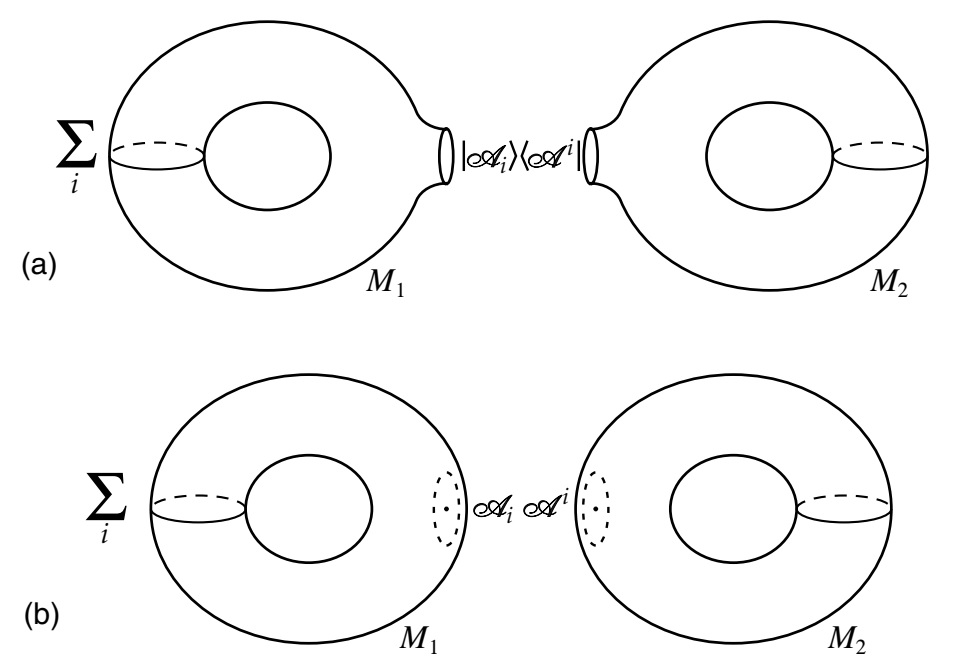
\includegraphics[width=0.8\textwidth]{figure/Fig9.7.jpg}\\
		\caption{(a) Cutting the path integral on $M$ by inserting a complete set of boundary states. (b) Each state is replaced by a disk with a local operator.}\label{Fig9.7}
	\end{center}
\end{figure}

By sewing lower genus Riemann surfaces together, we described higher genus Riemann surfaces. Using the sewing properties of the path integral, similarly, CFTs on higher genus surfaces can be associated with lower-order amplitudes. This relationship is shown in Figure \ref{Fig9.7}.
For clarity, we first discuss the case $q=1$. The path integral on $M$ is cut along the circle $|z_{1}|=|z_{2}|=1$, inserting a complete set of boundary states. Then each boundary state is replaced by a disk with a corresponding local operator, 
leaving the uncut world-sheets $M_{1}$ and $M_{2}$.
The precise form of this result is:
\begin{equation}
	\langle {}_{\cdots 1} {}_{\cdots 2}\rangle_{M} = \sum_{i j}\Bigl \langle {}_{\cdots 1} \mathscr{A}_{i}^{(z_{1})}\Bigr\rangle_{M_{1}} 
	\mathsf{G}^{ij} \Bigl\langle\mathscr{A}_{j}^{(z_{2})} {}_{\cdots 2}\Bigr\rangle_{M_{2}} \:.
	\label{9.4.1}
\end{equation}
We allow arbitrary additional insertions ${}_{\cdots 1}$ and ${}_{\cdots 2}$ on $M_{1}$ and $M_{2}$; they must be located outside the circles $|z_{1}|=1$ and $|z_{2}|=1$. 
We have not yet specified any particular orthogonality for this basis; an appropriate invertible matrix $\mathsf{G}^{i j}$ still needs to be decided.
Instead of the handles, the insertions $\mathscr{A}_{i}$ and $\mathscr{A}_{j}$ 
are implicitly located at the origins of the $z_{1}$ and $z_{2}$ coordinate systems, respectively.

Now consider the case where $M_{2}$ is a sphere, let the sewing coordinate $z_{2}$ be denoted as $u$, and let ${}_{\cdots 2}$ be a local operator $\mathscr{A}_{k}$ at $z=0$.
From the plumbing fixture construction, we have $z_{1} u=1$, and from the sphere, we have $z u=1$, so we can extend $z_{1}=z$ to the entire sewing region. 
The sewn surface $M$ is the same as $M_{1}$ with an extra operator $\mathscr{A}_{k}$ at $z_{1}=0$.
Then \eqref{9.4.1} becomes:
\begin{equation}
	\Bigl \langle {}_{\cdots 1} \mathscr{A}_{k}^{(z_{1})}\Bigr\rangle_{M_{1}} = 
	\sum_{i j}\Bigl\langle {}_{\cdots 1} \mathscr{A}_{i}^{(z_{1})}\Bigr\rangle_{M_{1}} \mathsf{G}^{ij} 
	\Bigl\langle\mathscr{A}_{j}^{(u)} \mathscr{A}_{k}^{(z)}\Bigr\rangle_{S_{2}} \:.
	\label{9.4.2}
\end{equation}
The two-point function $\langle\mathscr{A}_{j}^{(u)} \mathscr{A}_{k}^{(z)}\rangle_{S_{2}}$ is exactly the inner product $\lAngle j \vert k\rangle=\mathsf{G}_{jk}$. 
Then \eqref{9.4.2} implies:
\begin{equation}
	\mathsf{G}^{ij} \mathscr{G}_{jk} = \delta_{k}^{i} \label{9.4.3}
\end{equation}
or:
\begin{equation}
	\mathsf{G}^{ij} = \mathscr{G}^{ij} \:. \label{9.4.4}
\end{equation}
That is, the inner product defined by the two-point function on the sphere is exactly what is needed for sewing.
Thus, for $M_{2}$ being a sphere containing an arbitrary local operator, we have derived \eqref{9.4.1}. 
Through state-operator isomorphism, any boundary state can be obtained in this way. Since the path integral is trivial, this result only depends on the sewing region but is independent of the rest of the surface, 
so it holds for any $M_{2}$ and ${}_{\cdots 2}$.
Sewing with parameter $q$ is equivalent to sewing with $q=1$ and local coordinates $z_{1}$ and $z_{2}^{\prime}=z_{2} / q$. 
Thus, we obtain \eqref{9.4.1} for $\mathscr{A}_{j}$ in the primed coordinate system, thereby obtaining an extra factor from the conformal transformation back to $z_{2}$:
\begin{equation}
	\mathscr{A}_{j}^{(z_{2}^{\prime})}=q^{h_{j}} \bar{q}^{\tilde{h}_{j}} \mathscr{A}_{j}^{(z_{2})} \:.
	\label{9.4.5}
\end{equation}
The result is:
\begin{equation}
	\langle {}_{\cdots 1 \cdots 2} \rangle_{M} = \sum_{ij} q^{h_{j}} \tilde{q}^{\tilde{h}_{j}} 
	\Bigl\langle {}_{\cdots 1} \mathscr{A}_{i}^{(z_{1})}\Bigr\rangle_{M_{1}} \mathscr{G}^{i j} 
	\Bigl\langle\mathscr{A}_{j}^{(z_{2})} {}_{\cdots 2} \Bigr\rangle_{M_{2}} \:, \label{9.4.6}
\end{equation}
where we have taken a basis diagonal with respect to the weights.
\begin{tcolorbox}[breakable]
	\begin{remark}
		The identification $z_1z_2=q$ is the same as $z_1z_2'=1$ with $z_2'=z_2/q$, so \eqref{9.4.1} (the $q=1$ sewing) applies with $\mathscr A_j$ defined in the $z_2'$ frame. The change of frame $z_2=qz_2'$ is a pure dilation, generated by $L_0,\tilde L_0$ alone, so an operator of weights $(h_j,\tilde h_j)$ transforms without mixing even if it is not primary:
		\begin{equation*}
			\mathscr A_j^{(z_2')}(0)\eqs{1}\Bigl(\frac{\partial z_2}{\partial z_2'}\Bigr)^{h_j}\Bigl(\frac{\partial\bar z_2}{\partial\bar z_2'}\Bigr)^{\tilde h_j}\mathscr A_j^{(z_2)}(0)=q^{h_j}\bar q^{\tilde h_j}\mathscr A_j^{(z_2)}(0).
		\end{equation*}
		At (1) the transformation law for a dilation was used; the higher terms of \eqref{2.9.6} involve $L_{n>0}$ and are absent because $\partial^2z_2/\partial z_2'^2=0$. Substituting into \eqref{9.4.1} gives \eqref{9.4.6}, with $\bar q^{\tilde h_j}$. The same substitution in the `8' version gives \eqref{9.4.7}. For $q\to0$ the sum is dominated by the lowest weights, $q^{h_j}\bar q^{\tilde h_j}$ with the smallest $h_j+\tilde h_j$ first, exactly as in an OPE.
	\end{remark}
\end{tcolorbox}
For the `8' operation, the path integrals on $M$ and $M_{0}$ are related in the same way:
\begin{equation}
	\langle {}_{\cdots}\rangle_{M}=\sum_{i j} q^{h_{j}} \bar{q}^{\tilde{h}_{j}} \mathscr{G}^{ij} 
	\Bigl\langle {}_{\cdots 1} \mathscr{A}_{i}^{(z_{1})} \mathscr{A}_{j}^{(z_{2})}\Bigr\rangle_{M_{0}} \:. \label{9.4.7}
\end{equation}

Consider again the boundary of moduli space, given by $q \rightarrow 0$ for one or more handles. We see that low-weight operators will control this behavior.
\eqref{9.4.6} and \eqref{9.4.7} are similar to the OPE; in fact, when $M_{2}$ is a sphere and ${}_{\cdots 2}$ is a pair of vertex operators, \eqref{9.4.6} reduces to the OPE. 
This analogy is obvious from Figure \ref{Fig9.3}c, which represents this limit as the insertion of a small handle. The sewing relation shows that not just operator products, but a small handle, or any perturbation we can sew into a small circle, 
are equivalent to a sum of local operators. \eqref{9.4.6} is a beautiful generalization of the OPE.
From the perspective of $M_{1}$, a tiny $M_{2}$ is glued near $z_{1}=0$. 
This can be expanded with local operators $\mathscr{A}_{i}$, and the coefficient function is $\langle\mathscr{A}^{i} {}_{\cdots 2}\rangle_{M_{2}}$.
From the perspective of $M_{2}$, a tiny $M_{1}$ is glued near $z_{2}=0$, and it can be expanded with $\mathscr{A}^{i}$, 
and the coefficient function is $\langle {}_{\cdots 1} \mathscr{A}_{i}\rangle_{M_{1}}$.

We have argued that every Riemann surface can degenerate to a sphere with 3 holes. Therefore, the sewing construction relates all amplitudes to the three-point amplitudes on the sphere, which are clearly operator product coefficients: they are the data defining the CFT. 
We will encounter many equivalences between CFTs—we have already seen T-duality, and bosonization will be another noteworthy example.
The sewing construction provides a criterion for whether two theories are equal: 
a one-to-one mapping between their states and identity OPEs.\footnote{We should note that if multiple (2,0) plus (0,2) fields can act as $T_{ab}$, as in the free field example in Section \ref{sec:2.5}, it must be specified which is the energy-momentum tensor. This choice determines the conformal transformation of the operators, which implicitly enters the sewing operation.} In fact, we will prove in Chapter 15 that the operator products of the primary fields alone determine the operator products of all other fields. 

Let's explore this idea further. We can cut a surface along various different curves, so to guarantee the sewing relation, the expectation value on $M$ always gives the same result. 
First consider infinitesimal transformations on the cutting curve $C$.
Generally, infinitesimal transformations that leave $M$ invariant can be obtained by making infinitesimal transformations to the coordinates used for sewing:
\begin{subequations} \label{9.4.8}
	\begin{align}
		z_{1}^{\prime} &= z_{1} + \sum_{n=-\infty}^{\infty} \epsilon_{n} z_{1}^{n+1}  \:, \label{9.4.8a} \\
		z_{2}^{\prime} &= z_{2} - \sum_{n=-\infty}^{\infty} \epsilon_{-n} q^{-n} z_{2}^{n+1} \:.
		\label{9.4.8b}
	\end{align}
\end{subequations}
Then the difference in the sewing expression is proportional to:
\begin{align}
	\mathscr{A}_{i}^{(z_{1}^{\prime})} \mathscr{G}^{ij} \mathscr{A}_{j}^{(z_{2}^{\prime})} - 
	\mathscr{A}_{i}^{(z_{1})} \mathscr{G}^{ij} \mathscr{A}_{j}^{(z_{2})} 
	&= -\sum_{n=-\infty}^{\infty} \epsilon_{n} \Bigl[L_{n} \cdot \mathscr{A}_{i}^{(z_{1})} \mathscr{G}^{ij} \mathscr{A}_{j}^{(z_{2})} \nonumber \\
	&\quad -\mathscr{A}_{i}^{(z_{1})} \mathscr{G}^{ij} L_{-n} \cdot \mathscr{A}_{j}^{(z_{2})}\Bigr]+\text{(anti-holomorphic)} \:, \label{9.4.9}
\end{align}
where we have used the conformal transformation \eqref{2.9.6}, and the anti-holomorphic part represents taking $\epsilon_{n} \rightarrow \epsilon_{n}^{*}$ and $L_{n} \rightarrow \tilde{L}_{n}$.
The discussion used to derive \eqref{9.4.4} can be used to prove that the quantity in the braces is zero. This is equivalent to saying that we can pull the contour integral defining the generator through the sewing handle; 
the change from $L_{n}$ to $L_{-n}$ comes from the reversal of coordinates. All other conserved charge contour integrals can also be pulled over.
\begin{tcolorbox}[breakable]
	\begin{remark}
		\emph{Derivation of \eqref{9.4.8b}.} The surface is unchanged if the identification $z_1z_2=q$ still holds in the new coordinates, i.e.\ $z_2'=q/z_1'$. To first order,
		\begin{equation*}
			z_2'=\frac{q}{z_1\bigl(1+\sum_n\epsilon_nz_1^n\bigr)}\eqs{1}z_2\Bigl(1-\sum_n\epsilon_nz_1^n\Bigr)\eqs{2}z_2-\sum_n\epsilon_nq^nz_2^{1-n}\eqs{3}z_2-\sum_n\epsilon_{-n}q^{-n}z_2^{n+1} .
		\end{equation*}
		At (1) the expansion was taken to first order in $\epsilon$. At (2) $z_1=q/z_2$. At (3) $n\to-n$.

		\emph{Derivation of \eqref{9.4.9}.} By \eqref{2.9.6}, under $z'=z+\sum_n\varepsilon_nz^{n+1}$ an operator at the origin changes as $\mathscr A^{(z')}=\mathscr A^{(z)}-\sum_n\varepsilon_nL_n\cdot\mathscr A^{(z)}$ plus the antiholomorphic part. For $z_1$, $\varepsilon_n=\epsilon_n$. For $z_2$, $\varepsilon_n=-\epsilon_{-n}q^{-n}$, so
		\begin{equation*}
			\mathscr A_j^{(z_2')}=\mathscr A_j^{(z_2)}+\sum_n\epsilon_{-n}q^{-n}L_n\cdot\mathscr A_j^{(z_2)}=\mathscr A_j^{(z_2)}+\sum_n\epsilon_nq^{n}L_{-n}\cdot\mathscr A_j^{(z_2)} .
		\end{equation*}
		Multiplying out to first order and setting $q=1$ gives \eqref{9.4.9}. For general $q$ the factor $q^n$ combines with $q^{h_j}$ into $q^{h_j+n}$, the weight of $L_{-n}\cdot\mathscr A_j$.

		\emph{The bracket vanishes.} Write $L_n\cdot\mathscr A_i=\sum_k(\ell_n)_{ki}\mathscr A_k$, and let $\mathsf G$ be the matrix $\mathscr G_{ij}=\lAngle i|j\rangle$. Then
		\begin{align*}
			\sum_{ij}(L_n\cdot\mathscr A_i)\mathscr G^{ij}\mathscr A_j=\sum_{kj}(\ell_n\mathsf G^{-1})_{kj}\mathscr A_k\mathscr A_j,\qquad
			\sum_{ij}\mathscr A_i\mathscr G^{ij}(L_{-n}\cdot\mathscr A_j)=\sum_{il}(\mathsf G^{-1}\ell_{-n}^T)_{il}\mathscr A_i\mathscr A_l ,
		\end{align*}
		so the two agree if $\mathsf G\ell_n=\ell_{-n}^T\mathsf G$, that is, $\lAngle k|L_n|i\rangle=\lAngle L_{-n}k|i\rangle$. This is the BPZ conjugation law for the map $u=1/z$ used in the sewing. With $T(z)=u^4T'(u)$ and $\dif z=-\dif u/u^2$,
		\begin{equation*}
			L_n=\oint_0\frac{\dif z}{2\pi\mi}z^{n+1}T(z)\eqs{4}\oint_0\frac{\dif u}{2\pi\mi}u^{-n+1}T'(u)=L'_{-n},
		\end{equation*}
		where at (4) the minus sign from $\dif z$ cancels against the reversal of orientation of the contour. So pulling the Virasoro generators through the sewing handle turns $L_n$ into $L_{-n}$, and the bracket in \eqref{9.4.9} vanishes.
	\end{remark}
\end{tcolorbox}

There are also sets of curves that cannot be related by continuous transformations. By cutting circles around different pairs of operators, the four-point amplitude on the sphere can be written in the form of three-point amplitudes. The equivalence between different sewings is the result of the OPE associativity, 
see Figure \ref{Fig2.8}.

Another example is given by the torus: by cutting along the $A$-cycle or $B$-cycle, or any other non-self-intersecting closed curve, we can make the torus degenerate to a sphere.
In terms of a plane with an equivalence relation, a closed curve $C$ starting at $(\sigma^{1}, \sigma^{2})=(0,0)$ must end at an equivalent point:
\begin{equation}
	2 \pi(m, n) \:. \label{9.4.10}
\end{equation}
All curves with the same $m$ and $n$ values can be continuously transformed into each other, so we need to examine what the relationship is between sewing curves with different $m$ and $n$.
It can be proven that for non-trivial non-self-intersecting curves, $m$ and $n$ must be coprime, which implies that there exist integers $p$ and $q$ such that $m p-n q=1$.
Then there exists another modular transformation:
\begin{equation}
	(\sigma^{1}, \sigma^{2}) = (\sigma^{\prime 1}, \sigma^{\prime 2}) \begin{bmatrix}
		m & n \\
		q & p		
	\end{bmatrix} \:, \label{9.4.11}
\end{equation}
such that the curve $C$ returns to:
\begin{equation}
	(\sigma^{\prime 1}, \sigma^{\prime 2})=2 \pi(1,0) \:, \label{9.4.12}
\end{equation}
\begin{tcolorbox}[breakable]
	\begin{remark}
		Input (a standard fact about the torus): a non-trivial simple closed curve is homotopic to a straight line from $0$ to $2\pi(m,n)$ with $\gcd(m,n)=1$. If $\gcd=d>1$, the straight line closes already at $2\pi(m,n)/d$ and runs $d$ times around a primitive loop, and no curve in that class is simple. Given coprime $m,n$, B\'ezout's identity gives integers $p,q$ with $mp-nq=1$. Then
		\begin{equation*}
			M=\begin{bmatrix}m&n\\q&p\end{bmatrix},\qquad\det M=mp-nq=1,\qquad
			2\pi(1,0)\,M=2\pi(m,n) .
		\end{equation*}
		So $M\in SL(2,\mathbb Z)$, and in the primed coordinates the curve $C$ runs from $0$ to $2\pi(1,0)$, which is the $A$-cycle. Since $M$ and $M^{-1}$ are integer matrices, the identifications $\sigma\cong\sigma+2\pi\mathbb Z^2$ and $\sigma'\cong\sigma'+2\pi\mathbb Z^2$ are the same. The primed coordinates describe the same torus, with $\tau$ replaced by its image under the corresponding modular transformation.
	\end{remark}
\end{tcolorbox}
which is the $A$-cycle.
So cutting along a non-trivial non-self-intersecting curve is equivalent to cutting along the $A$-cycle on a modular equivalent value of $\tau$. Thus, the compatibility of the sewing construction is equivalent to modular invariance.

Through two successive operations, each set of sewing curves can be transformed into each other: the four-point associativity transformation on the sphere, and the modular transformation on the torus containing one vertex operator. Figure \ref{Fig9.4} makes this quite believable. 
For example, Figure \ref{Fig9.4}a is related to Figure \ref{Fig9.4}b through an associativity condition. Repeated use of associativity can bring the sewing to the form of Figure \ref{Fig9.4}c, where all loops are represented as one-loop one-point functions. 
So, they are the conditions for defining a reasonable set of operator product coefficients for any conformal field theory. This program for solving dual constraints is called the conformal bootstrap.
This is only possible with the introduction of additional constraints. We will discuss this in Chapter 15.

The considerations of this section can be extended to world-sheets with boundaries, where there will be degenerate bands in addition to degenerate handles. Compatibility conditions have been generalized to this situation.

\section{General amplitudes}  \label{sec:9.5}
We have now gathered all the elements needed to understand the compatibility of general string amplitudes. 

Given the graphical decomposition of the moduli space, the sewing theory allows us to give a graphical representation of general string amplitudes. First consider the propagator from the plumbing fixture construction.
The ghost insertion for modulus $q$ is:
\begin{equation}
	\oint \frac{\dif z}{2 \pi \mi} \: b_{z_{1} z_{1}} \frac{\partial z_{1}}{\partial q}\biggr|_{z_{2}}=\frac{b_{0}}{q} \:, \label{9.5.1}
\end{equation}
similarly, for $\bar{q}$ it is $\tilde{b}_{0} / \bar{q}$.
Introducing these insertions and using the sewing expression \eqref{9.4.6}, the factor attached to the propagator is:
\begin{equation}
	\int_{|q|<1} \frac{\dif^{2} q}{q \bar{q}} \: q^{\alpha^{\prime}(k_{i}^{2}+m_{i}^{2})/4} 
	\bar{q}^{\alpha^{\prime}(k_{i}^{2}+\tilde{m}_{i}^{2})/4} \mathscr{G}^{ij} b_{0} \tilde{b}_{0}
	= \frac{8 \pi \delta_{m_{i}^{2}, \tilde{m}_{i}^{2}} \mathscr{G}^{ij} b_{0} \tilde{b}_{0}}{\alpha^{\prime}(k_{i}^{2}+m_{i}^{2}-\mi \epsilon)} \:.
	\label{9.5.2}
\end{equation}
\begin{tcolorbox}[breakable]
	\begin{remark}
		\emph{Ghost insertion \eqref{9.5.1}.} From $z_1=q/z_2$ at fixed $z_2$, $\partial z_1/\partial q=1/z_2=z_1/q$, so
		\begin{equation*}
			\oint\frac{\dif z_1}{2\pi\mi}b_{z_1z_1}\frac{\partial z_1}{\partial q}\Bigr|_{z_2}=\frac1q\oint\frac{\dif z_1}{2\pi\mi}z_1b(z_1)=\frac{b_0}{q},
		\end{equation*}
		exactly as in the remark after \eqref{9.1.34}.

		\emph{Propagator \eqref{9.5.2}.} The sewing formula \eqref{9.4.6} supplies $q^{h_i}\bar q^{\tilde h_i}$ for each intermediate state, with $h_i=L_0=\frac{\alpha'}{4}(k_i^2+m_i^2)$ and $\tilde h_i=\frac{\alpha'}{4}(k_i^2+\tilde m_i^2)$. The measure $\dif^2q$ comes with $b_0\tilde b_0/q\bar q$. Hence
		\begin{equation*}
			\int_{|q|<1}\frac{\dif^2q}{q\bar q}q^{h_i}\bar q^{\tilde h_i}=\int_{|q|<1}\dif^2q\,q^{h_i-1}\bar q^{\tilde h_i-1}\eqs{1}\frac{8\pi}{\alpha'}\frac{\delta_{m_i^2,\tilde m_i^2}}{k_i^2+m_i^2-\mi\epsilon} .
		\end{equation*}
		At (1) this is literally the integral \eqref{9.1.22}, with the same analytic continuation. The number of real moduli is $m=6g-6+2n$: $6g-6$ for the surface and 2 for each puncture.
	\end{remark}
\end{tcolorbox}
By inserting vertex operators on the surfaces appearing in the vertices of the sewing construction, the $n$-string coupling is given as:
\begin{equation}
	g(i_{1}, \ldots, i_{n}) = \sum_{g} \int_{\mathscr{V}_{g, n}} \dif^{m} t  \:
	\biggl\langle\prod_{k=1}^{m} B_{k} \prod_{l=1}^{n} \hat{\nu}_{i_{l}}\biggr\rangle_{g} \:.
	\label{9.5.3}
\end{equation}
where $m=6 g+2 n-6$ is the number of moduli. Then Feynman diagrams constructed from the coupling \eqref{9.5.3} and propagator \eqref{9.5.2} regenerate the entire string amplitude. 
The index $i$ still represents the state and momentum of each string. The tree-level amplitude in Section \ref{sec:9.1} illustrates this result.

The first issue is the finiteness of amplitudes. We assert that divergences can only come from the boundary of the space. Just like what happened in various low-order amplitudes. At finite values of the moduli, the sewing formula gives a sum over infinite string states, 
but since this sum is essentially an expansion of a quantum state in a complete basis, the sum is convergent. In fact, convergence can only be guaranteed in a unitary CFT, 
but the non-unitary part of the string CFT is quite tame.
The $X^{0}$ CFT is defined by analytic continuation from a unitary CFT, while the ghost CFT simply generates the Faddeev-Popov determinant, so it is finite. 
Now the boundary as the $q \rightarrow 0$ limit of various propagators becomes obvious, and the integral \eqref{9.5.2} has been encountered several times before. It is defined through analytic continuation and gives the ordinary field theory propagator. 
Thus the only singularity is the pole in the propagator, which represents the generation of on-shell particles in the intermediate state. In particular, they are long-range rather than short-range divergences. 

Another issue is unitarity, which we explored in some detail for four-point tree-level amplitudes.
Bringing the general amplitude into Feynman diagram form, rather than solving the combinatorics in detail, 
we can cite the results from standard field theory regarding the unitarity of graphical representations. Furthermore, it was illustrated at the end of Section \ref{sec:9.1} that the sum over intermediate states will reduce to a sum over physical states, 
a result that will generalize as in field theory. 

In conclusion, the issues involved in perturbative finiteness and unitarity in string theory are easily understood. Note again that we have not assumed 26 flat dimensions, but only $d$ flat dimensions plus a compact positive-norm CFT with central charge $26-d$. 
Of course, for bosonic strings, since flat spacetime is not its solution, any discussion of the unitarity of the flat spacetime S-matrix is somewhat formalistic—first, there is the problem of tachyon stability. Second, there is the cosmological constant problem introduced by loops.

Another method for proving the finiteness and unitarity of string theory is based on the light-cone gauge. This method has also been greatly developed.
This gauge gives up covariance, but it has significant advantages—it makes it possible to give an explicit description of the moduli space, 
and amplitudes can be expressed in field theory form, with the Hamiltonian local with respect to light-cone time $x^{+}$. By proving that perturbation theory is equivalent to covariant perturbation theory, covariance is established.

\subsection*{String divergence}


\begin{figure}[!htbp]
	\begin{center}
		%width=0.8\textwidth,bb=0 0 937 514
		%1px=0.75pt
		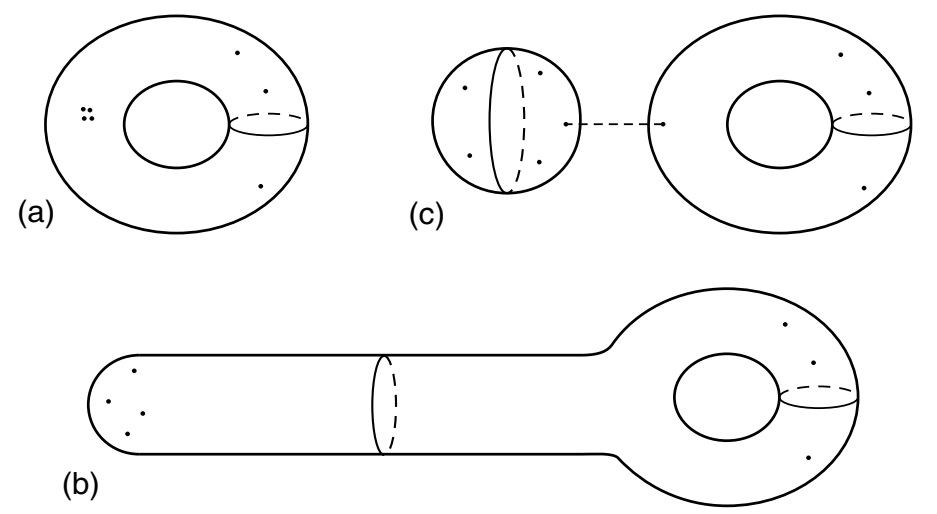
\includegraphics[width=0.8\textwidth]{figure/Fig9.8.jpg}\\
		\caption{(a) A torus with $n$ vertex operators, where $m$ are clustered together. (b) Conformally equivalent image: these $m$ vertex operators are at the end of a long cylinder. 
			(c) Sewing construction, represented as the product of a sphere with $m{+}1$ vertex operators and a torus with $n{-}m{+}1$ vertex operators.}\label{Fig9.8}
	\end{center}
\end{figure}

Before moving forward, we provide further explanation that string divergences are long-range.
Consider a one-loop amplitude with $n$ vertex operators, keeping $\tau$ fixed, and taking the limit where $m$ operators cluster together, as shown in Figure \ref{Fig9.8}. 
String loops certainly contain gravity, and when interactions cluster in spacetime, this has UV divergence. There is indeed a divergence in this string amplitude, but it comes from long-range spacetime distances, not short-range. 
Figure \ref{Fig9.8}b gives a conformally equivalent description, where $m$ vertex operators are connected to the remaining torus through a long cylinder.
Cutting the cylinder and inserting a complete set of states, 
we obtain the usual representation \eqref{9.5.2}, where $q \rightarrow 0$ becomes the limit of vertex operator clustering. So the only singularity is the pole of the propagator at long-range spacetime. 
Conformal invariance once again transforms short-range on the world-sheet into long-range in spacetime.

The cases $m=n$ and $m=n{-}1$ present special problems. When $m=n$, this means all vertex operators cluster together, and momentum conservation makes $k^{\mu}$ zero.
For massless states, the pole is $1/0$, 
and since momentum conservation forces the amplitude to stay on the pole, analytic continuation does not help. This is a tadpole diagram, as in Section \ref{sec:7.4}, and the solution is the same: corrections to the background field. 
The divergence here is proportional to the torus amplitude with one vertex operator.

Another problematic case is $m=n-1$, where all vertex operators cluster together except for one vertex operator $\mathscr{V}_{n}$. 
Momentum conservation requires the momentum flowing through the cylinder to be $k^{\mu}=-k_{n}^{\mu}$.
However, conformal invariance requires $k_{n}^{2}=-m_{n}^{2}$, so for those intermediate states with $m_{j}^{2}=m_{n}^{2}$, 
the momentum of the intermediate state is fixed at the top of a pole, as shown in Figure \ref{Fig9.9}: the intermediate propagator is $1/0$. As long as the internal line $j$ is the same as the external line $n$, divergence occurs. 
The explanation is quite simple. This loop represents a radiative correction to the mass of particle $n$. Define the S-matrix's external momentum as being on the true mass shell, which includes radiative corrections, and this still does not have this IR divergence.
Note that the problem here is not the UV divergence within the loop, but the IR divergence of the starred propagator, which happens even if the mass correction is finite. 
The solution in the string case is the same. The momentum appearing in the vertex operators must be at the true physical mass; in general, they are not the same as the tree-level mass, 
which are integer multiples of $1 / \alpha^{\prime}$. Note that for certain massless fields—especially gauge bosons—gauge invariance requires them to be massless to all orders.
Incidentally, for massive states, the mass shift is usually complex; these states are unstable and will decay to light string states.

\begin{figure}[!htbp]
	\begin{center}
		%width=0.8\textwidth,bb=0 0 435 233
		%1px=0.75pt
		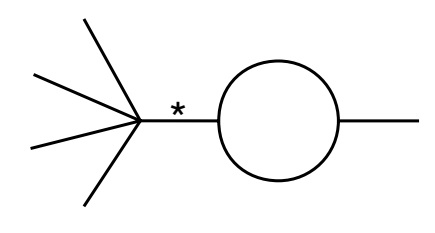
\includegraphics[width=0.8\textwidth]{figure/Fig9.9.jpg}\\
		\caption{Field theory diagram corresponding to the case $m=n{-}1$. Kinematics forces the starred propagator to diverge. The solution is the (finite) mass shift due to the loop.}\label{Fig9.9}
	\end{center}
\end{figure}


There is a question here. Earlier, when we studied the compatibility of string theory, world-sheet conformal invariance required the $\beta$-function \eqref{3.7.14} to be zero. 
These $\beta$-functions do not include information about high genus surfaces—they correspond to tree-level string field equations. What happens when we try to expand around the loop-corrected background? 
In fact, all problems are solved. The dangerous limits in Figure \ref{Fig9.8} give not only divergence but also conformal anomalies.
To see this, 
draw this limit as in \ref{Fig9.3}c, with a small handle glued onto the sphere. This small handle can be represented by a series of local operators; in particular, from the massless level there is:
\begin{equation}
	\partial X^{\mu} \bar{\partial} X_{\mu} \frac{\dif q \dif \bar{q}}{q \bar{q}} \:. \label{9.5.4}
\end{equation}
Now by requiring the size of the handle to be greater than $a$; that is, $|q|
\me^{\omega}>a$, where the metric on the sphere is $\dif z \dif \bar{z} \me^{2 \omega}$,  
the divergence is cut off in a coordinate-invariant way. The lower bound of the integral \eqref{9.5.4} gives:
\begin{equation}
	-4 \pi \partial X^{\mu} \bar{\partial} X_{\mu} \ln (a \me^{-\omega}) \:.
	\label{9.5.5}
\end{equation}
\begin{tcolorbox}[breakable]
	\begin{remark}
		With $q=r\me^{\mi\theta}$ and $\dif^2q=2r\,\dif r\,\dif\theta$, the handle integral runs over $a\me^{-\omega}<|q|<1$:
		\begin{equation*}
			\int_{a\me^{-\omega}<|q|<1}\frac{\dif^2q}{q\bar q}\eqs{1}2\int_0^{2\pi}\dif\theta\int_{a\me^{-\omega}}^1\frac{\dif r}{r}\eqs{2}-4\pi\ln\bigl(a\me^{-\omega}\bigr)=-4\pi\ln a+4\pi\omega .
		\end{equation*}
		At (1) $q\bar q=r^2$. At (2) the angular integral gives $2\pi$ and the radial one $-\ln(a\me^{-\omega})$. Multiplying by $\partial X^\mu\bar\partial X_\mu$ gives \eqref{9.5.5}. The dependence on the cutoff is logarithmic, and the piece $4\pi\omega\,\partial X\cdot\bar\partial X$ is an explicit dependence on the Weyl factor. It has the form of a shift of the metric coupling $\eta_{\mu\nu}\partial X^\mu\bar\partial X^\nu$, so it contributes a term proportional to $\eta_{\mu\nu}$ to $\beta^G_{\mu\nu}$.
	\end{remark}
\end{tcolorbox}
Thus, the Weyl factor of our metric has a new dependence: this corrects the Weyl anomaly $\beta_{\mu v}^{G}$ of the $\sigma$-model, \eqref{3.7.14}. 
To obtain a Weyl-invariant theory, the background must satisfy the full string loop-corrected Weyl invariance condition (or equivalently, BRST invariance). 
The Weyl anomaly from the offset background cancels the anomaly from the small handle, which is the Fischler-Susskind mechanism. From Figure \ref{Fig9.3}c, we can consider divergence and Weyl anomaly as world-sheet UV effects, 
which do not come from the usual short-wave fluctuations of fields, but from very small topological fluctuations. We should emphasize that for any fixed Riemann surface of any genus, the local structure is not affected by topology; 
what generates divergence and Weyl anomaly is the integration over Riemann surfaces.
This can also be considered as the failure of the cancellation of propagator discussion. Kinematics forces the amplitude to stay on the pole, and we cannot use analytic continuation to eliminate possible surface terms under BRST variation. 
In fact, their appearance corresponds to the Weyl anomaly \eqref{9.5.5}. In the loop-corrected background, the BRST anomaly from the background offset cancels the BRST anomaly generated by the moduli space boundary—assembling the string characteristics together gives a consistent spacetime picture.

Implementing this in string perturbation theory is quite cumbersome, but fortunately, it is rarely necessary. First, in most supersymmetric theories, the background is not corrected. 
Second, in string theory, it is most efficient to analyze long-range physics in two steps: first use string theory to derive the form of the low-energy effective action, and then use this theory for long-range. 
Then, we do not need to deal with IR divergence at the string theory level.
In the current case, the tadpole diagram gives the following potential energy term:
\begin{equation}
	\delta \bm{S}=-\sum_{\chi} \Lambda_{\chi} \int \dif^{d} x \: (-G)^{1/2} \me^{-\chi \Phi} \:. \label{9.5.6}
\end{equation}
Here $\Lambda_{\gamma}$ comes from the Euler number, and the dependence of the action on $\Phi$ comes from the fact that $\me^{\Phi}$ is the string coupling. 
After some effort, we can extract individual tadpole diagrams of gravitons and dilatons from string amplitudes.
The same concept extends to vertex operator corrections from mass shifts, and other IR divergences, for example, exclusive amplitudes in theories with massless particles. Since string theory degenerates into field theory at long-range, 
these field theory divergences must also appear in the corresponding string amplitudes. We emphasize again that UV divergences in field theory generally indicate basic limits to the theory's applicability, while IR divergences usually mean the wrong question was asked. 
Any such divergence is treated in string theory in the same way as in field theory.

Let's review what we have learned. For the specific moduli problem of bosonic strings, the S-matrix is finite and unitary. The basic mechanism is modular invariance, which cuts off UV divergence without breaking spacetime gauge invariance. 
Of course, knowing that string theory is reasonable in weak coupling perturbation theory around flat spacetime is far from enough.
We hope to know whether this theory is still reasonable beyond perturbation theory, and to have some means of calculating non-perturbative corrections. 
Additionally, we hope to know what string theory implies for the short-range properties of spacetime. In the rest of this chapter, we will briefly describe attempts in these directions.

\section{String field theory} \label{sec:9.6}

It is very interesting to compare the methods we use in string theory with those for constructing quantum field theories. World-sheet path integrals are similar to summing over particle paths, which is usually called the first quantization scheme. On the other hand, in quantum field theory, we can develop quantum field theory in the first quantization form, where interaction vertices must be introduced, i.e., where several particles cluster.
In string theory, the second step is unnecessary—there are no special points, and the sum over topologies generates the interactions. 
However, this result is just a perturbation expansion, and some phenomena will not appear in this expansion. In the Standard Model, this includes quark confinement and finite-temperature baryon number violation in weak interactions. 
There seems to be no way to make them appear in the resummed perturbation expansion; instead, they require a more general construction of the theory.

In the previous section, we expressed string amplitudes in the form of propagators and vertices, much like the perturbation theory of infinite-component field theories. 
Can we derive this form from an integration over an infinite set of spacetime fields? Are there some principles, extending gauge invariance and general coordinate invariance, that determine the form of the theory? 
This is the subject of string field theory.
We start from the following assumption: take the string wavefunction $\Psi[X]$ and promote it to a field operator, or equivalently a path integral variable—this is the so-called second quantization. 
Now, $\Psi[X]$ depends on the curve $X^{\mu}(\sigma)$ described by the string in spacetime. Roughly speaking, a string is created or annihilated in this configuration. 
However, we need to be more precise: should we require $\Psi$ to be invariant under reparametrization of the curve? And does it also depend on the Polyakov metric $g_{ab}$?
If we start from the BRST form of the theory, introduce Faddeev-Popov ghosts, and then second-quantize, everything seems fine. 
From the commutation relations, $b$ and $c$ are conjugate to each other, so if we consider $c$ and $\tilde{c}$ as coordinates, and the wavefunction is $\Psi[X, c, \tilde{c}]$, 
then we have a path integral over all these functionals:
\begin{equation}
	\int[\dif \Psi] \: \exp (\mi S[\Psi]) \:.
	\label{9.6.1}
\end{equation}
We first examine open strings and describe a specific approach. 

What symmetry will constrain the string action? From our study of string vertex operators and null states, we might guess it is the symmetry:
\begin{equation}
	\delta \Psi=Q_{\mathrm{B}} \Lambda \label{9.6.2}
\end{equation}
where $\Lambda$ is an arbitrary functional. The simplest action with this invariance is:
\begin{equation}
	S_{0}=\frac{1}{2}\lAngle\Psi |Q_{\mathrm{B}}| \Psi\rangle \:. \label{9.6.3}
\end{equation}
The equations of motion are:
\begin{equation}
	Q_{\mathrm{B}} \Psi=0 \:. \label{9.6.4}
\end{equation}
\begin{tcolorbox}[breakable]
	\begin{remark}
		Conventions. $\lAngle A|B\rangle$ is the BPZ inner product on the disk, which is nonzero only for total ghost number $3$. $Q_{\mathrm B}$ is BPZ-odd up to a sign, $\lAngle Q_{\mathrm B}A|B\rangle=\pm\lAngle A|Q_{\mathrm B}B\rangle$ (contour deformation on the sphere), and the pairing is symmetric on the ghost-number-1 fields used here. The field $\Psi$ has ghost number 1, like $c\mathscr V$, and $\Lambda$ has ghost number 0. The action \eqref{9.6.3} has total ghost number $1+1+1=3$. Varying,
		\begin{align*}
			\delta S_0&=\frac12\Bigl(\lAngle\delta\Psi|Q_{\mathrm B}|\Psi\rangle+\lAngle\Psi|Q_{\mathrm B}|\delta\Psi\rangle\Bigr)\eqs{1}\lAngle\delta\Psi|Q_{\mathrm B}|\Psi\rangle ,\\
			\delta_\Lambda S_0&=\lAngle Q_{\mathrm B}\Lambda|Q_{\mathrm B}|\Psi\rangle\eqs{2}\pm\lAngle\Lambda|Q_{\mathrm B}^2|\Psi\rangle=0 .
		\end{align*}
		At (1) the symmetry of the quadratic form was used. At (2) $Q_{\mathrm B}$ was moved across and $Q_{\mathrm B}^2=0$. The first line holds for arbitrary $\delta\Psi$, and the BPZ pairing is nondegenerate, so the equation of motion is $Q_{\mathrm B}\Psi=0$. That is the physical-state condition, and the gauge freedom $\Psi\to\Psi+Q_{\mathrm B}\Lambda$ is the BRST-null equivalence. Solutions modulo gauge are therefore the BRST cohomology at ghost number 1.
	\end{remark}
\end{tcolorbox}

One way to see its rationality is to expand the string field $\Psi$ into infinitely many ordinary fields, each corresponding to an internal state of the string.
Let $\Psi_{i}[X^{\prime}, c, \tilde{c}]$ be a complete basis of wavefunction for all internal modes except the center of mass $x^{\mu}$. Then a general state can be expressed as:
\begin{equation}
	\Psi[X, c, \tilde{c}]=\sum_{i} \Phi_{i}(x) \Psi_{i}[X^{\prime}, c, \tilde{c}] \:, \label{9.6.5}
\end{equation}
where the expansion coefficients are functions of the remaining variables $x^{\mu}$.
The path integral of the string field becomes an infinite product of the path integrals of the component functions:
\begin{equation}
	\int[\dif \Psi] \rightarrow \prod_{i} \int[\dif \Phi_{i}] \:. \label{9.6.6}
\end{equation}
As usual, we can start from the ground state functional $\Psi_{0}$ and use raising operators to build the remaining states.
For example, keeping only the states of the first two levels:
\begin{align}
	\Psi &= \Bigl[\varphi(x) + A_{\mu}(x) \alpha_{-1}^{\mu} + B(x) b_{-1} + C(x) c_{-1} + \varphi^{\prime}(x) c_{0}\nonumber \\
	&\qquad+A_{\mu}^{\prime}(x) \alpha_{-1}^{\mu} c_{0} + B^{\prime}(x) b_{-1} c_{0} + C^{\prime}(x) c_{-1} c_{0} + \cdots\Bigr] 
	\Psi_{0} \:.
	\label{9.6.7}
\end{align}
Here $\varphi$ is the tachyon field, $A_{\mu}$ is the gauge field, and $B$ and $C$ are the Faddeev-Popov ghost fields corresponding to spacetime gauge symmetry. 
The primed fields can always be gauged away, or they are auxiliary fields (i.e., they satisfy algebraic equations rather than differential equations and can be eliminated). 
The symmetry \eqref{9.6.2} can be verified to include the ordinary gauge transformation on $A_{\mu}$, while the action for $\varphi$ is in the Klein-Gordon form and for $A_{\mu}$ is in the Maxwell form. 
Thus BRST string field theory gives a very compact extension of spacetime gauge invariance.
\begin{tcolorbox}[breakable]
	\begin{remark}
		Conventions (Polchinski Ch.~4). Open string, $\Psi_0=|{\downarrow};k\rangle=c_1|0;k\rangle$ with $|0\rangle$ the $SL(2)$ vacuum, $\alpha_0^\mu=(2\alpha')^{1/2}k^\mu$, and $L_0^{\mathrm m}=\alpha'k^2+N$. The BRST charge is $Q_{\mathrm B}=\sum_nc_nL^{\mathrm m}_{-n}+(\text{ghost terms})$, and it annihilates $|0;0\rangle$. The BPZ map (open string, $u=-1/z$) sends a weight-$h$ mode $\phi_n\to(-1)^{n+h}\phi_{-n}$; the normalization $\mathcal K\equiv\langle0|c_{-1}c_0c_1|0\rangle$ is left as a convention. Keep the ghost-number-1 part of \eqref{9.6.7} at levels $0$ and $1$. Since $b_{-1}c_0\Psi_0=-c_0b_{-1}c_1|0\rangle=-c_0|0\rangle$, write $\beta\equiv-B'$:
		\begin{equation*}
			\Psi=\bigl[\varphi\,c_1+A_\mu\,\alpha^\mu_{-1}c_1+\beta\,c_0\bigr]|0;k\rangle ,\qquad \Lambda=\lambda\,b_{-1}\Psi_0=\lambda|0;k\rangle .
		\end{equation*}
		\emph{Gauge transformation.} Only the matter Virasoro modes feel the momentum, and only $c_0,c_1$ survive on $|0\rangle$:
		\begin{equation*}
			Q_{\mathrm B}\Lambda\eqs{1}\lambda\bigl(c_0L_0^{\mathrm m}+c_1L_{-1}^{\mathrm m}\bigr)|0;k\rangle\eqs{2}\lambda\bigl[\alpha'k^2\,c_0+(2\alpha')^{1/2}k\cdot\alpha_{-1}\,c_1\bigr]|0;k\rangle ,
		\end{equation*}
		so $\delta A_\mu=(2\alpha')^{1/2}k_\mu\lambda$ and $\delta\beta=\alpha'k^2\lambda$. At (1) the $k=0$ terms reproduce $Q_{\mathrm B}|0;0\rangle=0$, $c_{n\ge2}|0\rangle=0$, and $L^{\mathrm m}_{n\ge1}|0;k\rangle=0$. At (2) $L^{\mathrm m}_{-1}|0;k\rangle=\alpha_{-1}\cdot\alpha_0|0;k\rangle$. With $k\to-\mi\partial$ this is $\delta A_\mu\propto\partial_\mu\lambda$, the Maxwell gauge transformation.

		\emph{Action on each component.} The ghost pieces follow from $\{Q_{\mathrm B},c_p\}=\sum_{m+n=p}(1-n)c_mc_n$ (the mode form of $\delta c=c\partial c$) and $[Q_{\mathrm B},\alpha^\mu_{-1}]=\sum_nc_n\alpha^\mu_{-1-n}$. On $|0\rangle$ they give $\{Q_{\mathrm B},c_1\}|0\rangle=-c_0c_1|0\rangle$ and $\{Q_{\mathrm B},c_0\}|0\rangle=-2c_{-1}c_1|0\rangle$. Therefore
		\begin{align*}
			Q_{\mathrm B}\,c_1|0;k\rangle&\eqs{3}\bigl(\alpha'k^2-1\bigr)c_0c_1|0;k\rangle,\\
			Q_{\mathrm B}\,\alpha^\mu_{-1}c_1|0;k\rangle&\eqs{4}\alpha'k^2\,\alpha^\mu_{-1}c_0c_1|0;k\rangle+(2\alpha')^{1/2}k^\mu\,c_{-1}c_1|0;k\rangle,\\
			Q_{\mathrm B}\,c_0|0;k\rangle&\eqs{5}-2\,c_{-1}c_1|0;k\rangle-(2\alpha')^{1/2}k\cdot\alpha_{-1}\,c_0c_1|0;k\rangle .
		\end{align*}
		At (3) $Q_{\mathrm B}c_1=\{Q_{\mathrm B},c_1\}-c_1Q_{\mathrm B}$ and the result for $Q_{\mathrm B}|0;k\rangle$ were used. At (4) $[Q_{\mathrm B},\alpha_{-1}]$ contributes $c_0\alpha_{-1}+c_{-1}\alpha_0$, and the $-1$ of (3) cancels the $+1$ from $N=1$. At (5) $Q_{\mathrm B}c_0=\{Q_{\mathrm B},c_0\}-c_0Q_{\mathrm B}$ was used. So
		\begin{equation*}
			Q_{\mathrm B}\Psi=\varphi(\alpha'k^2-1)c_0c_1|0\rangle+\bigl[\alpha'k^2A_\mu-(2\alpha')^{1/2}k_\mu\beta\bigr]\alpha^\mu_{-1}c_0c_1|0\rangle+\bigl[(2\alpha')^{1/2}k\cdot A-2\beta\bigr]c_{-1}c_1|0\rangle ,
		\end{equation*}
		which is invariant under the gauge transformation above: $\alpha'k^2(2\alpha')^{1/2}k\lambda-(2\alpha')^{1/2}k\,\alpha'k^2\lambda=0$ and $2\alpha'k^2\lambda-2\alpha'k^2\lambda=0$.

		\emph{Action.} The BPZ bras are $\langle0;-k|c_{-1}$, $\langle0;-k|\alpha^\nu_1c_{-1}$, and $-\langle0;-k|c_0$. Their only nonzero pairings are
		\begin{equation*}
			\langle0|c_{-1}\,c_0c_1|0\rangle=\mathcal K,\qquad\langle0|\alpha_1^\nu c_{-1}\,\alpha^\mu_{-1}c_0c_1|0\rangle=\eta^{\mu\nu}\mathcal K,\qquad-\langle0|c_0\,c_{-1}c_1|0\rangle=\mathcal K ,
		\end{equation*}
		so all three components are weighted by the same $\mathcal K$. The string-field reality condition makes $\varphi,A_\mu$ real and $\beta=\mi B$ with $B$ real. That is what makes the cross term real in position space, where $k\cdot A(-k)\beta(k)\to\mi B\,\partial\cdot A$ up to sign. Then, with $k\to-\mi\partial$,
		\begin{align*}
			S_0&=\frac{\mathcal K}{2}\int\dif^dx\Bigl[\alpha'\partial\varphi\cdot\partial\varphi-\varphi^2+\alpha'\partial_\nu A_\mu\partial^\nu A^\mu+2(2\alpha')^{1/2}B\,\partial\cdot A+2B^2\Bigr]\\
			&\eqs{6}\frac{\mathcal K\alpha'}{2}\int\dif^dx\Bigl[\partial\varphi\cdot\partial\varphi-\frac{1}{\alpha'}\varphi^2+\partial_\nu A_\mu\partial^\nu A^\mu-(\partial\cdot A)^2\Bigr]\\
			&\eqs{7}\frac{\mathcal K\alpha'}{2}\int\dif^dx\Bigl[\partial\varphi\cdot\partial\varphi+m^2\varphi^2+\frac12F_{\mu\nu}F^{\mu\nu}\Bigr],
		\end{align*}
		with $m^2=-1/\alpha'$. At (6) the auxiliary field was eliminated by its algebraic equation $B=-\frac12(2\alpha')^{1/2}\partial\cdot A$, which turns $2(2\alpha')^{1/2}B\,\partial\cdot A+2B^2$ into $-\alpha'(\partial\cdot A)^2$. At (7) an integration by parts was used. Choosing $\mathcal K=-1/\alpha'$ gives the canonical Klein--Gordon action for the open-string tachyon and the Maxwell action $-\frac14F^2$.
	\end{remark}
\end{tcolorbox}
\begin{figure}[!htbp]
	\begin{center}
		%width=0.8\textwidth,bb=0 0 840 261
		%1px=0.75pt
		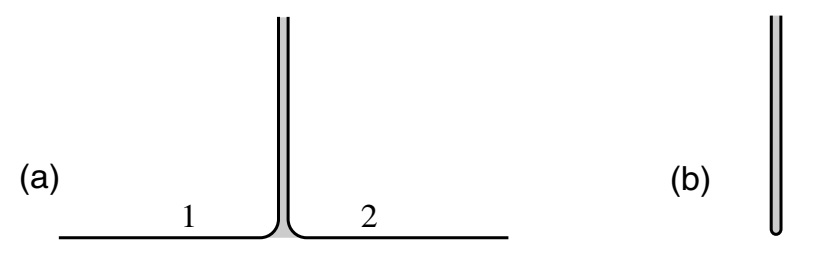
\includegraphics[width=0.8\textwidth]{figure/Fig9.10.jpg}
		\caption{(a) $\Psi_{1} * \Psi_{2}$, the convolution of the right half of $\Psi_{1}$ and the left half of $\Psi_{2}$. This can be considered as defining a path integral for the shaded region, later taking the limit where the width of this region tends to zero. (b) $\int \Psi$, the convolution of the right half and left half of $\Psi$.}\label{Fig9.10}
	\end{center}
\end{figure}
\vspace*{-0.7cm}

There is no problem in solving for interactions. Define the product operation $\Psi_{1} * \Psi_{2}$ on string fields through the functional integral shown in Figure \ref{Fig9.10}a, 
formed by overlapping the right side of $\Psi_{1}$ and the left side of $\Psi_{2}$.
Also define $\int$, which gives the overlap of the right side and left side of a single string wavefunction as shown in Figure \ref{Fig9.10}b. 
To provide an interactive theory, add non-linear terms to the gauge transformation:
\begin{equation}
	\delta \Psi=Q_{\mathrm{B}} \Lambda+g \Psi * \Lambda-g \Lambda * \Psi \:.
	\label{9.6.8}
\end{equation}
The $*$ product is associative, and through a contour discussion, it can be proven that $Q_{\mathrm{B}}$ acts like a derivative:
\begin{equation}
	Q_{\mathrm{B}}(\Psi_{1} * \Psi_{2})=(Q_{\mathrm{B}} \Psi_{1}) * \Psi_{2}+\Psi_{1} *(Q_{\mathrm{B}} \Psi_{2}) \:. \label{9.6.9}
\end{equation}
From these it follows that \eqref{9.6.8} is closed.
Using cyclicity:
\begin{equation}
	\int \Psi_{1} * \Psi_{2}=\int \Psi_{2} * \Psi_{1} \:, \label{9.6.10}
\end{equation}
we can write down the invariant action:
\begin{equation}
	S=\frac{1}{2} \int \Psi * Q_{\mathrm{B}} \Psi + \frac{2 g}{3} \int \Psi * \Psi * \Psi \:.
	\label{9.6.11}
\end{equation}
\begin{tcolorbox}[breakable]
	\begin{remark}
		Conventions (Witten's cubic theory). Signs are graded by ghost number: $\Psi$ is odd, $\Lambda$ is even, and $Q_{\mathrm B}$ is odd. The rules are
		\begin{gather*}
			Q_{\mathrm B}(A*B)=(Q_{\mathrm B}A)*B+(-1)^{|A|}A*(Q_{\mathrm B}B),\\
			\int Q_{\mathrm B}(\cdots)=0,\qquad\int A*B=(-1)^{|A||B|}\int B*A .
		\end{gather*}
		These are the graded forms of \eqref{9.6.9}, of the vanishing of a total BRST variation on the disk, and of \eqref{9.6.10}. To keep track of the relative normalization, write the action as $S=\frac12\int\Psi*Q_{\mathrm B}\Psi+\kappa\int\Psi*\Psi*\Psi$ and the gauge transformation as $\delta\Psi=Q_{\mathrm B}\Lambda+g'(\Psi*\Lambda-\Lambda*\Psi)$.

		\emph{Gauge invariance.} First, $\delta\frac12\int\Psi*Q\Psi=\int\delta\Psi*Q\Psi$ and $\delta\,\kappa\int\Psi^{*3}=3\kappa\int\delta\Psi*\Psi*\Psi$, both by cyclicity. Define $\mathcal I\equiv\int\Lambda*Q\Psi*\Psi-\int\Lambda*\Psi*Q\Psi$. Order by order in the coupling:
		\begin{align*}
			\mathcal O(g^0):&\quad\int Q\Lambda*Q\Psi\eqs{1}\int Q(\Lambda*Q\Psi)=0,\\
			\mathcal O(g^1):&\quad g'\!\int(\Psi*\Lambda-\Lambda*\Psi)*Q\Psi+3\kappa\int Q\Lambda*\Psi*\Psi\eqs{2}g'\,\mathcal I+3\kappa(-\mathcal I)=(g'-3\kappa)\,\mathcal I,\\
			\mathcal O(g^2):&\quad 3\kappa g'\Bigl(\int\Psi*\Lambda*\Psi*\Psi-\int\Lambda*\Psi*\Psi*\Psi\Bigr)\eqs{3}0 .
		\end{align*}
		At (1) $Q^2=0$ and the Leibniz rule were used. At (2) cyclicity gives $\int\Psi*(\Lambda*Q\Psi)=\int\Lambda*Q\Psi*\Psi$, and the Leibniz rule with $\int Q(\Lambda*\Psi*\Psi)=0$ gives $\int Q\Lambda*\Psi*\Psi=-\int\Lambda*Q\Psi*\Psi+\int\Lambda*\Psi*Q\Psi=-\mathcal I$. At (3) the odd $\Psi$ was moved cyclically past $\Lambda*\Psi*\Psi$, which has even degree $0+1+1$, so no sign appears and the two terms cancel. Invariance therefore requires
		\begin{equation*}
			\boxed{g'=3\kappa} .
		\end{equation*}
		With the gauge transformation \eqref{9.6.8} as printed ($g'=g$) the cubic coefficient must be $\kappa=g/3$, which is Witten's normalization $S=\frac12\int\Psi*Q\Psi+\frac g3\int\Psi*\Psi*\Psi$. With the action \eqref{9.6.11} as printed ($\kappa=2g/3$) the gauge transformation must be $\delta\Psi=Q\Lambda+2g(\Psi*\Lambda-\Lambda*\Psi)$. The printed pair is off by a factor of 2 in one of the two places. This is only a normalization of $g$ and does not affect any conclusion.

		\emph{Closure.} Write $[\Psi,\Lambda]\equiv\Psi*\Lambda-\Lambda*\Psi$, so $\delta_\Lambda\Psi=Q\Lambda+g'[\Psi,\Lambda]$. Then
		\begin{align*}
			[\delta_1,\delta_2]\Psi&=g'\bigl([Q\Lambda_1,\Lambda_2]-[Q\Lambda_2,\Lambda_1]\bigr)+g'^2\bigl([[\Psi,\Lambda_1],\Lambda_2]-[[\Psi,\Lambda_2],\Lambda_1]\bigr)\\
			&\eqs{4}Q\bigl(g'[\Lambda_1,\Lambda_2]\bigr)+g'\bigl[\Psi,g'[\Lambda_1,\Lambda_2]\bigr]=\delta_{\Lambda_{12}}\Psi,\qquad\Lambda_{12}=g'[\Lambda_1,\Lambda_2] .
		\end{align*}
		At (4) the Leibniz rule gives $Q[\Lambda_1,\Lambda_2]=[Q\Lambda_1,\Lambda_2]+[\Lambda_1,Q\Lambda_2]$ with $[\Lambda_1,Q\Lambda_2]=-[Q\Lambda_2,\Lambda_1]$, and associativity of $*$ gives the Jacobi identity for the second bracket. So the algebra closes, which is the sense in which \eqref{9.6.8} is ``closed''.
	\end{remark}
\end{tcolorbox}
It is usually useful to write it in CFT form, replacing $\Psi$ with the semi-disk corresponding to the vertex operator $\mathscr{V}_{\Psi}$:
\begin{equation}
	S=\frac{1}{2}\langle\mathscr{V}_{\Psi} \,Q_{\mathrm{B}} \cdot \mathscr{V}_{\Psi}\rangle_{D_{2}} + 
	\frac{2 g}{3}\langle\mathscr{V}_{\Psi} \mathscr{V}_{\Psi} \mathscr{V}_{\Psi}\rangle_{D_{2}} \:. \label{9.6.12}
\end{equation}
The vertex operator positions and conformal coordinates are not as marked in \eqref{9.6.12}, but as shown in Figure \ref{Fig9.11}.
A $z^{2 / 3}$ mapping reshapes the trilinear vertex semi-disk into a disk. 
This action passes a very important test. Only for insertions with a total $Q^{g}=3$, the path integral on the disk is non-zero. The vertex operators for physical states all have ghost number 1, so both terms in \eqref{9.6.12} are non-zero. 
Since \eqref{9.6.11} is invariant, we expect it to reduce to the non-Abelian Yang-Mills action for gauge fields, which indeed it does.


The Siegel gauge is $b_{0} \Psi=0 $.
In the kinetic action, only the $c_{0} L_{0}$ term in $Q_{\mathrm{B}}$ survives. 
Since in components $L_{0} \propto p^{2}+m^{2}$, this is similar to the familiar covariant gauge in electrodynamics.
The propagator:
\begin{equation}
	\int_{0}^{\infty} \dif t \: \exp (-t L_{0}) = L_{0}^{-1} \label{9.6.13}
\end{equation}
\begin{tcolorbox}[breakable]
	\begin{remark}
		Split the BRST charge by ghost zero modes, $Q_{\mathrm B}=c_0L_0+b_0\mathcal M+\hat Q$. Here $\mathcal M$ and $\hat Q$ contain neither $b_0$ nor $c_0$, and $\mathcal M$ is built from $c_{-n}c_n$ with $n\ne0$. In Siegel gauge $b_0\Psi=0$, so $\Psi$ contains no $c_0$. The BPZ product on the disk needs exactly one $c_0$ to saturate the zero mode ($\langle{\downarrow}|c_0|{\downarrow}\rangle\neq0$, $\langle{\downarrow}|{\downarrow}\rangle=0$). Then
		\begin{equation*}
			\lAngle\Psi|Q_{\mathrm B}|\Psi\rangle\eqs{1}\lAngle\Psi|c_0L_0|\Psi\rangle+\lAngle\Psi|\mathcal Mb_0|\Psi\rangle+\lAngle\Psi|\hat Q|\Psi\rangle\eqs{2}\lAngle\Psi|c_0L_0|\Psi\rangle .
		\end{equation*}
		At (1) $b_0\mathcal M=\mathcal Mb_0$, since $b_0$ anticommutes with each $c_{\pm n}$ ($n\ne0$). At (2) the middle term vanishes by $b_0\Psi=0$, and the last one has no $c_0$ at all. The kinetic operator is therefore $c_0L_0$, and on the gauge slice the propagator is $b_0L_0^{-1}$. For $L_0>0$, $L_0^{-1}=\int_0^\infty\dif t\,\me^{-tL_0}$, and elsewhere this is defined by continuation as in \eqref{9.1.22}. Since $L_0$ is the open-string world-sheet Hamiltonian, $\me^{-tL_0}$ is the path integral over a strip of length $t$, and the propagator is the integral over all strip lengths. In components $L_0=\alpha'(k^2+m^2)$, the analogue of Feynman gauge.
	\end{remark}
\end{tcolorbox}
is simply the integral over strips of arbitrary length. The vertex is as shown in Figure \ref{Fig9.11}b where the wedges are removed, and the ends of three strips are inserted into a `$\mathsf{Y}$'.
It has been proven that this is equivalent to the open string theory described by a sum over Riemann surfaces, specifically, this sum includes a complete single-cover of the moduli space. 
On the other hand, this is not unexpected: string field theory has spacetime gauge invariance \eqref{9.6.8}, which makes null states decouple from the S-matrix.
We have argued that the decoupling of null states determines the form of string amplitudes, which includes the requirement for a single-cover of the moduli space (otherwise total derivative terms would give null state coupling). 
On the other hand, moduli space is very complex, and only a few have explicit descriptions. The moduli spaces generated by this string field theory, written as a sum over Feynman diagrams with each diagram being an integral over strip lengths, 
were discovered by physicists only slightly earlier than by mathematicians.\footnote{Another description of moduli space from physics comes from the light-cone gauge, where the moduli are interaction times, 
	the momenta $p^{+}$ of the intermediate states, and the twist angle of each closed string.}


\begin{figure}[!htbp]
	\begin{center}
		%width=0.8\textwidth,bb=0 0 904 352
		%1px=0.75pt
		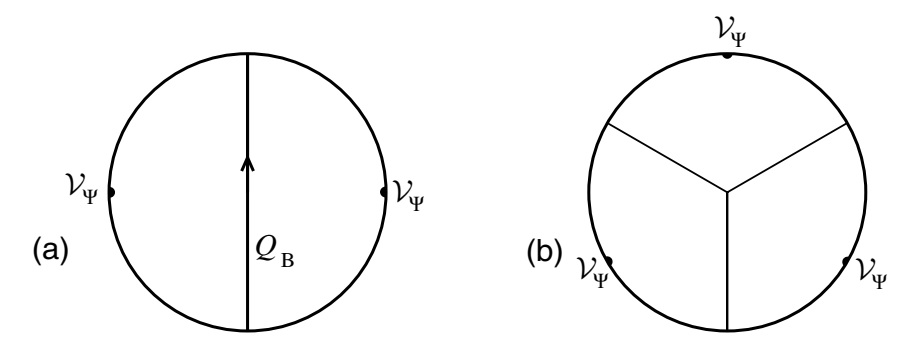
\includegraphics[width=0.8\textwidth]{figure/Fig9.11.jpg}\\
		\caption{CFT representation of the string field action: (a) kinetic term; (b) interaction. A $z^{2/3}$ conformal transformation transforms the usual semi-circle around each vertex operator into the shape of a wedge.}\label{Fig9.11}
	\end{center}
\end{figure}
\vspace*{-0.7cm}

Let's point out a strange feature of this field theory.
We have claimed that string field theory covers the entire moduli space, but we know from the annulus that even without an explicit closed string field, this moduli space will contain the limit that generates closed string poles. 
Closed string poles come from the limit where the strip length tends to zero rather than infinity.\footnote{For this reason, this form of string field theory is not suitable for the purposes of our previous section. We need to add stubs to the vertices to eliminate accidental divergences, 
	and then add closed string propagators and vertices to cover the omitted parts of the moduli space.} The precise statement is that the open string field path integral generates the amplitudes for open string theory plus closed string theory (except for surfaces without any boundaries, which open strings cannot couple to). 
In this sense, in an imprecise way, closed strings are like bound states of open strings.

For theory with only closed strings, we can repeat the above steps with a closed string field, but this will be a bit more complicated. For the free action \eqref{9.6.3}, the ghost number is already insufficient: 
to make matrix elements between physical states non-zero, we need an extra $c$ ghost.
There is a remedy that requires the string field $\Psi$ and gauge transformation $\Lambda$ to be annihilated by $b_{0}-\tilde{b}_{0}$ and $L_{0}-\tilde{L}_{0}$. Then, the action:
\begin{equation}
	S_{0}^{\prime}=\frac{1}{2}\lAngle\Psi |(c_{0}-\tilde{c}_{0}) Q_{\mathrm{B}}| \Psi\rangle \label{9.6.14}
\end{equation}
is invariant under $\delta \Psi=Q_{\mathrm{B}} \Lambda$.
\begin{tcolorbox}[breakable]
	\begin{remark}
		Conventions. Write $b_0^-=b_0-\tilde b_0$, $c_0^-=\frac12(c_0-\tilde c_0)$ and $L_0^-=L_0-\tilde L_0$, so that $\{b_0^-,c_0^-\}=1$ and $\{Q_{\mathrm B},b_0^-\}=L_0^-$. The overall factor of 2 between $c_0-\tilde c_0$ and $c_0^-$ is absorbed in the normalization of $S_0'$. Let $\mathscr H^-$ be the space of states annihilated by $b_0^-$ and $L_0^-$; these states contain no $c_0^-$ excitation.

		\emph{Ghost number.} On the sphere the ghost number must total 6. Closed-string physical fields $\tilde cc\mathscr V$ carry 2, so $\lAngle\Psi|Q_{\mathrm B}|\Psi\rangle$ has $2+1+2=5$ and vanishes identically. The insertion of $c_0^-$ supplies the missing unit: $2+1+1+2=6$.

		\emph{The gauge transformation preserves $\mathscr H^-$.} For $\Lambda\in\mathscr H^-$,
		\begin{equation*}
			L_0^-Q_{\mathrm B}\Lambda=Q_{\mathrm B}L_0^-\Lambda=0,\qquad b_0^-Q_{\mathrm B}\Lambda\eqs{1}\bigl(L_0^--Q_{\mathrm B}b_0^-\bigr)\Lambda=0 ,
		\end{equation*}
		where (1) is $\{Q_{\mathrm B},b_0^-\}=L_0^-$.

		\emph{Invariance.} For $A,B\in\mathscr H^-$ the product $\lAngle A|\mathcal O|B\rangle$ can be nonzero only if $\mathcal O$ contains exactly one $c_0^-$, since neither state does. The operator $\{Q_{\mathrm B},c_0^-\}$ is quadratic in nonzero ghost modes; from $\{Q_{\mathrm B},c_0\}=\sum_mm\,c_mc_{-m}$ and its conjugate, the $m=0$ term vanishes. It therefore contains no $c_0^-$. Then
		\begin{align*}
			\delta S_0'\propto\lAngle Q_{\mathrm B}\Lambda|c_0^-Q_{\mathrm B}|\Psi\rangle
			&\eqs{2}\pm\lAngle\Lambda|Q_{\mathrm B}c_0^-Q_{\mathrm B}|\Psi\rangle
			\eqs{3}\pm\lAngle\Lambda|\bigl(\{Q_{\mathrm B},c_0^-\}-c_0^-Q_{\mathrm B}\bigr)Q_{\mathrm B}|\Psi\rangle\\
			&\eqs{4}\pm\lAngle\Lambda|\{Q_{\mathrm B},c_0^-\}|Q_{\mathrm B}\Psi\rangle\eqs{5}0 .
		\end{align*}
		At (2) $Q_{\mathrm B}$ was moved to the other side of the BPZ product. At (3) the anticommutator was introduced. At (4) $Q_{\mathrm B}^2=0$. At (5) both $\Lambda$ and $Q_{\mathrm B}\Psi$ lie in $\mathscr H^-$ and the operator has no $c_0^-$. The same argument shows that the quadratic form is symmetric, so varying $\Psi$ again gives the equation of motion $Q_{\mathrm B}\Psi=0$ on $\mathscr H^-$. This is precisely the closed-string BRST condition, together with the conditions $(b_0-\tilde b_0)\Psi=(L_0-\tilde L_0)\Psi=0$ of the closed-string BRST analysis in Chapter \ref{cha:4}.
	\end{remark}
\end{tcolorbox}
For an interaction theory, there is no longer an associative product similar to $*$, and correspondingly no single-cover of the moduli space. 
As in the previous section, to cover the moduli space, we need to add higher order vertices $\mathscr{V}_{g, n}$ with higher powers of the field and internal handles. 
Similar to the open string action, the corresponding action can be derived from symmetry principles using the so-called Batalin-Vilkovisky formalism. Then, gauge fixing gives the perturbation theory described in the previous section.

The derivation of string theory from spacetime gauge symmetry is extremely elegant, especially for open strings. Introducing closed strings into open string field theory is very appealing. However, it is not yet known whether string field theory is a useful tool beyond perturbation theory. 
In contemporary non-perturbative developments based on spacetime supersymmetry, string field theory has played no role, and such developments will be discussed in Chapter 14.
It is quite possible that for the non-perturbative construction of ``string theory,'' strings, or string fields, are simply not its correct degrees of freedom.

\section{Large order behavior} \label{sec:9.7}

There is an interesting result about the large order behavior of string perturbation theory. We start with field theory.
Consider the integral:
\begin{equation}
	\int_{-\infty}^{\infty} \dif y \exp \biggl[-\frac{y^{2}}{2!} - \lambda \frac{y^{3}}{3!}\biggr] = 
	\lambda^{-1} \int_{-\infty}^{\infty} \dif z \exp \biggl[-\frac{1}{\lambda^{2}}\biggl(\frac{z^{2}}{2!}+\frac{z^{3}}{3!}\biggr)\biggr] \:,
	\label{9.7.1}
\end{equation}
where $z=y \lambda $.
This integral diverges for $\lambda \neq 0$, but we ignore it for now and compute it as a formal power series in $\lambda$:
\begin{equation}
	\sum_{n=0}^{\infty} \frac{(-\lambda)^{n}}{6^{n} n !} \int_{-\infty}^{\infty} \dif y\: y^{3 n} 
	\exp (-y^{2} / 2) = (2 \pi)^{1 / 2} \sum_{k=0}^{\infty} \lambda^{2 k} C_{2 k} \:, \label{9.7.2}
\end{equation}
where:
\begin{equation}
	C_{2 k}=\frac{2^{k} \Gamma(3 k+1 / 2)}{\pi^{1 / 2} 3^{2 k}(2 k) !} \:.
	\label{9.7.3}
\end{equation}
\begin{tcolorbox}[breakable]
	\begin{remark}
		\emph{Rescaling \eqref{9.7.1}.} With $y=z/\lambda$, $\frac{y^2}{2}+\lambda\frac{y^3}{6}=\frac{1}{\lambda^2}\bigl(\frac{z^2}{2}+\frac{z^3}{6}\bigr)$ and $\dif y=\dif z/\lambda$. So the coupling appears only as an overall $1/\lambda^2$, like $1/\hbar$.

		\emph{Coefficients.} Expand $\exp(-\lambda y^3/6)$ and use $\int\dif y\,y^{2m}\me^{-y^2/2}=2^{m+1/2}\Gamma(m+\frac12)$. Only even powers survive:
		\begin{align*}
			\sum_{n}\frac{(-\lambda)^n}{6^nn!}\int\dif y\,y^{3n}\me^{-y^2/2}
			&\eqs{1}\sum_k\frac{\lambda^{2k}}{6^{2k}(2k)!}\,2^{3k+1/2}\,\Gamma\bigl(3k+\tfrac12\bigr)\\
			&\eqs{2}(2\pi)^{1/2}\sum_k\lambda^{2k}\,\frac{2^{3k}\Gamma(3k+\frac12)}{\pi^{1/2}\,2^{2k}3^{2k}(2k)!} ,
		\end{align*}
		which is \eqref{9.7.3} after $2^{3k}/2^{2k}=2^k$. At (1) odd $n$ vanish by parity, and $n=2k$ gives $m=3k$. At (2) $2^{1/2}=(2\pi)^{1/2}/\pi^{1/2}$ and $6^{2k}=2^{2k}3^{2k}$.

		\emph{Check at $k=1$.} $C_2=\frac{2\,\Gamma(7/2)}{\pi^{1/2}\cdot9\cdot2}=\frac{15/8}{9}=\frac{5}{24}$, using $\Gamma(7/2)=\frac{15}{8}\pi^{1/2}$. The two vacuum graphs with two cubic vertices are the ``theta'' graph (two vertices joined by three lines) and the ``dumbbell'' (two tadpoles joined by a line). Their automorphism groups have orders $2\cdot3!=12$ and $2\cdot2\cdot2=8$, and $\frac1{12}+\frac18=\frac{5}{24}$.
	\end{remark}
\end{tcolorbox}
This integral is the zero-dimensional limit of scalar field theory with a mass term and cubic coupling. The expansion in $\lambda$ can be represented as Feynman diagrams, where the propagator of the diagram is 1 and the vertex is $-\lambda$. 
Thus the constant $C_{2 k}$ counts the total number of vacuum diagrams with $2k$ three-point vertices, which is equivalently the total number of vacuum diagrams with $k+1$ loops, each assigned an appropriate symmetry factor.
For example, the reader can verify that there are two vacuum diagrams with two vertices, with symmetry group orders of 8 and 12, respectively, and $C_{2}=\frac{5}{24}=\frac{1}{8}+\frac{1}{12}$. 
To get the large order behavior, we use Stirling's approximation $n ! \approx n^{n+1 / 2} \me^{-n}$, then:
\begin{equation}
	C_{2 k} \approx k^{k} \approx k !
	\:, \label{9.7.4}
\end{equation}
where the approximation holds up to a factor of the form $k^{a}$ and $b^{k}$.
\begin{tcolorbox}[breakable]
	\begin{remark}
		Stirling's formula $\Gamma(x+1)\approx x^x\me^{-x}$ (dropping powers of $x$) gives
		\begin{equation*}
			C_{2k}\approx\frac{2^k(3k)^{3k}\me^{-3k}}{9^k(2k)^{2k}\me^{-2k}}\eqs{1}\Bigl(\frac{2\cdot27}{9\cdot4}\Bigr)^kk^k\me^{-k}=\Bigl(\frac32\Bigr)^kk^k\me^{-k}\eqs{2}\Bigl(\frac32\Bigr)^k\Gamma(k) .
		\end{equation*}
		At (1) the powers of $k$ and the numerical factors were collected. At (2) $k^k\me^{-k}\approx\Gamma(k)$, again up to powers. So $C_{2k}\approx k!\,b^k$ with $b=\frac32$. The base $b$ has a meaning: the stationary points of $S(z)=\frac{z^2}{2}+\frac{z^3}{6}$ are $z=0$ and $z=-2$, where $S(-2)=2-\frac86=\frac23$. The instanton action is $S(-2)/\lambda^2=2/3\lambda^2$, and the large-order growth is $C_{2k}\sim\Gamma(k)\,[S(-2)]^{-k}$, with $1/S(-2)=\frac32$ exactly the base found above.
	\end{remark}
\end{tcolorbox}

We can also introduce a quartic term $\lambda^{2} y^{4} / 4 !$, which makes the integral converge. The power of $\lambda$ is decided by requiring all terms in the action for $z$ to be proportional to $\lambda^{-2}$; 
or equivalently, all $k+1$ loop vacuum diagrams are assigned a weight $\lambda^{2k}$.
This extra term does not change the result substantially; the estimate \eqref{9.7.4} still holds within certain accuracy.

When considering field theory, propagators and vertices become more complicated. However, the dominant behavior at large orders often comes from the counting of diagrams—unless there is unusual IR or UV behavior, propagators and vertices usually contribute a factor of order $b^{k}$. 
The series takes the following form:
\begin{equation}
	\sum_{k=0}^{\infty} \lambda^{2 k} k !
	f_{2 k} \:, \label{9.7.5}
\end{equation}
where $f_{2 k} \approx k^{a} b^{k}$, which changes much slower than $k!$. Unless there is unexpected cancellation in $f_{2 k}$, this diverges.
For very small $\lambda$, this will be small temporarily, then grow like $k!$. The order of the smallest term in the sum is:
\begin{equation}
	\exp [-O(1 / \lambda^{2})] \:. \label{9.7.6}
\end{equation}
\begin{tcolorbox}[breakable]
	\begin{remark}
		Take $a_k=\lambda^{2k}k!\,f_{2k}$ with $f_{2k}\approx b^k$ (powers of $k$ do not change the estimate). The ratio of successive terms is
		\begin{equation*}
			\frac{a_{k+1}}{a_k}\approx b\lambda^2(k+1)\quad\Longrightarrow\quad a_k\text{ decreases until }k_*\approx\frac{1}{b\lambda^2},
		\end{equation*}
		and the smallest term is
		\begin{equation*}
			a_{k_*}\approx(b\lambda^2)^{k_*}k_*!\eqs{1}(b\lambda^2k_*)^{k_*}\me^{-k_*}\eqs{2}\exp\Bigl(-\frac{1}{b\lambda^2}\Bigr) .
		\end{equation*}
		At (1) Stirling was used. At (2) $b\lambda^2k_*=1$. Truncating the series at its smallest term therefore leaves an irreducible uncertainty of this order. For the example above, $b=\frac32$ gives $\me^{-2/3\lambda^2}$, which is $\me^{-S_{\text{inst}}}$.
	\end{remark}
\end{tcolorbox}
This is the feature of an asymptotic expansion where the accuracy of perturbation theory is limited. Indeed, effects like instantons or dynamical symmetry breaking, which are zero to all orders in perturbation theory, are generally of this order.
For example, the large order behavior of the series \eqref{9.7.2} is related to the instanton (stable point) at $z=-2$, and the instanton action is $2 / 3 \lambda^{2}$.

In string theory, the Feynman diagrammatic decomposition of the moduli space makes it entirely possible to construct the same constraints. For a series of the form \eqref{9.7.5}, where $f_{2 k}$ is positive-definite and has a lower bound $b^{k}$, this has been explicitly proven.
Thus, this series is divergent and not even Borel summable. Borel summation rewrites the series \eqref{9.7.5} as a Laplace transform of another more convergent series:
\begin{equation}
	\int_{0}^{\infty} \dif t\: \exp (-t) \sum_{k=0}^{\infty}(t \lambda^{2})^{k} f_{2 k} \:. \label{9.7.7}
\end{equation}
However, the positive-definiteness of $f_{2 k}$ implies that this new sum, even if convergent, has poles on the positive real axis, so this integral is ill-defined.
\begin{tcolorbox}[breakable]
	\begin{remark}
		The equality of \eqref{9.7.5} and \eqref{9.7.7} term by term is $\int_0^\infty\dif t\,\me^{-t}t^k=k!$. For the model growth $f_{2k}=b^k$,
		\begin{equation*}
			\sum_k(t\lambda^2)^kb^k=\frac{1}{1-b\lambda^2t},
		\end{equation*}
		which has a pole at $t_*=1/b\lambda^2>0$, on the integration contour. Positive $f_{2k}$ always put the nearest singularity on the positive axis. Passing the pole above or below gives results that differ by $2\pi\mi$ times the residue,
		\begin{equation*}
			\Delta=\pm2\pi\mi\,\frac{\me^{-t_*}}{b\lambda^2}=\pm\frac{2\pi\mi}{b\lambda^2}\exp\Bigl(-\frac{1}{b\lambda^2}\Bigr),
		\end{equation*}
		an ambiguity of exactly the size \eqref{9.7.6} of the smallest term. The perturbation series alone does not fix these $\exp[-O(1/\lambda^2)]$ terms.
	\end{remark}
\end{tcolorbox}
Thus, we expect an interesting non-perturbative phenomenon in string theory. This is not surprising since they degenerate to non-trivial field theories in the low-energy limit.

The estimate \eqref{9.7.4} is a lower bound for closed string theory, which can be obtained by only keeping the tree-level trilinear vertex $\mathscr{V}_{0,3}$. 
Since closed string vertices will receive corrections from Riemann surfaces of all genus, we wonder if the perturbation theory will grow even faster. One way to see that it does is to recall that open string field theory contains all open string Riemann surfaces, 
and closed string Riemann surfaces with at least one boundary. Let's examine surfaces with only one boundary, and the moduli space region where the boundary shrinks to a point. 
The limit of the open string moduli space equals the moduli space of a closed surface with one vertex operator. It can be proven that this region is not much smaller than the entire open string moduli space, so the same estimate still holds.
The perturbation series tends to:
\begin{equation}
	\sum_{k=0}^{\infty} g_{\mathrm{o}}^{2 k} O(k !)=\sum_{k=0}^{\infty} g_{\mathrm{c}}^{k} O(k !) \:. \label{9.7.8}
\end{equation}
The term of genus $g$ is proportional to $g_{\mathrm{c}}^{2 g}$, and it has a coefficient of order $(2g)!$.
This is larger than the $g!$ feature of field theory, 
which is also the lower bound obtained only from $\mathscr{V}_{0,3}$. Clearly, the largest part of the high-order amplitudes is contained in the vertex $\mathscr{V}_{g, n}$ and comes from the interior of the moduli space. 
Non-perturbative effects can be expected to be of the order:
\begin{equation}
	\exp [-O(1/g_{\mathrm{c}})] \:, \label{9.7.9}
\end{equation}
\begin{tcolorbox}[breakable]
	\begin{remark}
		Each open-string loop costs $g_{\mathrm o}^2$ and each handle $g_{\mathrm o}^4\propto g_{\mathrm c}^2$, so $g_{\mathrm o}^{2k}=g_{\mathrm c}^{k}$ up to constants, which is \eqref{9.7.8}. Genus $g$ then corresponds to $k=2g$, with coefficient $(2g)!$. Repeating the estimate of \eqref{9.7.6} with $a_k=g_{\mathrm c}^k\,k!\,b^k$:
		\begin{equation*}
			\frac{a_{k+1}}{a_k}\approx bg_{\mathrm c}(k+1)\ \Rightarrow\ k_*\approx\frac{1}{bg_{\mathrm c}},\qquad a_{k_*}\approx(bg_{\mathrm c}k_*)^{k_*}\me^{-k_*}=\exp\Bigl(-\frac{1}{bg_{\mathrm c}}\Bigr).
		\end{equation*}
		The only change from field theory is that $g_{\mathrm c}$ replaces $\lambda^2\sim g_{\mathrm c}^2$ as the expansion parameter multiplying $k!$. So the ambiguity is $\me^{-O(1/g_{\mathrm c})}$, parametrically larger than the field-theory $\me^{-O(1/g_{\mathrm c}^2)}$ at weak coupling.
	\end{remark}
\end{tcolorbox}
which is much larger than the field theory feature $\exp[-O(1 / g_{\mathrm{c}}^{2})]$ at weak coupling. The large order behavior was first observed in some simplified models discussed in Section \ref{sec:9.9}.
We will see in Chapter 13 that these effects are related to D-branes, at least in some superstring theories.


\section{High energy and high temperature} \label{sec:9.8}

To gain a better understanding of string dynamics, we can look at its behavior in different limits. In this section, we examine various high-energy limits of string theory.

\subsection*{Hard scattering}

Again, examine the hard scattering behavior, which is obtained by applying Stirling's approximation to the Veneziano and Virasoro-Shapiro amplitudes.
Returning to the integral form \eqref{6.6.5}:
\begin{equation}
	\frac{8 \pi \mi g_{\mathrm{c}}^{2}}{\alpha^{\prime}} (2\pi)^{26} \delta^{26}({\textstyle \sum_{i} k_{i}}) 
	\int_{\mathds{C}} \dif^{2} z_{4} \: |z_{4}|^{-\alpha^{\prime}u/2 - 4}|1-z_{4}|^{-\alpha^{\prime} t/2 - 4} \:.
	\label{9.8.1}
\end{equation}
In the hard scattering region where $t/s$ is kept fixed and $s \rightarrow \infty$, the exponent is very large, and the integral is dominated by the stationary point of the exponent.\footnote{As usual, the integral diverges as $z_{4}\to \infty$ and is defined by analytic continuation. The reasonableness of the saddle point approximation can be argued by continuation.} When $s, t, u \gg 1$, the saddle point is:
\begin{equation}
	\frac{\partial}{\partial z_{4}}\Bigl(u \ln |z_{4}|^{2}+t \ln |1-z_{4}|^{2}\Bigr) = 
	\frac{u}{z_{4}} + \frac{t}{z_{4}-1} = 0 \:, \label{9.8.2}
\end{equation}
its solution is $z_{4} = -u/s$;
recall that $s+t+u=O(1)$. Then the saddle point approximation gives the amplitude:
\begin{equation}
	S \approx \exp [-\alpha^{\prime}(s \ln s + t \ln t + u \ln u) / 2] \:, \label{9.8.3}
\end{equation}
the same as given by \eqref{6.6.13}.
\begin{tcolorbox}[breakable]
	\begin{remark}
		For large $s,t,u$ the $-4$'s in the exponents of \eqref{9.8.1} are subleading, and the integrand is $\me^{E(z,\bar z)}$ with
		\begin{equation*}
			E=-\frac{\alpha'}{4}\Bigl(u\ln|z|^2+t\ln|1-z|^2\Bigr).
		\end{equation*}
		\emph{Saddle point.} Setting $\partial_zE=0$,
		\begin{equation*}
			\frac uz+\frac{t}{z-1}=0\;\Longrightarrow\;u(z-1)+tz=0\;\Longrightarrow\;z_*=\frac{u}{u+t}\eqs{1}-\frac us ,\qquad 1-z_*=\frac{s+u}{s}\eqs{1}-\frac ts .
		\end{equation*}
		At (1) $s+t+u=O(1)$ is negligible, so $u+t\approx-s$.

		\emph{Value.} Substituting,
		\begin{align*}
			E(z_*)&=-\frac{\alpha'}{4}\Bigl(u\ln\frac{u^2}{s^2}+t\ln\frac{t^2}{s^2}\Bigr)
			=-\frac{\alpha'}{2}\Bigl(u\ln|u|+t\ln|t|-(u+t)\ln s\Bigr)\\
			&\eqs{2}-\frac{\alpha'}{2}\Bigl(s\ln s+t\ln|t|+u\ln|u|\Bigr),
		\end{align*}
		with (2) again $-(u+t)=s$. This is \eqref{9.8.3}. The Gaussian integral around the saddle and the imaginary parts of the logarithms (for $t,u<0$) affect only the prefactor and the phase, not the exponential falloff of $|S|$.
	\end{remark}
\end{tcolorbox}
Let us step back and move from the integral over $z_{4}$ back to the path integral over $X^{\mu}$. It is dominated by the saddle point:
\begin{equation}
	X_{\mathrm{cl}}^{\mu}(\sigma) = \mi \sum_{i} k_{i}^{\mu} G^{\prime}(\sigma, \sigma_{i}) \:, \label{9.8.4}
\end{equation}
where $\sigma_{i}$ is the vertex operator position. Recall that the Green's function is proportional to $\alpha^{\prime}$.
At high energy, the size of the scattering region grows linearly with energy, $\delta X \approx \alpha^{\prime} k$. 
In field theory, high-energy hard scattering probes small distances through the uncertainty principle, $\delta X \approx 1 / k$. In string theory, this is not the case once the string scale is exceeded. 
In string perturbation theory, it manifests as the impossibility of probing distances smaller than this scale, giving the concept that it is the limiting distance in spacetime.
The effective lower bound $R \approx \alpha^{\prime 1/2}$ on compactification also supports this point. However, we will see in Chapter 13 that some recent developments in non-perturbative string theory reveal the existence of even lower distance scales.

In the general order of string loop expansion, the dominant term in the amplitude is:
\begin{equation}
	\exp \Biggl[-\sum_{i<j} k_{i} \cdot k_{j} G^{\prime}(\sigma_{i}, \sigma_{j})\Biggr] \:.
	\label{9.8.5}
\end{equation}
\begin{tcolorbox}[breakable]
	\begin{remark}
		Conventions (Section \ref{sec:6.2}). $S=\frac{1}{4\pi\alpha'}\int\dif^2\sigma\,\partial_aX\cdot\partial_aX$, and the Green's function obeys $-\frac{1}{2\pi\alpha'}\nabla^2G'(\sigma,\sigma')=\delta^2(\sigma-\sigma')$ up to the zero-mode subtraction. On the sphere $G'=-\frac{\alpha'}{2}\ln|z-z'|^2+\cdots$. The vertex operators act as a source, $\prod_i\me^{\mi k_i\cdot X(\sigma_i)}=\exp\int J\cdot X$ with $J(\sigma)=\mi\sum_ik_i\delta^2(\sigma-\sigma_i)$.

		\emph{Saddle \eqref{9.8.4}.} Varying $-S+\int J\cdot X$,
		\begin{gather*}
			\frac{1}{2\pi\alpha'}\nabla^2X+J=0\\
			\Longrightarrow\;X_{\mathrm{cl}}(\sigma)=\int\dif^2\sigma'\,G'(\sigma,\sigma')J(\sigma')=\mi\sum_ik_iG'(\sigma,\sigma_i) .
		\end{gather*}
		\emph{Exponent \eqref{9.8.5}.} Integrating by parts, $S[X_{\mathrm{cl}}]=\frac{1}{4\pi\alpha'}\int X_{\mathrm{cl}}(-\nabla^2X_{\mathrm{cl}})=\frac12\int J\cdot X_{\mathrm{cl}}$. So
		\begin{align*}
			-S+\int J\cdot X\Bigr|_{\mathrm{cl}}&=\frac12\int J\cdot X_{\mathrm{cl}}\eqs{1}\frac12\sum_{i,j}(\mi k_i)\cdot(\mi k_j)G'(\sigma_i,\sigma_j)\\
			&=-\sum_{i<j}k_i\cdot k_jG'(\sigma_i,\sigma_j)-\frac12\sum_ik_i^2G'_{\mathrm r}(\sigma_i,\sigma_i) .
		\end{align*}
		At (1) the solution was inserted. The diagonal terms are the renormalized self-contractions, which normal ordering removes; they are in any case small compared with the $k_i\cdot k_j$, since $k_i^2=-m_i^2$ stays fixed while $k_i\cdot k_j\sim s$. The exponent is Gaussian in $X$, so the fluctuations about $X_{\mathrm{cl}}$ give a $k$-independent determinant and the saddle point is exact here. On the sphere this reproduces $\prod_{i<j}|z_{ij}|^{\alpha'k_i\cdot k_j}$. Since $G'\propto\alpha'$, $X_{\mathrm{cl}}\sim\alpha'k$, the growth of the interaction region noted in the text.
	\end{remark}
\end{tcolorbox}
We need to find the saddle point of this exponent: both for the position of the vertex operator and the modulus of the Riemann surface. This is very much like an electrostatics problem: 
the exponent is the energy of $n$ particles with charge $k_{i}^{\mu}$ on a Riemann surface, where $\mu$ marks $d$ different electrostatic fields, and $\mu=0$ has the opposite sign in energy. 
The background charge density is zero due to momentum conservation, and since $k_{i}^{2}$ is on-shell and very small, the renormalized self-energy can be neglected.
Quite remarkably, at every genus, a possible saddle point is found. Consider a Riemann surface:
\begin{equation}
	z_{2}^{N} = \frac{(z_{1}-a_{1})(z_{1}-a_{2})}{(z_{1}-a_{3})(z_{1}-a_{4})} \:. \label{9.8.6}
\end{equation}
Like the hyperelliptic curve \eqref{9.2.9}, it is a subspace of $S_{2} \times S_{2}$. It can be viewed as $N$ sheets glued at the branch cuts and has genus $N{-}1$.
For four-point amplitudes, if the charges are located at the branch cuts $a_{i}$, the amplitude is stable relative to their positions—the surface is ``vertical'' at these points, $\partial z_{2} / \partial z_{1}=\infty$, 
and the symmetry $z_{2} \to \exp (2 \pi \mi / N) z_{2}$ requires the vertical component of the gradient to be zero.
It remains an extremum relative to the position $a_{i}$, but this is easy: 
the electric field is the same as that of a charge at $z=a_{i}$ on the sphere, except that it is split into $N$ branch sheets. Thus the energy is $N \cdot N^{-2}=N^{-1}$ times the energy on the sphere, 
where three positions can be fixed to $0,1,\infty$ by Möbius transformation, and the fourth is given by the condition on the sphere \eqref{9.8.2}.
Thus at genus $g$,
\begin{equation}
	S_{g} \approx \exp [-\alpha^{\prime}(s \ln s + t \ln t + u \ln u) / 2(g+1)] \:.
	\label{9.8.7}
\end{equation}
\begin{tcolorbox}[breakable]
	\begin{remark}
		\emph{Genus of \eqref{9.8.6}.} The projection $(z_1,z_2)\mapsto z_1$ is $N$-sheeted. Near $a_1$, $z_2^N\propto(z_1-a_1)$, so all $N$ sheets meet (ramification index $N$) and $z_2$ is a good local coordinate. The same holds at $a_2$, and at $a_3,a_4$ where $z_2\to\infty$. At $z_1=\infty$ the right side tends to $1$, giving $N$ distinct points, so there is no branching. Riemann--Hurwitz gives
		\begin{equation*}
			2-2g=N\cdot2-4(N-1)=4-2N\quad\Longrightarrow\quad g=N-1 .
		\end{equation*}
		\emph{Energy.} Let $\hat a_i$ be the single preimage of $a_i$. The potential $\phi_i$ of a unit charge at $\hat a_i$ is invariant under $z_2\to\me^{2\pi\mi/N}z_2$, because that map fixes $\hat a_i$. So $\phi_i$ is the pullback of a function $f_i$ on the $z_1$-sphere. The equation $\nabla^2\phi=$ (source) is conformally invariant in two dimensions, so away from the branch points $\nabla^2\phi_i$ is the pullback of $\nabla^2f_i$. Its total flux, summed over the $N$ sheets, is $N$ times that of $f_i$, while the source on $M$ has unit strength. Hence $f_i$ has source $1/N$:
		\begin{equation*}
			G'_M(\hat a_i,\hat a_j)=\frac1N\,G'_{S_2}(a_i,a_j)\quad\Longrightarrow\quad\sum_{i<j}k_i\cdot k_jG'_M(\hat a_i,\hat a_j)=\frac{1}{N}\sum_{i<j}k_i\cdot k_jG'_{S_2}(a_i,a_j).
		\end{equation*}
		The constant zero-mode pieces drop out by momentum conservation. This is the ``$N\cdot N^{-2}$'' of the text: the field on each sheet is $1/N$ of the sphere field, and there are $N$ sheets. Because the exponent is proportional to the sphere's, its stationary point in the $a_i$ is the sphere's, $z_4=-u/s$. By \eqref{9.8.3}, $\ln S_g\approx\frac{1}{N}\ln S_0$ with $N=g+1$, which is \eqref{9.8.7}. Likewise $X_{\mathrm{cl}}\propto G'$ is divided by $N$.
	\end{remark}
\end{tcolorbox}
With extra effort, Gaussian fluctuations near the saddle point can be introduced, which determine the coefficient of $S_{g}$. For the $N$-branched saddle point, $X_{\mathrm{cl}}^{\mu}$ only needs to be divided by $N=g{+}1$.

There is a way to test if this result is indeed reasonable. In the small-angle region $-t / s \ll 1$, it becomes:
\begin{equation}
	\exp [\alpha^{\prime} t \ln s / 2(g+1)] \:.
	\label{9.8.8}
\end{equation}
Now $t^{1 / 2}$ is the total transferred momentum from incident particle 1 to final state particle 3. In the small-angle region, the scattering process with genus $g$ appears to be decomposed into $g{+}1$ successive scatterings. 
Each scattering has the same center of mass $s$, while $t_{i}$ must satisfy the constraint that the total transferred momentum is $t^{1/2}$.
A single scattering tends to $\exp (\alpha^{\prime} t_{i} \ln s / 2)$. 
Then it is easily verified that taking the momentum transfers to be equal is most efficient, i.e., $t_{i}^{1/2}=t^{1/2} /(g+1)$, which gives the result of the product of amplitudes \eqref{9.8.8}. 
This is different from particle scattering, where the most effective scattering process is transferring momentum to a few hard scatterings.
\begin{tcolorbox}[breakable]
	\begin{remark}
		\emph{Small-angle limit.} For $|t|\ll s$ with $t<0$, $u=-s-t$ and $|u|=s+t$ (using $s+t+u\approx0$). Then
		\begin{align*}
			s\ln s+t\ln|t|+u\ln|u|&=s\ln s+t\ln|t|-(s+t)\ln(s+t)\\
			&\eqs{1}s\ln s+t\ln|t|-(s+t)\Bigl(\ln s+\frac ts\Bigr)+\cdots\\
			&=-t\ln s+t\ln|t|-t+\cdots\eqs{2}-t\ln s .
		\end{align*}
		At (1) $\ln(s+t)=\ln s+t/s+\cdots$. At (2) only the term enhanced by $\ln s$ was kept. Inserting into \eqref{9.8.7} gives $\exp[\alpha't\ln s/2(g+1)]$, which is \eqref{9.8.8}.

		\emph{Successive scatterings.} Let $q_i=\sqrt{-t_i}\ge0$ be the momentum transfers of $g+1$ collinear small-angle scatterings, with $\sum_iq_i=q=\sqrt{-t}$. The product of single-scattering amplitudes is $\exp\bigl(-\frac{\alpha'}{2}\ln s\sum_iq_i^2\bigr)$. It is largest when $\sum_iq_i^2$ is smallest at fixed $\sum_iq_i$, which by Cauchy--Schwarz is at $q_i=q/(g+1)$:
		\begin{equation*}
			\sum_iq_i^2\ge\frac{(\sum_iq_i)^2}{g+1}=\frac{q^2}{g+1}\quad\Longrightarrow\quad\prod_i\me^{\alpha't_i\ln s/2}\le\exp\Bigl[\frac{\alpha't\ln s}{2(g+1)}\Bigr],
		\end{equation*}
		and the bound is attained at equal transfers. This reproduces \eqref{9.8.8}.
	\end{remark}
\end{tcolorbox}

For string excited states, the exponential behavior of the vertex operator is the same as the tachyon. Then the dominant behavior is the same saddle point, and $X_{\mathrm{cl}}^{\mu}$ is substituted into the vertex operator.
Since except for a $g+1$ factor, the dominant saddle point is the same for all states and all orders, there exists a linear relationship between the scatterings of different states, which holds for all genus and thus is very likely to hold for exact amplitudes. 
In quantum field theory, high-energy scattering usually reveals symmetries that are not obvious at low energy. It is widely agreed that the relationship found here belongs to the same category.

It is still unclear under what circumstances the sum of the series \eqref{9.8.7} is meaningful. It makes sense to compare this section with the results of the previous section. 
In both cases, it is the interior of the moduli space that produces interesting physical results (in contrast, field theory behavior occurs at the boundary). 
However, high-order behavior comes from the entire moduli space, in particular, this behavior is dominated by the large volume of the moduli space. High-energy behavior at a fixed genus is dominated by a single point.

\subsection*{Regge scattering}

The analysis of the Regge limit can also be extended to higher orders. We will not do this, but we will develop an interesting explanation of tree-level Regge physics.
For most physicists, Regge scattering is not as familiar as hard scattering. It is a gentle probe of high-velocity systems. 
When a system is boosted, time dilation slows down its internal processes. Thus, when a high-energy system tends to high energy, we can expect to see more virtual degrees of freedom.

Let's examine the quantum fluctuations of a single string, its square root meaning the scale of the ground state. The mode expansion gives:
\begin{align}
	\langle 0 |[X^{1}(\sigma)-x^{1}]^{2}|
	0\rangle &= \sum_{n=1}^{\infty} \frac{\alpha^{\prime}}{2 n^{2}}
	\langle 0|(\alpha_{n} \alpha_{-n} + \tilde{\alpha}_{n} \tilde{\alpha}_{-n})| 0\rangle  \nonumber \\
	&= \alpha^{\prime} \sum_{n=1}^{\infty} \frac{1}{n} \:. \label{9.8.9}
\end{align}
This is divergent, but has no significant physical meaning.
\begin{tcolorbox}[breakable]
	\begin{remark}
		Take the closed-string expansion at fixed $\tau$ with the zero-mode momentum dropped (the ground state at rest):
		\begin{equation*}
			X^1(\sigma)-x^1=\mi\Bigl(\frac{\alpha'}{2}\Bigr)^{1/2}\sum_{n\ne0}\frac1n\bigl(\alpha^1_n\me^{-\mi n(\tau-\sigma)}+\tilde\alpha^1_n\me^{-\mi n(\tau+\sigma)}\bigr) .
		\end{equation*}
		In $\langle0|(\cdots)^2|0\rangle$ only $\alpha_n\alpha_{-n}$ and $\tilde\alpha_n\tilde\alpha_{-n}$ with $n>0$ survive: $\alpha_{-n}$ and $\tilde\alpha_{-n}$ annihilate $\langle0|$, $\alpha_n$ and $\tilde\alpha_n$ annihilate $|0\rangle$, and left-right cross terms vanish. For such a pair the factor is $\mi^2\cdot\frac{1}{n}\cdot\frac{1}{(-n)}=\frac{1}{n^2}$, and the phases cancel. With $[\alpha^1_n,\alpha^1_{-n}]=n$,
		\begin{equation*}
			\langle0|[X^1-x^1]^2|0\rangle=\frac{\alpha'}{2}\sum_{n=1}^\infty\frac{1}{n^2}\langle0|\alpha_n\alpha_{-n}+\tilde\alpha_n\tilde\alpha_{-n}|0\rangle=\frac{\alpha'}{2}\sum_{n\ge1}\frac{2n}{n^2}=\alpha'\sum_{n\ge1}\frac1n ,
		\end{equation*}
		which is \eqref{9.8.9}. If only modes with $n\lesssim n_{\max}=\alpha'^{1/2}/\delta\tau$ are resolved, $\sum_{n\le n_{\max}}1/n\approx\ln n_{\max}$ and the mean square size is $\alpha'\ln(\alpha'^{1/2}/\delta\tau)$.
	\end{remark}
\end{tcolorbox}
Measurement at time scale $\delta \tau$ is only sensitive to modes with frequency less than $\delta \tau^{-1}$, 
and again $n \alpha^{\prime-1 / 2}<\delta \tau^{-1}$. The logarithmic divergence becomes $\alpha^{\prime} \ln(\alpha^{\prime 1/2} / \delta\tau)$, and the size is its square root.
The growth of the effective size is directly observable in the Regge amplitude \eqref{6.6.12} with very small $t$:
\begin{equation}
	s^{2+\alpha^{\prime}t/2} \frac{\Gamma(-\alpha^{\prime} t/4 - 1)}{\Gamma(\alpha^{\prime} t/4 + 2)} \sim 
	\frac{s^{2}}{t} \exp \biggl[-\frac{q^{2} \alpha^{\prime}}{2} \ln (\alpha^{\prime} s)\biggr] \:, \label{9.8.10}
\end{equation}
where $q^{2}=-t$ is the momentum transfer.
\begin{tcolorbox}[breakable]
	\begin{remark}
		For $|t|\ll1/\alpha'$ put $\varepsilon=-\alpha't/4\to0^+$. Then
		\begin{equation*}
			\Gamma\Bigl(-\frac{\alpha't}{4}-1\Bigr)=\Gamma(\varepsilon-1)\eqs{1}\frac{\Gamma(\varepsilon)}{\varepsilon-1}\approx-\frac1\varepsilon=\frac{4}{\alpha't},\qquad\Gamma\Bigl(\frac{\alpha't}{4}+2\Bigr)\approx\Gamma(2)=1,
		\end{equation*}
		where (1) is $\Gamma(x+1)=x\Gamma(x)$ with $x=\varepsilon-1$. With the scale made explicit, $s^{\alpha't/2}\to(\alpha's)^{\alpha't/2}$, and
		\begin{equation*}
			s^{2}(\alpha's)^{\alpha't/2}\frac{\Gamma(-\alpha't/4-1)}{\Gamma(\alpha't/4+2)}\approx\frac{4}{\alpha'}\frac{s^2}{t}\exp\Bigl[\frac{\alpha't}{2}\ln(\alpha's)\Bigr]=\frac{4}{\alpha'}\frac{s^2}{t}\exp\Bigl[-\frac{q^2\alpha'}{2}\ln(\alpha's)\Bigr],
		\end{equation*}
		which is \eqref{9.8.10} up to the constant. The factor $s^2/t$ is the graviton pole. The rest is a Gaussian form factor $\me^{-q^2R^2/2}$ with $R^2=\alpha'\ln(\alpha's)$. Its Fourier transform in the transverse plane is $\propto\exp(-b^2/2R^2)$, a profile of radius $R=(\alpha'\ln\alpha's)^{1/2}$, which matches the estimate after \eqref{9.8.9} with $\delta\tau\sim(\alpha's)^{-1}$ in string units.
	\end{remark}
\end{tcolorbox}
This is a gravity amplitude $s^{2} / t$ corrected by a form factor, 
the Fourier transform of the form factor corresponds to an object of size $(\alpha^{\prime} \ln \alpha^{\prime} s)^{1/2}$. 
From the perspective of one string, another has a boost of order $\alpha^{\prime} s$, so its time resolution for internal processes is inversely proportional to it, consistent with the earlier estimate of this size.

The square root of the logarithm is a very slowly growing function and is generally not important, but it is a reminder that this behavior is very important for strings near a black hole. 
In Chapter 14, we will revisit this point from a different perspective; the concept of strings reveals their true characteristics at high boosts.

\subsection*{High temperature}

Another limit where string behavior becomes interesting is high temperature.
From the general behavior of the partition function at high weight $h$ \eqref{7.2.30}, and the relation $m^{2}=4(h-1) / \alpha^{\prime}$, 
the density of string states $n(m)$ satisfies:
\begin{equation}
	\int_{0}^{\infty} \dif m\: n(m) \exp (-\alpha^{\prime} \pi m^{2} \ell) \approx \exp (4 \pi / \ell) \:, \label{9.8.11}
\end{equation}
this implies $n(m) \approx \exp (4 \pi m \alpha^{\prime 1/2})$.
Then the thermal partition function of a single string is:
\begin{equation}
	\int_{0}^{\infty} \dif m \: \exp (4 \pi m \alpha^{\prime 1/2}) \exp (-m / T) \:.
	\label{9.8.12}
\end{equation}
Because the density of states grows exponentially, the partition function \eqref{9.8.12} will diverge when the temperature is higher than a certain value, called the Hagedorn temperature:
\begin{equation}
	T_{\mathrm{H}}=\frac{1}{4 \pi \alpha^{\prime 1/2}} \:. \label{9.8.13}
\end{equation}
\begin{tcolorbox}[breakable]
	\begin{remark}
		Conventions. Take the light-cone closed-string partition function $\sum_{\text{states}}q^{h-1}\bar q^{\tilde h-1}=|\eta(\tau)|^{-48}$ at $\tau=\mi\ell$, so $q=\bar q=\me^{-2\pi\ell}$. For $\ell\to0$ the modular transformation \eqref{9.8.17} gives $|\eta(\mi\ell)|^{-48}\approx\ell^{24}\me^{4\pi/\ell}$, and we drop the powers of $\ell$. The sum over level-matched states $N=\tilde N$ has the same leading exponent: with $d(N)\approx\me^{4\pi\sqrt N}$ for one side, $\sum_Nd(N)^2\me^{-4\pi\ell N}$ has its saddle value $\me^{4\pi/\ell}$.

		\emph{Left side of \eqref{9.8.11}.} Physical states have $h=\tilde h$ and $m^2=4(h-1)/\alpha'$, so $h=1+\alpha'm^2/4$ and
		\begin{equation*}
			\sum_{\text{states}}q^{h}\bar q^{\tilde h}=\sum\me^{-4\pi\ell h}\eqs{1}\me^{-4\pi\ell}\int_0^\infty\dif m\,n(m)\,\me^{-\pi\alpha'm^2\ell}\approx\me^{4\pi/\ell} .
		\end{equation*}
		At (1) $4\pi\ell\cdot\alpha'm^2/4=\pi\alpha'm^2\ell$. The prefactor $\me^{-4\pi\ell}\to1$.

		\emph{Inversion.} Try $n(m)\approx\me^{\beta m}$. For small $\ell$ the integral is dominated by the saddle $m_*=\beta/2\pi\alpha'\ell$:
		\begin{equation*}
			\int\dif m\,\me^{\beta m-\pi\alpha'\ell m^2}\approx\exp\Bigl(\frac{\beta^2}{4\pi\alpha'\ell}\Bigr)\overset{!}{=}\exp\Bigl(\frac{4\pi}{\ell}\Bigr)\quad\Longrightarrow\quad\beta^2=16\pi^2\alpha',\quad n(m)\approx\me^{4\pi\alpha'^{1/2}m} .
		\end{equation*}
		Then \eqref{9.8.12} is $\int\dif m\,\exp[(4\pi\alpha'^{1/2}-1/T)m]$, which converges only if $1/T>4\pi\alpha'^{1/2}$, i.e.\ $T<T_{\mathrm H}=1/4\pi\alpha'^{1/2}$. The same temperature reappears from the convergence of \eqref{9.8.15} below.
	\end{remark}
\end{tcolorbox}
Hagedorn divergence can be understood as follows. The energy of a long string is proportional to its length, and so is its entropy, which is an extensive quantity. At low temperatures, energy dominates; at high temperatures, entropy dominates, and there is a tendency to produce strings of all lengths. 
In such an ensemble of strings, the density will become high, and interactions will become important near the phase transition point.
This divergence indicates a phase transition. Indeed, there is a similar growth in the density of states for highly excited hadrons, and there is a phase transition from the low-temperature hadron phase to the high-temperature quark-gluon plasma phase. 
An interesting question is whether Hagedorn divergence indicates a similar quark-gluon structure in fundamental strings, but there is no clear answer to this question. 

To summarize, let's discuss the partition function of free strings in more detail. In $d$ dimensions, the free energy density of a real scalar field of mass $m$ is:
\begin{align}
	F(T, m^{2}) &= T \int \frac{\dif^{d-1} \mathbf{k}}{(2 \pi)^{d-1}} \ln [1-\exp(-\omega_{k} / T)] \nonumber \\
	&= - \int_{0}^{\infty} \frac{\dif t}{t}(2 \pi t)^{-d / 2} \sum_{r=1}^{\infty}
	\exp \biggl(-\frac{m^{2} t}{2}-\frac{r^{2}}{2 T^{2} t}\biggr) \:.
	\label{9.8.14}
\end{align}
\begin{tcolorbox}[breakable]
	\begin{remark}
		Start from the second form and do the $t$ integral. Write $(2\pi t)^{-(d-1)/2}=\int\frac{\dif^{d-1}\mathbf k}{(2\pi)^{d-1}}\me^{-\mathbf k^2t/2}$ and $\omega_k^2=\mathbf k^2+m^2$. With $\int_0^\infty\dif t\,t^{-3/2}\me^{-At-B/t}=\sqrt{\pi/B}\,\me^{-2\sqrt{AB}}$,
		\begin{align*}
			-\int_0^\infty\frac{\dif t}{t}(2\pi t)^{-d/2}\me^{-\frac{m^2t}{2}-\frac{r^2}{2T^2t}}
			&\eqs{1}-\int\frac{\dif^{d-1}\mathbf k}{(2\pi)^{d-1}}(2\pi)^{-1/2}\int_0^\infty\dif t\,t^{-3/2}\me^{-\frac{\omega_k^2}{2}t-\frac{r^2}{2T^2t}}\\
			&\eqs{2}-\int\frac{\dif^{d-1}\mathbf k}{(2\pi)^{d-1}}(2\pi)^{-1/2}\,\frac{\sqrt{2\pi}\,T}{r}\,\me^{-r\omega_k/T}\\
			&=-T\int\frac{\dif^{d-1}\mathbf k}{(2\pi)^{d-1}}\frac{\me^{-r\omega_k/T}}{r} .
		\end{align*}
		At (1) one power $(2\pi t)^{-1/2}$ was kept aside and the rest written as the momentum integral. At (2) $A=\omega_k^2/2$ and $B=r^2/2T^2$, so $2\sqrt{AB}=r\omega_k/T$ and $\sqrt{\pi/B}=\sqrt{2\pi}\,T/r$. Summing over $r\ge1$ with $\sum_r x^r/r=-\ln(1-x)$ gives $T\int\frac{\dif^{d-1}\mathbf k}{(2\pi)^{d-1}}\ln(1-\me^{-\omega_k/T})$, the first form. The integer $r$ counts windings of the particle world-line around the thermal circle of circumference $1/T$.
	\end{remark}
\end{tcolorbox}
In the second form, the string spectrum can already be summed. Following the derivation of the vacuum amplitudes \eqref{7.3.12} and \eqref{7.3.6}, the free energy density in 26 flat dimensions is:
\begin{equation}
	F(T)=-\int_{R} \frac{\dif \tau \dif \bar{\tau}}{2 \tau_{2}} (4 \pi^{2} \alpha^{\prime} \tau_{2})^{-13}|\eta(\tau)|^{-48} 
	\sum_{r=1}^{\infty} \exp \biggl(-\frac{r^{2}}{4 \pi T^{2} \alpha^{\prime} \tau_{2}}\biggr) \:.
	\label{9.8.15}
\end{equation}
This integral runs over the entire region:
\begin{equation}
	R: \quad \tau_{1} \leq \frac{1}{2}, \qquad |\tau_{2}|>0 \:. \label{9.8.16}
\end{equation}
\begin{tcolorbox}[breakable]
	\begin{remark}
		Conventions as in Section 7.3: light-cone states, $\dif\tau\,\dif\bar\tau=2\,\dif\tau_1\dif\tau_2$, $q=\me^{2\pi\mi\tau}$, and $|\tau_1|\le\frac12$ in \eqref{9.8.16}. Sum \eqref{9.8.14} over the closed-string spectrum. Each physical state is a set of transverse oscillators with $N=\tilde N$ and $m^2=\frac{4}{\alpha'}(N-1)=\frac{2}{\alpha'}(N+\tilde N-2)$. Enforce level matching with $\delta_{N,\tilde N}=\int_{-1/2}^{1/2}\dif\tau_1\,\me^{2\pi\mi\tau_1(N-\tilde N)}$ and set $t=2\pi\alpha'\tau_2$:
		\begin{align*}
			\sum_{\text{states}}\me^{-m^2t/2}&\eqs{1}\int_{-1/2}^{1/2}\dif\tau_1\sum_{N,\tilde N}\me^{-2\pi\tau_2(N+\tilde N-2)+2\pi\mi\tau_1(N-\tilde N)}\\
			&=\int_{-1/2}^{1/2}\dif\tau_1\sum q^{N-1}\bar q^{\tilde N-1}\eqs{2}\int_{-1/2}^{1/2}\dif\tau_1\,|\eta(\tau)|^{-48} .
		\end{align*}
		At (1) $m^2t/2=2\pi\tau_2(N+\tilde N-2)$. At (2) the 24 transverse oscillators give $|\eta|^{-48}$. For the rest, with $d=26$,
		\begin{equation*}
			\frac{\dif t}{t}=\frac{\dif\tau_2}{\tau_2},\qquad(2\pi t)^{-13}=(4\pi^2\alpha'\tau_2)^{-13},\qquad\frac{r^2}{2T^2t}=\frac{r^2}{4\pi\alpha'T^2\tau_2},\qquad\dif\tau_1\frac{\dif\tau_2}{\tau_2}=\frac{\dif\tau\,\dif\bar\tau}{2\tau_2} .
		\end{equation*}
		Assembling these gives \eqref{9.8.15}, integrated over the full strip $R$ rather than the fundamental domain. The strip is not reduced by modular invariance, because each term with fixed $r\ge1$ is not modular invariant by itself.
	\end{remark}
\end{tcolorbox}
There is a possible divergence at $\tau_{2} \rightarrow 0 $; when the real part of $\tau$ is zero, the integrand is at a maximum, so let $\tau=\mi \tau_{2}$.
From the modular transformation \eqref{7.2.44}, the asymptotic behavior of the $\eta$ function in this limit is:
\begin{align}
	\eta(\mi \tau_{2}) &= \eta(\mi / \tau_{2}) \tau_{2}^{-1/2} \nonumber \\
	& \approx \exp (-\pi / 12 \tau_{2}) \text { as } \tau_{2} \rightarrow 0 \:.
	\label{9.8.17}
\end{align}
Thus the integral over $\tau$ converges at $T<T_{\mathrm{H}}$ and diverges at $T>T_{\mathrm{H}}$.
\begin{tcolorbox}[breakable]
	\begin{remark}
		From $\eta(-1/\tau)=(-\mi\tau)^{1/2}\eta(\tau)$ at $\tau=\mi/\tau_2$,
		\begin{equation*}
			\eta(\mi\tau_2)=\tau_2^{-1/2}\eta(\mi/\tau_2)\eqs{1}\tau_2^{-1/2}\me^{-2\pi/24\tau_2}\prod_n\bigl(1-\me^{-2\pi n/\tau_2}\bigr)\approx\tau_2^{-1/2}\me^{-\pi/12\tau_2} .
		\end{equation*}
		At (1) $\eta=q^{1/24}\prod(1-q^n)$ with $q=\me^{-2\pi/\tau_2}\to0$. So near $\tau=0$ the $r=1$ term of \eqref{9.8.15} behaves as
		\begin{equation*}
			|\eta|^{-48}\me^{-1/4\pi\alpha'T^2\tau_2}\approx\tau_2^{24}\exp\Bigl[\frac{1}{\tau_2}\Bigl(4\pi-\frac{1}{4\pi\alpha'T^2}\Bigr)\Bigr],
		\end{equation*}
		since $48\pi/12=4\pi$. The integral over $\tau_2\to0$ converges iff $4\pi<1/4\pi\alpha'T^2$, i.e.\ $T<1/4\pi\alpha'^{1/2}=T_{\mathrm H}$. This agrees with the density-of-states argument; higher $r$ converge better.
	\end{remark}
\end{tcolorbox}

In field theory, the partition function is given by the Euclidean path integral, whose time is periodic with $1 / T$. The same happens in string theory. $T$-duality should relate high-temperature behavior with low-temperature behavior. 
In fact, the Hagedorn temperature is half the self-dual value.
Define:
\begin{equation}
	\tilde{F}(T)=F(T)+\rho_{0} \:, \label{9.8.18}
\end{equation}
the thermal part of free energy \eqref{9.8.15} plus the vacuum part \eqref{7.3.6}. The logarithm of this path integral is $-\tilde{F}(T) / T$, so $T$-duality implies:
\begin{equation}
	\frac{1}{T} \tilde{F}(T)=\frac{T}{4 T_{\mathrm{H}}^{2}} \tilde{F}(4 T_{\mathrm{H}}^{2} / T) \:. \label{9.8.19}
\end{equation}
This relates the partition function below the Hagedorn temperature to the one above it.
The Hagedorn divergence at $T>T_{\mathrm{H}}$ reflects the tachyon divergence in the low-temperature theory, 
but there is a similar formal result in superstrings where there is no tachyon divergence. If we take this relationship strictly, at $T \rightarrow \infty $, we obtain:
\begin{equation}
	\tilde{F}(T) \rightarrow \frac{T^{2}}{4 T_{\mathrm{H}}^{2}} \rho_{0} \:. \label{9.8.20}
\end{equation}
\begin{tcolorbox}[breakable]
	\begin{remark}
		Conventions. The thermal ensemble is the Euclidean theory with $X^0$ periodic, of circumference $1/T=2\pi R$, so $R=1/2\pi T$. The one-loop (torus) amplitude is independent of $g_{\mathrm c}$. Per unit spatial volume it is $\ln Z=-\tilde F(T)/T$: the $r\ne0$ sectors give $-F/T$, and the $r=0$ sector gives $-\rho_0/T$, the vacuum energy density times the Euclidean time extent. T-duality of the circle CFT, $Z_X(R)=Z_X(\alpha'/R)$, then says that $\tilde F(T)/T$ is invariant under $R\to\alpha'/R$.

		\emph{Dual temperature.} With $4T_{\mathrm H}^2=1/4\pi^2\alpha'$ from \eqref{9.8.13},
		\begin{equation*}
			R'=\frac{\alpha'}{R}\;\Longrightarrow\;T'=\frac{1}{2\pi R'}=\frac{R}{2\pi\alpha'}=\frac{1}{4\pi^2\alpha'T}=\frac{4T_{\mathrm H}^2}{T} .
		\end{equation*}
		The self-dual point $R=\alpha'^{1/2}$ is $T_{\mathrm{sd}}=1/2\pi\alpha'^{1/2}=2T_{\mathrm H}$, as stated.

		\emph{Relation \eqref{9.8.19}.} Invariance of $\tilde F/T$ gives
		\begin{equation*}
			\frac{\tilde F(T)}{T}=\frac{\tilde F(T')}{T'}=\frac{T}{4T_{\mathrm H}^2}\tilde F\Bigl(\frac{4T_{\mathrm H}^2}{T}\Bigr).
		\end{equation*}
		\emph{Limit \eqref{9.8.20}.} As $T\to\infty$, $T'\to0$. Every $r\ge1$ term of \eqref{9.8.15} then carries $\me^{-r^2/4\pi\alpha'T'^2\tau_2}\to0$, so $F(T')\to0$ and $\tilde F(T')\to\rho_0$. Hence $\tilde F(T)=\frac{T^2}{4T_{\mathrm H}^2}\tilde F(T')\to\frac{T^2}{4T_{\mathrm H}^2}\rho_0$. A free field in $d$ dimensions has $F\propto T^d$, so this $T^2$ growth is that of a two-dimensional field theory.
	\end{remark}
\end{tcolorbox}
If this measures the number of high-temperature degrees of freedom, then they are quite few. A single quantum field in $d$-dimensional spacetime has a free energy of order $T^{d}$, so the high-temperature limit of string theory looks like field theory in two spacetime dimensions.
This is not at all like the exponentially growing spectrum below the Hagedorn transition, possibly a clue to the nature of the phase transition.

\section{Low dimensions and non-critical strings}  \label{sec:9.9}

Field theory usually simplifies as the number of spacetime dimensions decreases, and these low-dimensional theories are useful models for understanding dynamics. We can try to do the same in string theory, but string theory requires a critical dimension. 
We can compactify, but this does not reduce the number of degrees of freedom: strings still vibrate in the compact dimensions. However, we have encountered a compatible background, in which the strings actually move in lower dimensions.
This is the linear dilaton background \eqref{3.7.18}:
\begin{subequations} \label{9.9.1}
	\begin{align}
		G_{\mu \nu}(x) &= \eta_{\mu \nu} \:, \quad B_{\mu \nu}(x) = 0 \:, \quad \Phi(x)=V_{\mu} x^{\mu}  \:, \label{9.9.1a}	\\
		V_{\mu} &= \delta_{\mu}^{1} \biggl(\frac{26-D}{6 \alpha^{\prime}}\biggr)^{1/2} \:.
		\label{9.9.1b}
	\end{align}
\end{subequations}
When $D<26$, the dilaton gradient is space-like, and we have taken it in the 1-direction.
\begin{tcolorbox}[breakable]
	\begin{remark}
		The linear dilaton CFT with $T(z)=-\frac{1}{\alpha'}\partial X\cdot\partial X+V_\mu\partial^2X^\mu$ (\eqref{2.5.1}) has $c=D+6\alpha'V^2$. Cancelling the ghost anomaly requires
		\begin{equation*}
			D+6\alpha'V^2=26\quad\Longrightarrow\quad V^2=\frac{26-D}{6\alpha'} .
		\end{equation*}
		For $D<26$ this is positive, so $V_\mu$ is spacelike and can be rotated into the 1-direction, giving \eqref{9.9.1b}.
	\end{remark}
\end{tcolorbox}

The effective string coupling $\me^{\Phi}$ is a function of $x^{1}$ and diverges at large $x^{1}$. This makes it difficult to use string perturbation theory, but fortunately there is another slightly different background where perturbation theory is good.
Substituting the background \eqref{9.9.1} into the tachyon action \eqref{6.6.16} gives the linear tachyon field equation:
\begin{equation}
	-\partial^{\mu} \partial_{\mu} T(x)+2 V^{\mu} \partial_{\mu} T(x)-\frac{4}{\alpha^{\prime}} T(x)=0 \:. \label{9.9.2}
\end{equation}
This is the condition that the exponential vertex operator is Weyl invariant when the energy-momentum tensor is the linear dilaton energy-momentum tensor \eqref{2.5.1}. Its solution is:
\begin{equation}
	T(x)=\exp (q \cdot x), \quad (q-V)^{2}=\frac{2-D}{6 \alpha^{\prime}} \:.
	\label{9.9.3}
\end{equation}
If we seek a solution for the dilaton that only depends on $x^{1}$, then:
\begin{equation}
	q_{1}=\alpha_{\pm}=\biggl(\frac{26-D}{6 \alpha^{\prime}}\biggr)^{1/2} \pm \biggl(\frac{2-D}{6 \alpha^{\prime}}\biggr)^{1/2} \:. 
	\label{9.9.4}
\end{equation}
When $D>2$, this is complex, so the tachyon oscillates. But when $D \leq 2$, real exponents are obtained (at the critical value $D=2$, multiplied by a linear function).
\begin{tcolorbox}[breakable]
	\begin{remark}
		Conventions. Take the quadratic tachyon action in the form $S_T\propto\int\dif^Dx\,(-G)^{1/2}\me^{-2\Phi}\bigl[-\frac12G^{\mu\nu}\partial_\mu T\partial_\nu T+\frac{2}{\alpha'}T^2\bigr]$, i.e.\ \eqref{6.6.16} with $m^2=-4/\alpha'$, in string frame.

		\emph{Field equation \eqref{9.9.2}.} Varying $T$ with $G=\eta$ and $\partial_\mu\Phi=V_\mu$,
		\begin{equation*}
			\partial_\mu\bigl(\me^{-2\Phi}\partial^\mu T\bigr)+\frac4{\alpha'}\me^{-2\Phi}T=0\;\Longrightarrow\;\me^{-2\Phi}\Bigl(\partial^2T-2V^\mu\partial_\mu T+\frac{4}{\alpha'}T\Bigr)=0 ,
		\end{equation*}
		which is \eqref{9.9.2} after multiplying by $-\me^{2\Phi}$.

		\emph{Same condition from the world-sheet.} With the linear dilaton $T(z)$, the term $V\cdot\partial^2X$ contributes to the double pole with $\me^{\mi k\cdot X}$ through $\partial^2(-\frac{\alpha'}{2}\ln z)=\frac{\alpha'}{2z^2}$. So $h(\me^{\mi k\cdot X})=\frac{\alpha'}{4}(k^2+2\mi V\cdot k)$. For $\me^{q\cdot X}$ ($\mi k=q$) and $h=\tilde h=1$,
		\begin{equation*}
			\frac{\alpha'}{4}\bigl(-q^2+2V\cdot q\bigr)=1\quad\Longleftrightarrow\quad-q^2+2V\cdot q-\frac{4}{\alpha'}=0,
		\end{equation*}
		the same as \eqref{9.9.2} for $T=\me^{q\cdot x}$.

		\emph{Solution \eqref{9.9.3}--\eqref{9.9.4}.} Completing the square,
		\begin{equation*}
			(q-V)^2=V^2-\frac{4}{\alpha'}\eqs{1}\frac{26-D}{6\alpha'}-\frac{24}{6\alpha'}=\frac{2-D}{6\alpha'} ,
		\end{equation*}
		where (1) uses \eqref{9.9.1b}. For $q=q_1\delta_\mu^1$ parallel to $V$, $(q_1-V_1)^2=(2-D)/6\alpha'$, so $q_1=V_1\pm\bigl(\frac{2-D}{6\alpha'}\bigr)^{1/2}=\alpha_\pm$. The square root is real for $D\le2$. At $D=2$ the two roots coincide, and the second solution of the degenerate equation is $x^1\me^{V_1x^1}$.
	\end{remark}
\end{tcolorbox}
Of course, the tachyon field equation has non-linear corrections. It can be proven that, except for some rather subtle reasons where only $\alpha_{-}$ gives a non-singular background, this does not affect the qualitative form of the background field.

For $D \leq 2$, the term ``tachyon'' is actually not appropriate for the string ground state, because the field is stable.
Additionally, when $D \leq 2$, the real exponent $T(x)=T_{0} \exp (\alpha_{-} x^{1})$ prevents propagation towards the large $x^{1}$ region where the coupling is divergent.
To see this, examine the world-sheet action:
\begin{equation}
	S_{\sigma} = \frac{1}{4 \pi \alpha^{\prime}} \int_{M} \dif^{2} \sigma \: g^{1/2} \Bigl[g^{ab} \eta_{\mu\nu} 
	partial_{a} X^{\mu} \partial_{b} X^{\nu} + \alpha^{\prime} R V_{1} X^{1} + T_{0} \exp (\alpha_{-} X^{1})\Bigr] \:.
	\label{9.9.5}
\end{equation}
When $x^{1}$ is large, the exponential tachyon will dominate the linear dilaton, and the path integral is suppressed, which corresponds to the effective potential of the string caused by the tachyon background. 
Physically, there is an asymptotic region $x^{1} \rightarrow-\infty$, in which the coupling tends to zero. Strings propagating toward positive $x^{1}$ interact with other strings and are bounced back to the asymptotic region by the effective potential. 
The maximum effective coupling is specified by the energy of the potential and the intensity $T_{0}$. As shown in Figure \ref{Fig9.12}, this picture is somewhat novel, but it is worth pursuing in terms of finding solvable models.
A very similar physical model, the static model, has played an important role in uncovering the properties of quantum field theories.

\begin{figure}[!htbp]
	\begin{center}
		%width=0.8\textwidth,bb=0 0 648 567
		%1px=0.75pt
		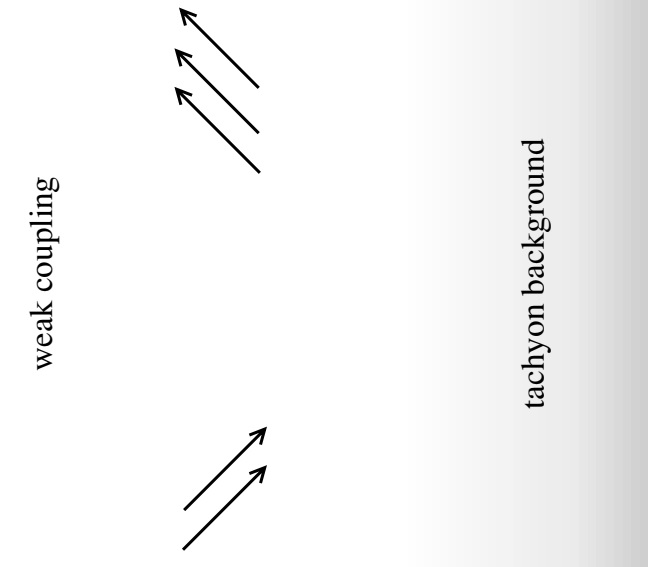
\includegraphics[width=0.8\textwidth]{figure/Fig9.12.jpg}\\
		\caption{Spacetime with dilaton and tachyon in the background. The further to the right, the stronger the interaction, but it is cut off by an effective potential from the tachyon background.}\label{Fig9.12}
	\end{center}
\end{figure}
\vspace*{-0.7cm}

When $D>2$, although it has been argued that the tachyon background acts like a potential barrier, its physical effect is not very clear. 
However, there is another reason to focus on $D \leq 2$: these theories are actually solvable.
Let's first observe that when we quantize the string, gauge symmetry will take away two families of oscillators. 
This leaves nothing when $D \leq 2$—only the center of mass motion, a scalar.\footnote{For some special momenta, extra physical states are found. They can be interpreted as unbroken symmetries of string field theory and may play a role in the solvability of the theory.} However, directly solving this string theory is quite difficult. First, the world-sheet path integral with the action \eqref{9.9.5} must be calculated. 
Due to the exponential tachyon field, this is no longer a free theory. It is called Liouville field theory.
It is classically integrable, and after some effort, some quantum amplitudes can be determined. 
However, to solve string theory, we need to integrate this result over every genus in the Riemann surface moduli space; we have seen that this is a compact space. 
Quite remarkably, amplitudes up to all orders have been determined through a quite different method. To describe this method, we must first introduce another concept.

\subsection*{Non-critical strings}

Consider a statistical mechanics system defined by summing over two-dimensional surfaces in $d$-dimensional Euclidean space. We also assume that the surfaces have some internal degrees of freedom that can be interpreted as a measure of length.
The natural fields to describe this system are the embedding $X^{\mu}(\sigma)$ and the metric $g_{a b}(\sigma)$. However, there is no reason to throw the length out of this problem—that is, the theory is not necessarily Weyl invariant. 
Thus it is called a non-critical string. The lowest dimensional action for this system is the Polyakov action with an extra world-sheet constant term, such as would be prohibited by Weyl invariance in critical strings:
\begin{equation}
	S=\frac{1}{4 \pi \alpha^{\prime}} \int_{M} \dif^{2} \sigma \: g^{1/2} 
	\Bigl(g^{ab} \partial_{a} X^{\mu} \partial_{b} X_{\mu}+\mu\Bigr) \:.
	\label{9.9.6}
\end{equation}

Without Weyl invariance, we can partially determine the metric with diff-invariance, but one degree of freedom will remain:
\begin{equation}
	g_{ab}(\sigma)=\exp (2 \phi(\sigma)) \hat{g}_{ab}(\sigma) \:, \label{9.9.7}
\end{equation}
where $\hat{g}_{ab}$ is a gauge choice, and the metric scale $\phi$ still needs to be integrated in the path integral. A gauge-fixed Faddeev-Popov determinant is the same as \eqref{3.4.19}, 
and the contribution of Weyl fixing to the latter is trivial.
Substituting the metric \eqref{9.9.7}, the curvature is:
\begin{equation}
	g^{1/2} R = \hat{g}^{1/2}\Bigl(\hat{R}-2 \hat{\nabla}^{2} \phi\Bigr) \:, \label{9.9.8}
\end{equation}
\begin{tcolorbox}[breakable]
	\begin{remark}
		Locally write $\hat g_{ab}=\me^{2\hat\omega}\delta_{ab}$. In two dimensions $R[\me^{2\omega}\delta]=-2\me^{-2\omega}\partial^2\omega$ with $\partial^2$ the flat Laplacian, and $\hat\nabla^2=\me^{-2\hat\omega}\partial^2$ on scalars. Then
		\begin{equation*}
			g^{1/2}R\eqs{1}\me^{2\phi+2\hat\omega}\cdot\bigl(-2\me^{-2\phi-2\hat\omega}\partial^2(\phi+\hat\omega)\bigr)=-2\partial^2\hat\omega-2\partial^2\phi\eqs{2}\hat g^{1/2}\bigl(\hat R-2\hat\nabla^2\phi\bigr).
		\end{equation*}
		At (1) $g=\me^{2(\phi+\hat\omega)}\delta$. At (2) $-2\partial^2\hat\omega=\hat g^{1/2}\hat R$ and $\partial^2\phi=\me^{2\hat\omega}\hat\nabla^2\phi=\hat g^{1/2}\hat\nabla^2\phi$. Both sides are covariant, so the local result holds globally. In particular $\int g^{1/2}R$ is independent of $\phi$, which is Gauss--Bonnet.
	\end{remark}
\end{tcolorbox}
throwing away field-independent terms, this action plus the Faddeev-Popov determinant becomes:
\begin{equation}
	S=\frac{1}{4 \pi \alpha^{\prime}} \int_{M} \dif^{2} \sigma \: \hat{g}^{1/2} \biggl[\hat{g}^{ab} \partial_{a} X^{\mu} \partial_{b} X_{\mu}+\mu \exp 2 \phi + \frac{13 \alpha^{\prime}}{3}\Bigl(\hat{g}^{ab} \partial_{a} \phi \partial_{b} \phi+\hat{R} \phi\Bigr)\biggr]\:.
	\label{9.9.9}
\end{equation}
Note that the Faddeev-Popov determinant provides a kinetic energy term for $\phi$.
\begin{tcolorbox}[breakable]
	\begin{remark}
		Conventions (Section \ref{sec:3.4}). For a CFT of central charge $c$, $\delta_{\mathrm W}\ln Z=-\frac{1}{2\pi}\int\dif^2\sigma\,g^{1/2}\delta\omega\,T^a{}_a$ with $T^a{}_a=-\frac{c}{12}R$. As in the text, the $X^\mu$ path integral is still defined with the full metric $g$. Only the ghost determinant is rewritten in terms of $\hat g$, so the relevant central charge is $c^{\mathrm g}=-26$.

		\emph{Integrated anomaly.} Along the path $g_s=\me^{2s\phi}\hat g$, $0\le s\le1$, we have $\delta\omega=\phi\,\dif s$ and $g_s^{1/2}R_s=\hat g^{1/2}(\hat R-2s\hat\nabla^2\phi)$ by \eqref{9.9.8}. Then
		\begin{align*}
			\ln\frac{Z[\me^{2\phi}\hat g]}{Z[\hat g]}&\eqs{1}\frac{c}{24\pi}\int_0^1\dif s\int\dif^2\sigma\,\hat g^{1/2}\phi\bigl(\hat R-2s\hat\nabla^2\phi\bigr)
			=\frac{c}{24\pi}\int\dif^2\sigma\,\hat g^{1/2}\bigl(\phi\hat R-\phi\hat\nabla^2\phi\bigr)\\
			&\eqs{2}\frac{c}{24\pi}\int\dif^2\sigma\,\hat g^{1/2}\bigl(\hat g^{ab}\partial_a\phi\partial_b\phi+\hat R\phi\bigr) .
		\end{align*}
		At (1) $\delta_{\mathrm W}\ln Z=\frac{c}{24\pi}\int g^{1/2}R\,\delta\omega$. At (2) the $\phi\hat\nabla^2\phi$ term was integrated by parts.

		\emph{Coefficient in \eqref{9.9.9}.} For the ghosts $c=-26$, so the determinant contributes $\me^{-S_\phi}$ with
		\begin{equation*}
			S_\phi=\frac{26}{24\pi}\int\hat g^{1/2}\bigl(\hat g^{ab}\partial_a\phi\partial_b\phi+\hat R\phi\bigr)=\frac{1}{4\pi\alpha'}\cdot\frac{13\alpha'}{3}\int\hat g^{1/2}\bigl(\hat g^{ab}\partial_a\phi\partial_b\phi+\hat R\phi\bigr),
		\end{equation*}
		since $\frac{26}{24\pi}=\frac{13}{12\pi}=\frac{1}{4\pi\alpha'}\cdot\frac{13\alpha'}{3}$. The cosmological term is $\mu g^{1/2}=\mu\,\me^{2\phi}\hat g^{1/2}$, and $g^{1/2}g^{ab}$ is Weyl invariant, so the $X$ kinetic term keeps its form. This reproduces \eqref{9.9.9}.

		If the $X^\mu$ measure were also converted to $\hat g$, their $c=d$ would change $26\to26-d$. Making $\phi$ itself a free field with measure defined by $\hat g$ adds its own $c=1$. These are the ``somewhat different coefficients'' mentioned in the text. Once they are included, $\phi$ becomes the linear dilaton direction $X^1$ with $D=d+1$: $V_1^2=(26-D)/6\alpha'$ matches $(25-d)/6\alpha'$ (the Distler--Kawai--David result, quoted here, not derived).
	\end{remark}
\end{tcolorbox} Compared with the dilaton-tachyon action \eqref{9.9.5}, we see a remarkable similarity. 
If we set $d=D-1$ and interpret the new field $\phi$ as $x^{1}$, and rename $g_{a b} \to \hat{g}_{a b}$ in action \eqref{9.9.5}, then the same terms appear. 
Some coefficients will be somewhat different—there is no rescaling of $\phi$ that makes them all consistent—but in fact, we claim they are the same field theory.
The key is that the critical string path integral \eqref{9.9.5} is defined using $\hat{g}_{ab}$ as the metric, while non-critical strings \eqref{9.9.9} use $\exp (2 \phi) \hat{g}_{a b}$. 
A careful treatment of the Weyl transformation of the measure can convert one to the other.
To understand this, note that only the total metric \eqref{9.9.7} appears in the definition of critical strings, so in the transformation:
\begin{subequations} \label{9.9.10}
	\begin{align}
		\hat{g}_{a b}(\sigma)  &\rightarrow \exp (2 \omega(\sigma)) \hat{g}_{a b}(\sigma) \:,  \label{9.9.10a}\\
		\phi(\sigma) &\rightarrow \phi(\sigma)-\omega(\sigma) \:, \label{9.9.10b}
	\end{align}
\end{subequations}
all quantities are invariant.
Thus non-critical strings gain Weyl invariance, which is sufficient to fix various coefficients other than the free parameter $\mu$.

A Weyl-invariant theory and a non-Weyl-invariant theory can be equivalent, which seems strange. The key is that in field theory, if we simultaneously increase the fields used only to fix the gauge, we can always add extra ``fake'' gauge symmetry. 
After all, a gauge symmetry is just a redundant description, and we can always adopt a more redundant description. For the symmetry \eqref{9.9.10}, we can obviously just cancel the Weyl symmetry of field $\phi$. 
But for general string backgrounds (for example, flat space, where the embedding coordinates are Weyl invariant), this is impossible, and Weyl invariance is ``real.''
In any case, we have now reached a very subtle situation where we can approximate non-critical strings by summing over triangulated surfaces, where the number of edges between two points becomes a measure of length. 
These triangulated surfaces are similar to large Feynman diagrams, and in fact we can find a quantum system—matrix model, which is a diagrammatic expansion. 
The fields of the matrix model are $N \times N$ matrices. Taking $N \rightarrow \infty$ and adjusting other couplings, (at least for $D \leq 2$) there exists a critical point dominated by smooth large surfaces, 
so we recover non-critical strings.
Furthermore, by diagonalizing the matrix (at least for $D \leq 2$), the matrix model is solvable. 
At the end, we obtain a quite simple system (non-interacting fermions moving in the eigenvalue space), and reversing the above steps allows for the calculation of string amplitudes to any order.

We leave the details to the references. In any case, when $D>2$ or in supersymmetric theories, they have not yet been found to be useful. 
However, at least we mention an important lesson learned from these models. The $(2g)!$ behavior in perturbation theory was originally seen in explicit matrix models, and from this, it was argued that it holds for all string theories.
In matrix models, the corresponding $\exp [O(-1 / g_{\mathrm{c}})]$ effects include tunneling of fermions in the eigenvalue space. 
Whether this is related to $\exp [O(-1 / g_{\mathrm{c}})]$ effects in higher dimensional string theories is still unclear.